% !TeX spellcheck = es_ES
\documentclass[twoside,openright,spanish,12pt,Grado]{licthesis_modIV}%,mydraft

% librerias de circuitos
%\usepackage{pstricks,pstricks-pdf,pst-node,pst-circ,pst-plot,pst-3dplot,pst-all}
\usepackage[siunitx]{circuitikz}
\usepackage[utf8]{inputenc}
\usepackage[siunitx]{circuitikz}
\usepackage[utf8]{inputenc}
\pagestyle{empty}
\usepackage{tikz}
\usepackage{xcolor}
\usepackage{listings}


\definecolor{mGreen}{rgb}{0.1,0.6,0}
\definecolor{mGray}{rgb}{0.5,0.5,0.5}
\definecolor{mPurple}{rgb}{0.80,0,0.82}
\definecolor{backgroundColour}{rgb}{0.95,0.95,0.92}

\lstdefinestyle{CStyle}{
	backgroundcolor=\color{backgroundColour},   
	commentstyle=\color{mGreen},
	keywordstyle=\color{magenta},
	numberstyle=\tiny\color{mGray},
	stringstyle=\color{mPurple},
	basicstyle=\footnotesize,
	breakatwhitespace=false,         
	breaklines=true,                 
	captionpos=b,                    
	keepspaces=true,                 
	numbers=left,                    
	numbersep=5pt,                  
	showspaces=false,                
	showstringspaces=false,
	showtabs=false,                  
	tabsize=2,
	language=C
}


\usepackage{etoolbox}
\usepackage{titlesec}
\usepackage{soul}
\usepackage{url}
\usepackage[spanish,es-tabla]{babel}   % para escribir en castellano
\usepackage[utf8]{inputenc}   % para tipo de caracteres de entrada
\usepackage{graphicx}         % para insertar graficos *.eps
\usepackage{listings}
\usepackage[cmex10]{amsmath}  % simbolos matem\'{a}ticos extendidos
\usepackage{amssymb}          % simbolos matem\'{a}ticos extendidos
\usepackage{latexsym}         % S\'{\i}mbolos
\usepackage{makeidx}          % para generar el indice
%\usepackage{subfigure}
\usepackage{subcaption}
\usepackage{cases}
\usepackage[normalem]{ulem}
%\usepackage{natbib}
%\usepackage{jurabib}
%\usepackage{grffile}
\usepackage[final]{pdfpages}
\usepackage{enumerate}
\usepackage{array} %centrar verticalmente en tablas
\usepackage{float}
%\usepackage{CJKutf8}
%\usepackage[spanish,numbers]{flexbib}
\usepackage[numbers,sort]{natbib}
\usepackage{notoccite} % Evitar que las citas en los caption inicien el contador (aparecen en la lista de figuras)
\usepackage{layouts}
\usepackage{newverbs}
\usepackage{xpatch}
\usepackage{algorithm} %ctan.org\pkg\algorithms
%\usepackage{algorithmic}
\usepackage{algpseudocode}
\makeatletter
	\xpatchcmd{\algorithmic}{\itemsep\z@}{\itemsep=-4pt}{}{}
\makeatother
\floatname{algorithm}{Algoritmo} %Cambiar el titluo del float a español
\renewcommand{\listalgorithmname}{Índice de algoritmos}
\makeatletter %Para numerar los algoritmos como (num de capitulo).(num de algoritmo)
	\renewcommand\thealgorithm{\thechapter.\arabic{algorithm}} 
	\@addtoreset{algorithm}{chapter} 
\makeatother
%\floatname{algorithm}{Algoritmo}
\renewcommand{\listalgorithmname}{Lista de algoritmos}
\renewcommand{\algorithmicrequire}{\textbf{Entrada:}}
\renewcommand{\algorithmicensure}{\textbf{Salida:}}
\renewcommand{\algorithmicend}{\textbf{fin}}
\renewcommand{\algorithmicif}{\textbf{si}}
\renewcommand{\algorithmicthen}{\textbf{entonces}}
\renewcommand{\algorithmicelse}{\textbf{si no}}
%\renewcommand{\algorithmicelsif}{\algorithmicelse,\ \algorithmicif}
%\renewcommand{\algorithmicendif}{\algorithmicend\ \algorithmicif}
\renewcommand{\algorithmicfor}{\textbf{para}}
\renewcommand{\algorithmicforall}{\textbf{para todo}}
\renewcommand{\algorithmicdo}{\textbf{hacer}}
%\renewcommand{\algorithmicendfor}{\algorithmicend\ \algorithmicfor}
\renewcommand{\algorithmicwhile}{\textbf{mientras}}
%\renewcommand{\algorithmicendwhile}{\algorithmicend\ \algorithmicwhile}
\renewcommand{\algorithmicloop}{\textbf{repetir}}
%\renewcommand{\algorithmicendloop}{\algorithmicend\ \algorithmicloop}
\renewcommand{\algorithmicrepeat}{\textbf{repetir}}
\renewcommand{\algorithmicuntil}{\textbf{hasta que}}
%\renewcommand{\algorithmicprint}{\textbf{imprimir}} 
\renewcommand{\algorithmicreturn}{\textbf{devolver}} 
%\renewcommand{\algorithmictrue}{\textbf{cierto }} 
%\renewcommand{\algorithmicfalse}{\textbf{falso }} 
 %Traducción de los algoritmos
%% begin vertical rule patch for algorithmicx (http://tex.stackexchange.com/questions/144840/vertical-loop-block-lines-in-algorithmicx-with-noend-option)
\makeatletter
% start with some helper code
% This is the vertical rule that is inserted
    \newcommand*{\algrule}[1][\algorithmicindent]{\makebox[#1][l]{\hspace*{.5em}\thealgruleextra\vrule height \thealgruleheight depth \thealgruledepth}}%
% its height and depth need to be adjustable
\newcommand*{\thealgruleextra}{}
\newcommand*{\thealgruleheight}{.75\baselineskip}
\newcommand*{\thealgruledepth}{.25\baselineskip}

\newcount\ALG@printindent@tempcnta
\def\ALG@printindent{%
    \ifnum \theALG@nested>0% is there anything to print
        \ifx\ALG@text\ALG@x@notext% is this an end group without any text?
            % do nothing
        \else
            \unskip
            \addvspace{-1pt}% FUDGE to make the rules line up
            % draw a rule for each indent level
            \ALG@printindent@tempcnta=1
            \loop
                \algrule[\csname ALG@ind@\the\ALG@printindent@tempcnta\endcsname]%
                \advance \ALG@printindent@tempcnta 1
            \ifnum \ALG@printindent@tempcnta<\numexpr\theALG@nested+1\relax% can't do <=, so add one to RHS and use < instead
            \repeat
        \fi
    \fi
    }%
\usepackage{etoolbox}
% the following line injects our new indent handling code in place of the default spacing
\patchcmd{\ALG@doentity}{\noindent\hskip\ALG@tlm}{\ALG@printindent}{}{\errmessage{failed to patch}}
\makeatother

% the required height and depth are set by measuring the content to be shown
% this means that the content is processed twice
\newbox\statebox
\newcommand{\myState}[1]{%
    \setbox\statebox=\vbox{#1}%
    \edef\thealgruleheight{\dimexpr \the\ht\statebox+1pt\relax}%
    \edef\thealgruledepth{\dimexpr \the\dp\statebox+1pt\relax}%
    \ifdim\thealgruleheight<.75\baselineskip
        \def\thealgruleheight{\dimexpr .75\baselineskip+1pt\relax}%
    \fi
    \ifdim\thealgruledepth<.25\baselineskip
        \def\thealgruledepth{\dimexpr .25\baselineskip+1pt\relax}%
    \fi
    %\showboxdepth=100
    %\showboxbreadth=100
    %\showbox\statebox
    \State #1%
    %\State \usebox\statebox
    %\State \unvbox\statebox
    %reset in case the next command is not wrapped in \myState
    \def\thealgruleheight{\dimexpr .75\baselineskip+1pt\relax}%
    \def\thealgruledepth{\dimexpr .25\baselineskip+1pt\relax}%
}
% end vertical rule patch for algorithmicx %Agrega lineas verticales el en el algoritmo

% Excel2LaTeX.xla
\usepackage{multirow}
\usepackage{booktabs}
\usepackage{bigstrut}
\usepackage{mathtools}
\usepackage{pdflscape}
\usepackage{bibentry}
\nobibliography*
\usepackage{longtable}
\usepackage{afterpage}
\usepackage{colortbl}
\usepackage{multicol}
\usepackage{amsmath}
%% % % % COLOR Y CAJAS PARA ECUACIONES % % % % %
%	\usepackage{color}
%	\definecolor{myblue}{rgb}{.9, .9, .9}
%	\usepackage{empheq}
%	
%	\newlength\mytemplen
%	\newsavebox\mytempbox
%	
%	\makeatletter
%	\newcommand\mybluebox{%
%	    \@ifnextchar[%]
%	       {\@mybluebox}%
%	       {\@mybluebox[0pt]}}
%	
%	\def\@mybluebox[#1]{%
%	    \@ifnextchar[%]
%	       {\@@mybluebox[#1]}%
%	       {\@@mybluebox[#1][0pt]}}
%	
%	\def\@@mybluebox[#1][#2]#3{
%	    \sbox\mytempbox{#3}%
%	    \mytemplen\ht\mytempbox
%	    \advance\mytemplen #1\relax
%	    \ht\mytempbox\mytemplen
%	    \mytemplen\dp\mytempbox
%	    \advance\mytemplen #2\relax
%	    \dp\mytempbox\mytemplen
%	    \colorbox{myblue}{\hspace{5pt}\usebox{\mytempbox}\hspace{5pt}}}
%	
%	\makeatother
%% % % % % % % % % % % % % % % % % % % % % % % % % % % % %




\let\includegraphicsWithoutCF=\includegraphics
\renewcommand{\includegraphics}[2][]{\includegraphicsWithoutCF[#1]{\currentfolder figuras/#2}}
\newcommand{\currentfolder}{}
\newcommand{\chapterlabel}[1]{\label{#1}\renewcommand{\currentfolder}{#1/}}

\let\inputCF=\input
\newcommand{\inputfig}{}
\renewcommand{\inputfig}[1]{\inputCF{\currentfolder figuras/#1.pdf_tex}}
\renewcommand{\input}[1]{\inputCF{\currentfolder #1}}

%\let\subrefWithoutProtect\subref
%\renewcommand{\subref}[1]{\protect\subrefWithoutProtect{#1}}

\newcommand{\sectionname}{Secci\'{o}n}
\newcommand{\equationname}{Ecuaci\'{o}n}
%\tablespagefalse

\usepackage{colortbl}
\newcommand{\cc[1]}{\cellcolor[rgb]{0.9,0.9,0.9}}

\RequirePackage[bookmarksnumbered,colorlinks,hyperindex,a4paper]{hyperref}  % crea hipervinculos en el indice
\hypersetup{linkcolor=blue,%
            citecolor=red,%
            pdfstartview=FitH,%
            pdftoolbar=true,%
            bookmarksopen=false,%
            bookmarksopenlevel=\maxdimen,
            urlcolor=red}  % color of external links
\def\pdfBorderAttrs{/Border [0 0 0] } % Ning\'{u}n borde a los links

%\setcounter{MaxMatrixCols}{30}
%\clubpenalty=9999
%\widowpenalty=9999

\newtheorem{theorem}{Theorem}
\newtheorem{acknowledgement}[theorem]{Acknowledgement}
%\newtheorem{algorithm}[theorem]{Algorithm}
\newtheorem{axiom}[theorem]{Axiom}
\newtheorem{case}[theorem]{Case}
\newtheorem{claim}[theorem]{Claim}
\newtheorem{conclusion}[theorem]{Conclusion}
\newtheorem{condition}[theorem]{Condition}
\newtheorem{conjecture}[theorem]{Conjecture}
\newtheorem{corollary}[theorem]{Corollary}
\newtheorem{criterion}[theorem]{Criterion}
\newtheorem{definition}[theorem]{Definition}
\newtheorem{example}[theorem]{Example}
\newtheorem{exercise}[theorem]{Exercise}
\newtheorem{lemma}[theorem]{Lemma}
\newtheorem{notation}[theorem]{Notation}
\newtheorem{problem}[theorem]{Problem}
\newtheorem{proposition}[theorem]{Proposition}
\newtheorem{remark}[theorem]{Remark}
\newtheorem{solution}[theorem]{Solution}
\newtheorem{summary}[theorem]{Summary}
\newenvironment{proof}[1][Proof]{\textbf{#1.} }{\ \rule{0.5em}{0.5em}}


\def\sen{\mathop{\mbox{\normalfont sen}}\nolimits}
%\renewcommand{\arraystretch}{1.2}
\setlength{\minrowclearance}{1mm}
%\renewcommand{\arraystretch}{1.8}
\setlength{\intextsep}{10mm}
%\renewcommand{\tabcolsep}{2mm}
\newcommand{\on}[1]{\operatorname{#1}}           % Unidades
\newcommand{\mx}[2]{\left[\begin{array}{#1}#2\end{array}\right]}           % Vector o matriz
\setlength\arraycolsep{0.15em}
\newcommand{\dif}[1]{\mathop{#1}\limits^\bullet} % Diferencial de una variable
\newcommand{\m}[1]{\mathbf{#1}}         % Variables matriciales

%\newcommand{\eq}[1]{Ec.~(\ref{eq:#1})}  % Referenciar una ecuacion
\newcommand{\eq}[1]{\mbox{\hyperref[#1]{Ec.~(\ref{eq:#1})}}}
%\newcommand{\eqs}[1]{(\ref{eq:#1})}     % Referenciar ecuaciones
\newcommand{\eqs}[1]{\mbox{\hyperref[#1]{(\ref{eq:#1})}}}
%\newcommand{\fig}[1]{Figura~\ref{fig:#1}}  % Referenciar una figura
\newcommand{\fig}[1]{\mbox{\hyperref[fig:#1]{Figura~\ref{fig:#1}}}}
\newcommand{\figs}[1]{\ref{fig:#1}}        % Referenciar figuras
%\newcommand{\tab}[1]{Tabla~(\ref{tab:#1})} % Referenciar una tabla
\newcommand{\tab}[1]{\mbox{\hyperref[tab:#1]{Tabla~(\ref{tab:#1})}}} % Referenciar una tabla

\newcommand{\ch}[1]{\mbox{\hyperref[#1]{Cap\'\i tulo~\ref{#1}}}}       % Referenciar capitulos
\newcommand{\apx}[1]{\mbox{\hyperref[#1]{Ap\'endice~\ref{#1}}}}        % Referenciar figuras
\newcommand{\secc}[1]{\mbox{\hyperref[#1]{Secci\'on~\ref{#1}}}}


\newcommand{\C}{\operatorname{{}^{\circ}{\rm C}}} % Grados (temperatura)

\def\substring#1#2#3{\expandafter\subm\romannumeral#3000x.{}#1\relax\relax{#2}}
\def\subm#1#2.#3#4\relax#5\relax{\csname sub#1\endcsname#2.#4\relax#5#3\relax}
\def\subx#1.#2\relax#3\relax#4{\expandafter\submb\romannumeral#4000x.{}{}#3\relax}
\def\submb#1#2.#3{\csname sub#1b\endcsname#2.}
\def\subxb#1.#2\relax{#2}


\newcommand{\se}[1]{{
    \mathrm{\uppercase{\substring{#1}{1}{1}}}
    _\mathrm{\uppercase{\substring{#1}{2}{2}}}
    \mathrm{\uppercase{\substring{#1}{3}{3}}}
    _\mathrm{\uppercase{\substring{#1}{4}{4}}}
    \mathrm{\uppercase{\substring{#1}{5}{5}}}
    _\mathrm{\uppercase{\substring{#1}{6}{6}}}}}

%********************Separado en silabas correcto******************************************************
\hyphenation{na-tu-ral trans-fe-ren-cia res-pues-tas consta mo-du-la-cion cons-tru-ir co-rrien-te}
\hyphenation{su-mi-nis-trar e-fec-tua-das ins-pi-ra-do sa-cri-fi-cio erro-res esta-ble-ci-mien-to}
\hyphenation{aproxi-ma-das pre-sin-cro-nis-mo megadiscap}


%*************************Comienzo del documento Tesis*************************************************


\makeindex

%\includeonly{
%%introduccion/introduccion,
%%sintesis/sintesis,
%control/control,
%%experimentales/experimentales,
%%conclusiones/conclusiones,
%%%
%%CE/CE,
%%thermal/thermal,
%%dinamica/dinamica,
%%digital/digital,
%%almacenamiento/almacenamiento,
%%megadiscap/megadiscap,
%}

\DeclarePairedDelimiter{\abs}{\lvert}{\rvert}%

% % % % % % % % % % 
% % NOMENCLATURA % %

	\newcommand{\rip}{{\Delta i_T}} 				%Ripple total
	\newcommand{\itot}{i_T} 					%Corriente total
	\newcommand{\itotmean}{\bar{i_T}}			%Corriente media total
	\newcommand{\iphase}[1]{i_{#1}}				%Corriente de fase
	\newcommand{\ierr}[1]{i_{e_{#1}}}			%Error de corriente
	\newcommand{\iref}{i_{\mathit{Ref}}}		%Ref de corriente.
	\newcommand{\pwm}[1]{\text{PWM}_{#1}}		%PWMj
	\newcommand{\sync}[1]{\mathit{Sync_{#1}}}	%SINCj
	\newcommand{\switch}[1]{T_{#1}}				%Switch de fase
	\newcommand{\Lj}[1]{L_{#1}}					%Inductor de fase
 	\newcommand{\fswitch}{f_{sw}}				%Frec. de conmutacion.
 	\newcommand{\tswitch}{{T_{sw}}}				%Frec. de conmutacion.
 	\newcommand{\tsync}{T_{\mathit{Sync}}}		%Periodo de sinc.
	\newcommand{\rms}{\mathit{RMS}}				%RMS
	\newcommand{\spo}{{s_p}}					%Pendiente positiva
	\newcommand{\sne}{{s_n}}					%Pendiente negativa
	\newcommand{\tclk}{{T_{CLK}}}               %Periodo de clock
	
 	%Caracterizacion
	
	\newcommand{\ripcart}{{r_{\!\!_{T}}}} 		%Ripple total 
	\newcommand{\ripcarp}[1]{r_{#1}} 			%Ripple fase 
	\newcommand{\peakt}[2]{{P_{\!#1}^{_#2}}} 	%Pico ripple tot 
	\newcommand{\tgenp}{t_x^{+}} 				%Tiempo generico tx
	\newcommand{\tgenn}{t_x^{-}} 				%Tiempo generico tx
	\newcommand{\esr}{\mathit{ESR}}             %ESR del capacitor
	
% % % % % % % % % % 
% % % % % % % % % %

% AGREGADO PARA CREAR SUBSUBSUB-SECTIONS
\titleclass{\subsubsubsection}{straight}[\subsection]

\newcounter{subsubsubsection}[subsubsection]
\renewcommand\thesubsubsubsection{\thesubsubsection.\arabic{subsubsubsection}}
\renewcommand\theparagraph{\thesubsubsubsection.\arabic{paragraph}} % optional; useful if paragraphs are to be numbered

\titleformat{\subsubsubsection}
{\normalfont\normalsize\bfseries}{\thesubsubsubsection}{1em}{}
\titlespacing*{\subsubsubsection}
{0pt}{3.25ex plus 1ex minus .2ex}{1.5ex plus .2ex}

\makeatletter
\renewcommand\paragraph{\@startsection{paragraph}{5}{\z@}%
	{3.25ex \@plus1ex \@minus.2ex}%
	{-1em}%
	{\normalfont\normalsize\bfseries}}
\renewcommand\subparagraph{\@startsection{subparagraph}{6}{\parindent}%
	{3.25ex \@plus1ex \@minus .2ex}%
	{-1em}%
	{\normalfont\normalsize\bfseries}}
\def\toclevel@subsubsubsection{4}
\def\toclevel@paragraph{5}
\def\toclevel@paragraph{6}
\def\l@subsubsubsection{\@dottedtocline{4}{12em}{4em}}
\def\l@paragraph{\@dottedtocline{5}{10em}{5em}}
\def\l@subparagraph{\@dottedtocline{6}{14em}{6em}}
\makeatother
%


%Para cambiar símbolos en los enumerados
%\renewcommand{\labelitemi}{$-$}
\renewcommand{\labelitemii}{$-$}
\renewcommand{\labelitemiii}{$cDot$}
%





%Para poder tener más subsecciones
\setcounter{secnumdepth}{6} 
\setcounter{tocdepth}{6}

\begin{document}
\raggedbottom

%% Inserta p\'{a}gina en blanco para imprimir dos p\'{a}ginas por hoja
%\NoBgThispage
%\thispagestyle{empty}
%\setcounter{page}{0}
%\begin{flushright}
%\textcolor[rgb]{1.00,1.00,1.00}{P\'{a}gina intencionalmente vac\'{\i}a.}
%\end{flushright}
%\newpage

\title{Modelo de levitador magnético experimental para práctica docente}
\shorttitle{}
\englishtitle{}

\author{Juan Manuel Guariste \\ Ignacio Islas \\ Javier Mosconi}
\authoreng{}

\departamento{Departamento de Electrónica y Computación}

\director{Ing. Walter Kloster}
\codirector{Ing. Gustavo Uicich}

\thesisdate{día X de Mayo del año 2022}
\thesisdateeng{}

\dedication{\textit{	COMPLETAR la "DEDICATION" que se encuentra junto con "title" en el Master.tex	.}}

\affiliation{El presente trabajo fue realizado en el Laboratorio de Instrumentación y Control del Departamento de Electrónica y Computación, ICyTE, Facultad de Ingeniería, Universidad Nacional de Mar del Plata.}
\englishaffiliation{This thesis work has been carried out in the Instrumentation and Control Laboratory, ICyTE, School of Engineering, National University of Mar del Plata.}
%\chapter*{dedication}
%\pagenumbering{Roman} % para comenzar la numeracion de paginas en numeros romanos
\begin{flushright}
\textit{
A mi familia y amigos, por ser mi sostén desde el primer momento.}
\end{flushright}

\beforeabstract

\chapter*{\textit{Agradecimientos}} % si no queremos que añada la palabra "Capitulo"
%\addcontentsline{toc}{chapter}{Agradecimientos} % si queremos que aparezca en el índice
\markboth{AGRADECIMIENTOS}{AGRADECIMIENTOS} % encabezado 

\begin{flushright}
%Pablo Daniel Antoszczuk \\ Mar del Plata, 11 de diciembre de 2014.
%Marco Carnaghi\\ Mar del Plata, 22 de marzo de 2019.

% MARCO: A Pablo y Paula, por acompañarme, enseñarme y estar a mi lado durante todo el proyecto. Además, la paciencia y dedicación que aportaron a todo el trabajo realizado. A Rogelio, por su aporte incondicional durante el proceso. A Marcos, por abrirme las puertas a trabajar en el laboratorio.


 
\end{flushright}

\afterabstract
\afterpreface

%------------------------------- CAP\'{I}TULOS -------------------------------

\chapter{Controlador} \chapterlabel{Controlador} \label{cap:Controlador}

\section{Controlador}

A lo largo de este documento se ha explicado la investigación, desarrollo e implementación del sistema SAE para automatizar playas de estacionamiento. Se decidió trabajar de manera incremental. Por lo tanto, se desarrolló un prototipo inicial, el cual fue progresando a medida que se avanzaba en el proyecto, debido al agregado de nuevas funcionalidades y la mejora de las ya existentes, hasta obtener un prototipo final. Mientras en el inicial se hizo hincapié en el funcionamiento de algunas etapas de gran importancia y complejidad, como es el caso de la detección de patentes, el final se enfocó en la parte de hardware. 

En el primer capítulo, se desarrolló el sistema como un producto comercial, tal como fue pensado en conjunto con la empresa que apoya este proyecto. Luego, se explicó su funcionamiento, tanto para el caso del ingreso como para el del egreso. Además, junto con los directores del trabajo final, con el objetivo de limitar el tiempo de desarrollo del proyecto y su nivel de complejidad, se estableció el alcance del mismo. De esta manera, se dejaron fuera del mismo la entrega de los tickets al ingreso y la implementación de una pantalla para  la asignación de lote, entre otras. Esto se trata con más detalle en la sección siguiente.

Por otra parte, para determinar la ubicación más adecuada de los periféricos dentro de un posible estacionamiento, se llevó a cabo un relevamiento. El mismo se abocó a las características de los establecimientos que se encuentran en la zona céntrica de la ciudad de Mar del Plata. Una posible distribución de los mismos se observa en el esquema de la figura \ref{fig:img_croquis-est}.

Debido a que el reconocimiento de las patentes es un punto crítico de este proyecto, se ha llevado a cabo una investigación exhaustiva en torno al mismo. Mediante esta, se pudieron observar los diferentes tipos de sistemas ALPR existentes, su funcionamiento general y las ventajas y desventajas que presentan. Al tratarse de una etapa crucial, se tomó la decisión de analizar dos alternativas diferentes (OpenALPR y OpenCV 3 license plate recognition), para luego optar por una de ellas. Para ambos sistemas, se llevó a cabo un análisis en detalle de su funcionamiento, se experimentó con ellos y se realizó su ajuste en base a dicha experimentación. Para ello, fue necesaria la construcción de diversos conjuntos de imágenes. A partir de los resultados obtenidos, que fueron presentados en el Capítulo \ref{cap:alpr}, se decidió continuar trabajando con el software OpenALPR. Esto se debe, principalmente, a que con esta herramienta, al reconocer la matrícula, se obtiene un porcentaje de éxito mucho mayor y en menor tiempo que con la otra alternativa.  Además, en este capítulo se muestra el relevamiento hecho sobre las características de las matrículas argentinas, considerando el modelo antiguo y el del MERCOSUR.

El otro punto crucial del sistema es el desarrollo del hardware necesario. En el Capítulo \ref{cap:2do-nucleo} se presentó el diseño y construcción de la placa encargada de controlar los equipos que se ubicarían en las zonas de ingreso y egreso. Se realizó la muestra de los esquemas circuitales correspondientes a la fuente de alimentación del sistema y la parte lógica de la placa, junto con la justificación de las diversas decisiones que se tomaron durante el diseño. Además, se realizó una breve descripción de los elementos principales del PCB, que son el microcontrolador ATmega328P y el módulo de comunicación WiFi ESP-01, y de los periféricos que integran el sistema, que son el detector vehicular magnético y las barreras infrarrojas. Finalmente, se presentó el desarrollo e implementación del circuito impreso. Para la realización del mismo, fue necesario instruirse en el uso de Altium Designer y en el método de insolado para la fabricación de placas.

El funcionamiento del sistema se basa en tres códigos diferentes, que fueron desarrollados completamente, y se encuentran distribuidos en la UCC, la Placa I/O y el Módulo WiFi. Estos fueron diseñados con el objetivo de implementar la multiprogramación. Mediante esta técnica, la ejecución de tareas por parte del procesador se da a una velocidad que causa la impresión de que ocurren en paralelo. De esta manera, se le permitió al sistema SAE poder diferenciar entre las vías de ingreso y egreso, es decir, que puede realizar el proceso de entrada y de salida en "simultáneo". Por otra parte, se añadieron al sistema funcionalidades para responder ante algunos casos particulares, como por ejemplo, un vehículo que pretende retirarse sin efectuar el pago, uno que se retire de la vía de egreso hacia el interior del establecimiento, la obtención de la matrícula de un vehículo que desea egresar y que no se encuentra en la base de datos, entre otros.

Por último, deben destacarse las características distintivas que posee el prototipo obtenido. Las mismas se enumeran a continuación:

\begin{itemize}
	\item Los sistemas de automatización investigados, tanto los implementados en los establecimientos de nuestra ciudad como los ofrecidos por empresas radicadas en la ciudad de Buenos Aires, no poseen un sistema de reconocimiento de patentes ni un sistema de detección de tamaño estandarizado.
	\item No se encontraron fabricantes de este tipo de sistemas en Mar del Plata. El desarrollo de un sistema en la ciudad permite abastecer a los establecimientos locales y proporcionarles un servicio de mantenimiento (actualmente dependen de empresas radicadas en Bs.As.).
	\item El prototipo se encuentra desarrollado completamente mediante software libre. Esto evita el pago de licencias y, en el caso del software de reconocimiento de patentes, el pago de un servicio mensual.
\end{itemize}


\section{Trabajos futuros}

El objetivo de esta sección es dejar establecidas aquellas ideas o mejoras que pueden ser implementadas en un futuro en el sistema desarrollado. Esto se debe a que, al tratarse de un proyecto de finalización de una carrera universitaria, el mismo tiene un período acotado de duración, el cual hace que muchas de estas ideas deban mantenerse fuera del mismo.

\subsection{Mejoras}
\begin{itemize}
	\item Realizar el entrenamiento del motor de OCR específico para las matrículas argentinas
	\item Desarrollo de una base de datos más compleja, que ofrezca más opciones al operador del sistema
	\item Diseño de un sistema de reseteo remoto en caso de falla en el sistema
	\item Implementación de un sistema de respaldo en caso de corte de luz
	\item Diseño y construcción de una terminal que integre la UCC, en formato All in One, junto con el lector de código de barra y la impresora de tickets fiscales
\end{itemize}

\subsection{Nuevas funcionalidades}
\begin{itemize}
	\item Agregado de impresora de tickets internos al estacionamiento, con información de hora de ingreso, número de patente y tarifa, entre otras, con su correspondiente lector de código de barra
	\item Agregado de impresora de tickets fiscales
	\item Desarrollo de una interfaz de usuario que permita el ingreso de información por parte del operario en caso de que ocurra algún inconveniente
	\item Desarrollo de un algoritmo de asignación de ubicación dentro del establecimiento y verificación del correcto estacionamiento
	\item Agregado de pantalla para mostrar el resultado de la asignación de ubicación al cliente
	\item Automatización del cobro de la tarifa a los clientes
	\item Adaptación del sistema para su aplicación en cocheras de edificios comerciales y privados, control de ingreso y egreso a barrios cerrados, etc
	\item Detección de rostros al ingreso y egreso del establecimiento, de manera de incrementar la seguridad en cuanto al retiro de los vehículos
\end{itemize}



%\chapter{Estructura y funcionamiento del sistema completo} \chapterlabel{Estructura-sist} \label{cap:estructura sist}

\section{Introducción}
El propósito de este proyecto final es diseñar un prototipo a partir del cual la empresa pueda continuar con su desarrollo y obtener un producto. La versión comercial pensada a futuro en conjunto con la empresa puede observarse en el esquema de la figura \ref{fig:img_croquis-est}.

El objetivo de este capítulo es describir la estructura y funcionamiento del sistema completo a partir del cual se desarrollará el prototipo final.

\begin{itemize}
	\item \textcolor{mGreen}{Este no es el definitivo, ya que tiene los colores invertidos y líneas del AutoCAD.}
	\end{itemize}

\begin{figure}[H]
	\centering
	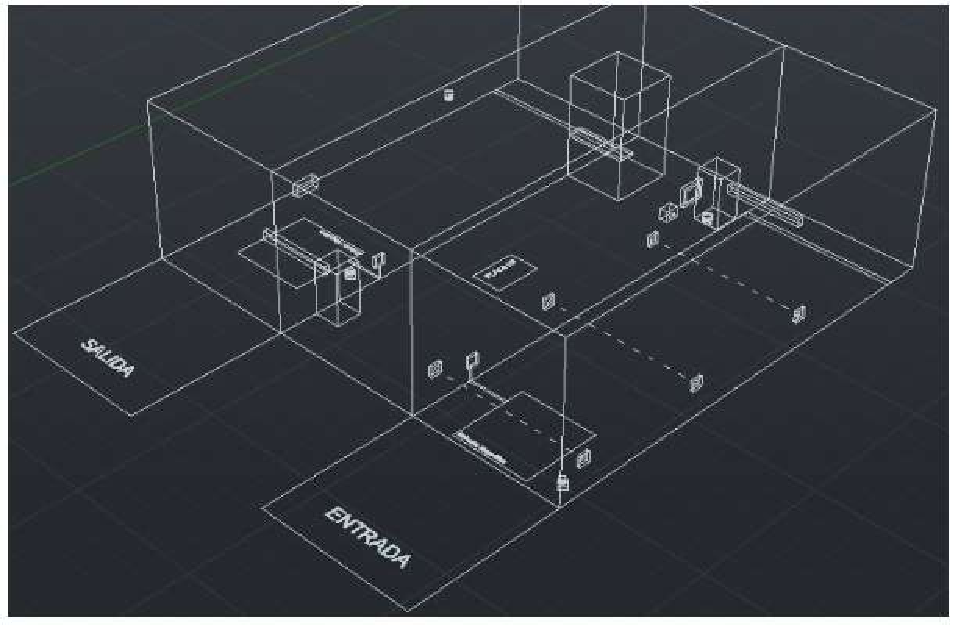
\includegraphics[width=\textwidth]{croquis.pdf}
	\caption{Producto pensado a futuro.}
	\label{fig:img_croquis-est}
\end{figure}

El sistema final fue planteado para un estacionamiento como el de la figura \ref{fig:img_croquis-est}, con vías de ingreso y egreso independientes. Sin embargo, el mismo es fácilmente adaptable a establecimientos que posean características diferentes. 

Basándonos en este modelo, el sistema posee tanto en el ingreso como en el egreso, una barrera vehicular, un detector magnético de presencia y dos cámaras IP.  Se utilizan dos cámaras debido a que las motocicletas no poseen patente delantera, mientras que los demás vehículos sí. Entonces, una apunta a la patente trasera y la otra a la delantera.

Además, en el ingreso se encuentra un mecanismo de detección de tipo (o tamaño) de vehículo implementado con tres barreras infrarrojas. Las mismas funcionan en conjunto con el detector magnético. En la vía de entrada se cuenta también con una pantalla que indica a los clientes el lote asignado y la información que el encargado del establecimiento desee mostrar, y una impresora de tickets internos al estacionamiento con código de barra.

Por último, dentro de la cabina del operador del sistema, se tiene la Unidad Central de Control (UCC), encargada de interactuar con todos los componentes del sistema y procesar los datos obtenidos por los mismos. Entre las tareas que desarrolla se encuentran obtener el número de la patente del vehículo que ingresa o egresa del estacionamiento y de gestionar la base de datos. Además, en la cabina también se cuenta con una impresora de tickets fiscales y un lector de código de barra.
 
Uno de los componentes fundamentales del sistema es la Placa I/O \hl{CAMBIAR NOMBRE DE LA PLACA} que concentra todos los periféricos de la zona de ingreso/egreso, menos las cámaras, y que se comunica con la UCC  mediante WI-FI.

\section{Funcionamiento}

En la figura \ref{fig:img_img-china} puede observarse el esquema de funcionamiento del sistema a un nivel general. El mismo se explica más detalladamente a lo largo de las dos siguientes secciones.

\begin{figure}[H]
	\centering
	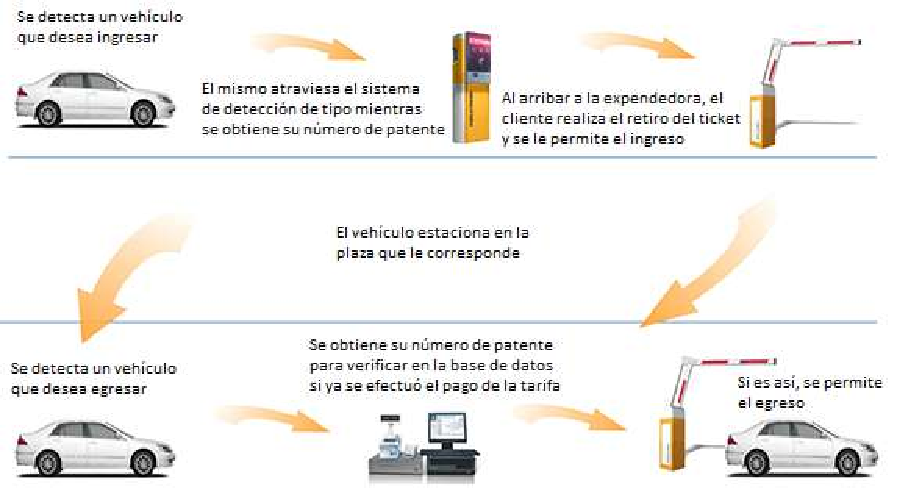
\includegraphics[scale=1]{img-china.pdf}
	\caption{Esquema general de funcionamiento del sistema.}
	\label{fig:img_img-china}
\end{figure}

A continuación, se describen los módulos de ingreso y egreso del sistema.

\subsection{Ingreso}

Como se observa en la figura \ref{fig:img_ingreso}, el proceso comienza con la detección de un vehículo que desea ingresar al estacionamiento. La misma se realiza mediante un detector magnético ubicado en el suelo, bajo el pavimento. Este posee una bobina (el lazo) cuya inductancia varía cuando un gran elemento metálico se acerca a ella. Esa variación hace que se modifique la frecuencia de oscilación del oscilador que posee el equipo. Esto produce la activación de un contacto seco que se utiliza para indicarle al sistema que un vehículo intenta ingresar al establecimiento.

\begin{figure}[H]
	\centering
	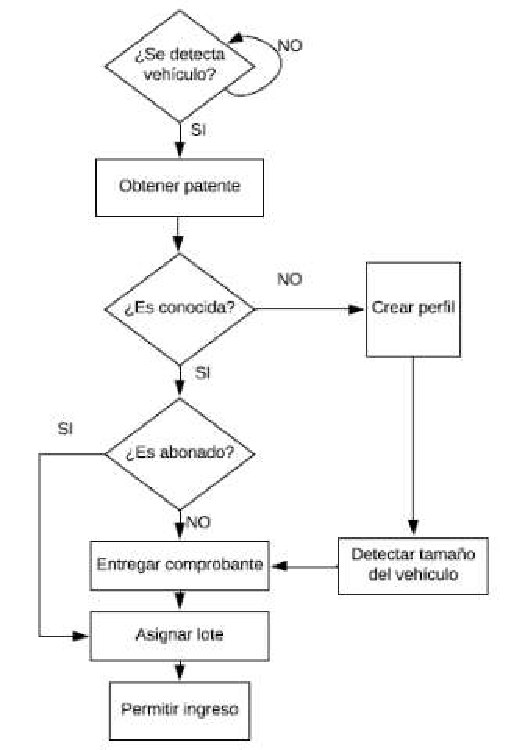
\includegraphics[scale=1]{func-ingreso.pdf}
	\caption{Funcionamiento del sistema en el ingreso.}
	\label{fig:img_ingreso}
\end{figure}

A continuación, se realiza la obtención de la patente mediante un juego de dos cámaras IP que se encuentran filmando continuamente. La misma es buscada en la base de datos y, en caso de no ser encontrada, se crea un perfil para el vehículo. Además, se determina el tamaño del mismo y se lo añade al perfil, con el objetivo de determinar la tarifa a cobrar (automóvil, camioneta o motocicleta). 

Luego, se procede a asignarle al conductor, mediante una pantalla, el lote en el que debe estacionarse, la hora de ingreso, la patente y la tarifa. Junto a la pantalla se encuentra una expendedora de tickets internos al estacionamiento, que poseen un código de barra y la misma información mostrada anteriormente. Los mismos se pueden retirar sin bajarse del vehículo. 

En caso de que el usuario sea abonado, no se le entrega el ticket debido a que el sistema reconoce la condición de abonado al detectar la patente.

Luego de que el usuario retire el ticket, se levanta la barrera y se permite el acceso. 


\subsection{Egreso}

Al igual que el de entrada, el sistema de egreso comienza con la detección de un vehículo que desee retirarse del establecimiento. El mismo puede observarse en la figura \ref{fig:img_egreso}. Una vez que esto sucede, se procede a obtener la patente del vehículo, con el fin de determinar si la tarifa ya fue pagada.

\begin{figure}[H]
	\centering
	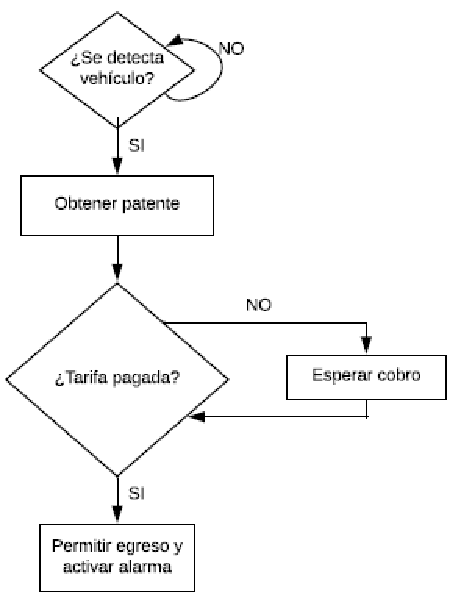
\includegraphics[scale=1]{func-egreso.pdf}
	\caption{Funcionamiento del sistema en el egreso.}
	\label{fig:img_egreso}
\end{figure}

Mediante un lector de códigos de barra ubicado en la cabina del operario se reconoce el horario de ingreso a partir del ticket de entrada, se determina el tiempo de uso del servicio y, por lo tanto, el monto a cobrarle al cliente.

Después de realizar el pago, a cada cliente se le entrega un comprobante con validez legal y se le permite el egreso. Sí el sistema comprueba que el cliente aún no realizó el pago, no le permite la salida hasta que esto suceda.

En el caso de los abonados, al detectar la patente el sistema verifica que la tarifa haya sido pagada. De ser así, se permite el egreso.

Se implementa una alarma luminosa y sonora para indicar el egreso de los vehículos.


\section{Relevamiento de estacionamientos}
%\hl{Esto lo pondr\'ia en otro cap\'itulo}

El diseño del estacionamiento de prueba presentado en la figura \ref{fig:img_croquis-est} fue construido en base a los resultados del relevamiento de una muestra (que se consideró representativa) de estacionamientos ubicados en la ciudad de Mar del Plata. Este relevamiento permitió definir qué aspectos considerar en el prototipo para cubrir las necesidades de automatización real y de interés para la empresa solicitante del sistema.

Los establecimientos inspeccionados se encuentran en diferentes zonas de la ciudad, poseen distintas características edilicias, son de diferentes capacidades y disponen de distintos sistemas de atención al cliente y de control de acceso. Además, mientras que en algunos estacionamientos se ingresó y se conversó con el personal a cargo, en otros se realizaron inspecciones visuales desde el exterior de los mismos. 

Entre las características que se tuvieron en cuenta al hacer el relevamiento se encuentran:
\begin{itemize}
	\item El equipamiento con el que contaban: barreras, cámaras e iluminación
	\item Mecanismo de detección de llegada de los vehículos
	\item Características edilicias: techo y condición del piso (podría afectar la toma de fotos)
	\item Si la vía de entrada-salida era una sola o si existían dos independientes
	\item Disposición del espacio en la zona de ingreso-egreso
\end{itemize}

\subsection{Equipamiento disponible}
A continuación, se presentan tres tablas junto con tres graficos de torta que muestran los resultados del relevamiento respecto al equipamiento disponible en los dieciséis establecimientos inspeccionados. En la tabla \ref{tabla:est_con_barr} (fig. \ref{fig:img_torta1-2-3} a) se observa la proporción de estacionamientos que poseen y no poseen barreras, en la tabla \ref{tabla:est_ilum} (fig. \ref{fig:img_torta1-2-3} b) se muestra cómo es la iluminación de los mismos y, finalmente, en la tabla \ref{tabla:est_cam} (fig. \ref{fig:img_torta1-2-3} c) se presenta la proporción de establecimientos que cuentan y de los que no cuentan con cámaras de video.

\begin{table}[htbp]
	\begin{center}
		\begin{tabular}{|c|c|c|}
			\hline
			Barrera & Sí & No\\
			\hline \hline
			Proporción de estacionamientos & 12.5\% & 87.5\% \\ \hline
		\end{tabular}
		\caption{Proporción de estacionamientos que poseen y no poseen barrera.}
		\label{tabla:est_con_barr}
	\end{center}
	\quad
	\begin{center}
		\begin{tabular}{|c|c|c|c|}
			\hline
			Iluminación & Artificial & Artificial + Natural & Natural\\
			\hline \hline
			Proporción de estacionamientos & 87.5\% & 6.25\% & 6.25\%\\ \hline
		\end{tabular}
		\caption{Característica de la iluminación de los estacionamientos relevados.}
		\label{tabla:est_ilum}
	\end{center}
	\quad
	\begin{center}
		\begin{tabular}{|c|c|c|}
			\hline
			Cámaras & Sí & No\\
			\hline \hline
			Proporción de estacionamientos & 43.75\% & 56.25\% \\ \hline
		\end{tabular}
		\caption{Proporción de estacionamientos que poseen y no poseen cámaras de video.}
		\label{tabla:est_cam}
	\end{center}
\end{table}


\begin{figure}[htb]
	\centering
	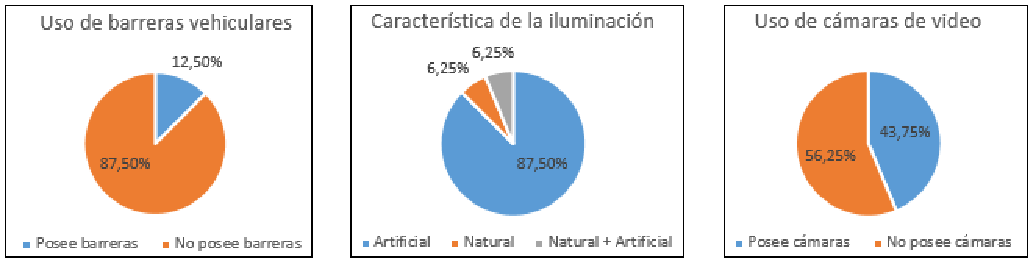
\includegraphics[width=\textwidth]{torta1-2-3a.pdf}
	\caption{Proporciones de: (a) los establecimientos que poseen y no poseen barreras, (b) de las características de la iluminación en los mismos y (c) de estacionamientos que utilizan o no cámaras de video.}
	\label{fig:img_torta1-2-3}
\end{figure}



Los estacionamientos de la ciudad que actualmente poseen cámaras de video no las utilizan para el mismo propósito que se les da en este proyecto. En la mayoría de ellos son usadas por cuestiones de seguridad, para observar la llegada de los vehículos o para ambas simultáneamente (varias cámaras con diferentes propósitos).

\subsection{Mecanismo de detección de los vehículos}
En esta sección, se presenta la forma en que se realiza la detección del vehículo en los accesos de los estacionamientos relevados. Esto se muestra en la tabla \ref{tabla:est_dec_det}, que se encuentra acompañada por el gráfico de la figura \ref{fig:img_torta4a}.

\begin{table}[h]
	\begin{center}
		\resizebox{14cm}{!} {
			\begin{tabular}{|c|c|c|c|c|} 
				\hline
				Mec. Detección & \parbox{3cm}{\centering Visualmente \\ (operador)} & \parbox{4cm}{\centering Visualmente \\
					(operador + cámaras)}
				& \parbox{3cm}{\centering Detector \\ magnético} & Botón\\
				\hline \hline
				\parbox{3cm}{\centering Proporción de \\ estacionamientos} & 62.5\% & 25\% & 6.25\% & 6.25\%\\ \hline
			\end{tabular}
		}
		\caption{Proporción de los mecanismos de detección utilizados en los estacionamientos.}
		\label{tabla:est_dec_det}
	\end{center}
\end{table}

\begin{figure}[htb]
	\centering
	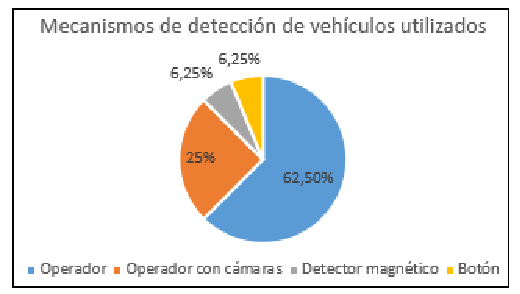
\includegraphics[scale=1]{torta4a.pdf}
	\caption{Proporciones de los tipos de mecanismos de detección de vehículos utilizados.}
	\label{fig:img_torta4a}
\end{figure}

La primera categoría hace referencia al caso en el que la detección implica que un operador se encuentra vigilando en forma visual el ingreso al establecimiento constantemente. Debido a esto, en la mayoría de los estacionamientos la cabina del operador es vidriada y se encuentra en una zona cercana a las vías de entrada-salida.

La segunda categoría se refiere a que la persona encargada de la operación del establecimiento cuenta con un sistema de cámaras apuntando hacia las vías de ingreso-egreso. Esto le permite a la misma visualizar cuando un vehículo entra o sale del establecimiento en un monitor dentro de la cabina. En este caso, esta última puede encontrarse alejada de los accesos al estacionamiento. 

La última categoría considera el uso de detectores magnéticos en los ingresos. Estos detectan la circulación de un vehículo debido a las variaciones magnéticas que el contenido ferroso de los automóviles les provoca. 

\subsection{Techo y piso}
A continuación, se muestra la proporción de estacionamientos techados y al aire libre, junto con información acerca del piso utilizado en los mismos. Esto puede observarse en las tablas \ref{tabla:est_techo} y \ref{tabla:est_piso}, que se encuentran acompañadas por los gráficos de la figura \ref{fig:img_torta5-6a}.

Debido a que se plantea un estacionamiento de prueba que sea adaptable a la mayor cantidad de escenarios posible, es importante conocer estas proporciones. Además, es necesario determinar las características del piso que generalmente se utiliza en este tipo de establecimientos. Esto se debe a que hay que asegurar que el sistema no tenga problemas con el mismo al fotografiar las chapas patentes.

\begin{table}[htbp]
	\begin{center}
		\begin{tabular}{|c|c|c|}
			\hline
			Estacionamiento techado & Sí & No\\
			\hline \hline
			Proporción de estacionamientos & 87.5\% & 12.5\% \\ \hline
		\end{tabular}
		\caption{Proporción de estacionamientos techados y al aire libre dentro de la muestra.}
		\label{tabla:est_techo}
	\end{center}
	\quad
	\begin{center}
		\begin{tabular}{|c|c|c|}
			\hline
			Tipo de piso & Cemento liso & Otro\\
			\hline \hline
			Proporción de estacionamientos & 87.5\% & 12.5\% \\ \hline
		\end{tabular}
		\caption{Proporción de estacionamientos según el tipo de piso.}
		\label{tabla:est_piso}
	\end{center}
\end{table}

\begin{figure}[htb]
	\centering
	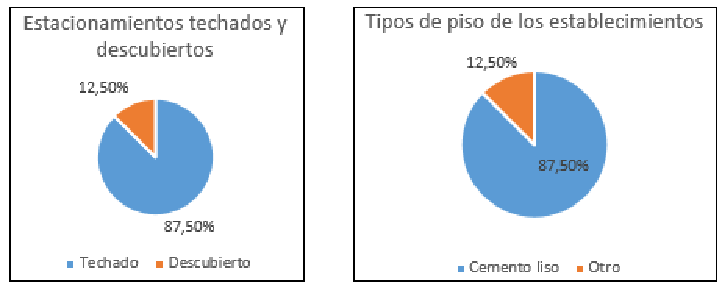
\includegraphics[scale=1]{torta5-6a.pdf}
	\caption{Proporciones de: (a) los establecimientos techados y descubiertos y (b) de los tipos de piso utilizados.}
	\label{fig:img_torta5-6a}
\end{figure}

%\begin{table}[htbp]
%	\begin{center}
%		\begin{tabular}{|c|c|c|}
%			\hline
%			Tipo de piso & Cemento liso & Otro\\
%			\hline \hline
%			Proporción de estacionamientos & 87.5\% & 12.5\% \\ \hline
%		\end{tabular}
%		\caption{Proporción de estacionamientos según el tipo de piso.}
%		\label{tabla:est_piso}
%	\end{center}
%\end{table}

Cabe destacar que en los dos establecimientos en el que el piso no es cemento liso se cuenta con un piso de tierra y uno compuesto por baldosas cerámicas blancas. Este último podría afectar a las cámaras debido a que puede reflejar la luz.

\subsection{Característica de las vías de entrada-salida}
En esta sección, se pretende determinar si existe una única vía utilizada para ambos propósitos o si existen dos rutas independientes. Es necesario conocer esta información debido a que el equipamiento del sistema para cada uno de estos casos puede que sea diferente. En la tabla \ref{tabla:est_vias} se observa el porcentaje de estacionamientos que poseen una única vía de acceso y el de establecimientos que poseen dos independientes. Además, el mismo puede visualizarse en la figura \ref{fig:img_torta7a}.
\begin{table}[htbp]
	\begin{center}
		\begin{tabular}{|c|c|c|c|}
			\hline
			\parbox{3cm}{\centering Vías de \\ ingreso-egreso} & Única & Dos independientes & Dos entradas y dos salidas\\
			\hline \hline
			\parbox{3cm}{\centering Proporción de \\ estacionamientos \\ \quad} & 62.5\% & 31.25\% & 6.25\%\\ \hline
		\end{tabular}
		\caption{Proporción de estacionamientos según el tipo de vías de acceso.}
		\label{tabla:est_vias}
	\end{center}
\end{table}

\begin{figure}[htb]
	\centering
	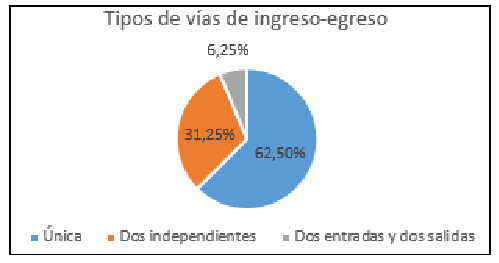
\includegraphics[scale=1]{torta7a.pdf}
	\caption{Proporciones de establecimientos que poseen una sola vía de acceso, dos vías independientes o dos vías de ingreso y dos de egreso.}
	\label{fig:img_torta7a}
\end{figure}


Existen algunos casos particulares, como es el de los establecimientos de menor nivel de afluencia de vehículos que igualmente poseen 2 vías de acceso. Al ser más pequeños, es más complicado maniobrar en el interior y suelen utilizarse ambas vías en forma indistinta. No hay una definida una ruta para la entrada y una para la salida. Igualmente, se los consideró en la categoría de “Dos independientes”. 

\subsection{Disposición del espacio en la zona de ingreso-egreso}

Esta es la característica de los establecimientos en la que mayor diversidad se encuentra. En la mayoría de los casos analizados (11) las vías de ingreso-egreso tienen forma de pasillo, de un largo que permite el acceso de uno o dos vehículos. Sin embargo, mientras que dos de ellos posibilitan la circulación de dos automóviles en paralelo, los nueve restantes se asemejan al garaje de una vivienda y solo permiten la circulación de uno. 

Por otra parte, está el caso de aquellos estacionamientos que no tienen un lugar destinado para la atención de los clientes y la misma se realiza sobre el área de ingreso. Entre los analizados se encuentran dos en esta condición. Además, se tienen establecimientos cuya entrada/salida es en forma de rampa, sobre la cual pueden ubicarse los vehículos para no esperar ser atendidos sobre la calle. En el relevamiento realizado solo hay uno correspondiente a este caso.

Finalmente, están aquellos estacionamientos que poseen más de una vía de entrada-salida, por lo que combinan algunas de las características antes mencionadas. Entre los lugares inspeccionados, se tienen dos con esta particularidad.

\section{Descripción del estacionamiento para ajustes y pruebas   }\label{key:estprotot}
En base a la investigación realizada sobre las características de los establecimientos ubicados en la ciudad de Mar del Plata se decidió simular un estacionamiento en el garaje de una casa que se tenía a disposición. Un croquis del mismo puede observarse en la figura~\ref{fig:img_croquis}.
\begin{figure}[H]
	\centering
	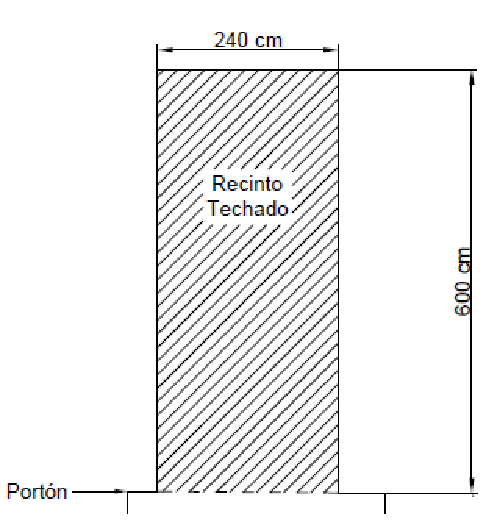
\includegraphics[scale=1]{croquis-est.pdf}
	\caption{Croquis del estacionamiento de prueba.}
	\label{fig:img_croquis}
\end{figure}

La elección realizada se fundamenta en que el establecimiento prototipo posee características similares a la de la mayoría de los que fueron inspeccionados. Las mismas se detallan a continuación:
\begin{itemize}
	\item Tiene forma de pasillo, con espacio para el ingreso de dos vehículos en fila
	\item Es techado y posee luz artificial
	\item El piso está compuesto de baldosas negras lisas. Las mismas, al igual que el piso cemento liso no afectan al momento de tomar las fotografías de la chapa patente
\end{itemize}

\hl{COSAS QUE FALTA HACER LUEGO DE COMPRAR LOS EQUIPOS Y ARMAR EL SISTEMA:}

\hl{-	Ubicacion de las camaras y demas perifericos}

\hl{-	Agregar imagenes?}




%\chapter{Primer núcleo: Reconocimiento Automático de Patentes (ALPR)} \chapterlabel{Cap_Patentes} \label{cap:alpr}

\section{Introducción}\label{sec:introALPR}
En el desarrollo del prototipo, el reconocimiento de la patente, tanto del vehículo que ingresa  como del que egresa, es una de las etapas fundamentales.

El reconocimiento automático de patentes es un problema típico que involucra varias ramas de estudio, principalmente al área de Reconocimiento de Patrones y el campo de la Visión artificial, y que ya ha sido estudiado ampliamente \cite{TRA-147} \cite{0a392c343021f65fa374375e148cb5770a88} \cite{2011-Reconocimiento_automatico_de_numero_de_patente} \cite{13EM9}.

Una de las principales dificultades que se presentan es que los escenarios pueden ser cambiantes, como podía ocurrir en el caso de un Sistema de Transporte Inteligente (ITS), donde el reconocimiento de patentes permite identificar vehículos en movimiento y obtener varias matriculas simultáneamente. \cite{0a392c343021f65fa374375e148cb5770a88} \cite{LicensePlates2018}.

En nuestro caso, a pesar de que se considera que el sistema puede aplicarse a diversos tipos de estacionamientos, el escenario es más acotado: la cámara se encuentra en una posición fija y el vehículo frenando a baja velocidad. En este contexto, se tienen en cuenta otras posibles problemáticas, como las variaciones lumínicas (día/noche), la iluminación propia de la placa y la existencia de distintos modelos de placas patentes en nuestro país: argentina antigua (1995 - 2016) y Mercosur (2016- presente). Además, se consideran diferentes tipos de vehículos: automóviles, camionetas y motocicletas.

El uso de un sistema que recoja los datos de la matrícula de un vehículo y lo almacene en una base de datos en formato de texto evita la necesidad de ocupar espacio de memoria debido al almacenamiento de videos o imágenes y facilita la consulta de los datos de cada uno de los clientes del establecimiento en el que se monte el mismo.

El objetivo de este capítulo es presentar todo lo relacionado con el desarrollo del sistema reconocedor de patentes para el Sistema Automatizado de Estacionamientos SAE. Se describen las características generales de los sistemas ALPR, los tipos de software disponibles, el sistema elegido, la parametrización e implementación del mismo, las características de los conjuntos de datos utilizados y las características principales del sistema implementado, como el tratamiento de video. 

\section{Sistemas de Reconocimiento Automático de Patentes ALPR}\label{sec:sysALPR}

\subsection{Estado del arte}
La detección de patentes de vehículos de manera automática, puede ser utilizada en varias aplicaciones como el multado de vehículos, el control de accesos y sistemas de seguridad, entre otras. Es por eso que en la actualidad existe una amplia cantidad de empresas dedicadas al reconocimiento de patentes. Entre ellas, podemos destacar a PIPS TECHNOLOGY, empresa fundada en el Reino Unido que ofrece no solo las aplicaciones previamente mencionadas, sino que además posee un sistema de transporte inteligente, control de congestionamiento, entre otras \cite{pipstechnology} . Por otra parte, se encuentra la empresa canadiense GENETEC, la cual, al igual que la anterior, ofrece soluciones de ALPR ya mencionadas como los sistemas de seguridad y el control de accesos \cite{genetec}. Por último, Neural Labs es una empresa radicada en Barcelona, España. Además de las aplicaciones ya mencionadas, la misma utiliza el reconocimiento de patentes para el control de clientes en gasolineras y peajes \cite{neurallabs}.

Particularmente en Argentina, si bien los sistemas ALPR son utilizados en algunas aplicaciones como el control de flujo o el multado, los mismos no se encuentran ampliamente difundidos, como es el caso en el plano internacional. Dentro de nuestro país, podemos mencionar la compañía VISART, la cual es una de las pocas empresas nacionales que se encuentra trabajando en el área \cite{visart}.
Además, en Argentina, aun no se han logrado grandes avances acerca del uso de sistemas ALPR en playas de estacionamiento. Por lo tanto, la implementación desarrollada en este proyecto final resulta innovadora para nuestro país.

%ALPR son las siglas en inglés del reconocimiento automático de patentes (Automatic license plate recognition). Otra manera de llamarlo es ANPR, cuyo significado es Automatic number plate recognition. El mismo consiste en la extracción de información de la patente de un vehículo a partir de una imagen. 

%Fue inventado en el año 1976 por la División de Mejora Científica de la Policía británica, pero no se popularizó hasta la década de los 90, cuando el software se hizo más sencillo de manejar y el hardware más accesible \cite{anprInt}. Actualmente, está siendo muy utilizado para diversos propósitos tales como sistemas de seguridad, estacionamientos, controles de accesos en barrios cerrados y edificios, etc. 

%Hoy en día hay una gran cantidad de herramientas disponibles que permiten realizar el reconocimiento. Las mismas pueden ser tanto “open source” (software libre) como de origen comercial. Todas estas herramientas tienen un principio de funcionamiento similar y deben ser adaptadas al lugar en el que se las pretende utilizar. Esto se debe a que las patentes de los diferentes países, estados o provincias pueden tener diferentes fuentes, colores o estar escritas en distintos idiomas. 

%Actualmente existen numerosos trabajos realizados acerca del ALPR, en los cuales cada autor lo aborda desde su perspectiva y aporta sus descubrimientos, problemáticas y resultados al investigar y experimentar  con él \hl{[ac\'a podr\'ia repetir algunas de las referencias del 2do p\'arrafo de la intro]}. 

\subsection{Etapas generales de los sistemas ALPR} \label{key:etapasgenerales}
El proceso realizado por todo sistema ALPR involucra una serie de etapas generales que pueden ser llevadas a cabo a partir de diferentes metodologías \cite{TRA-147} \cite{LicensePlates2018} \cite{UCC4791_01}. Las mismas son las que se muestran en la figura~\ref{fig:Et_gen}, y se las describe a continuación:

\begin{figure}[H]
	\centering
	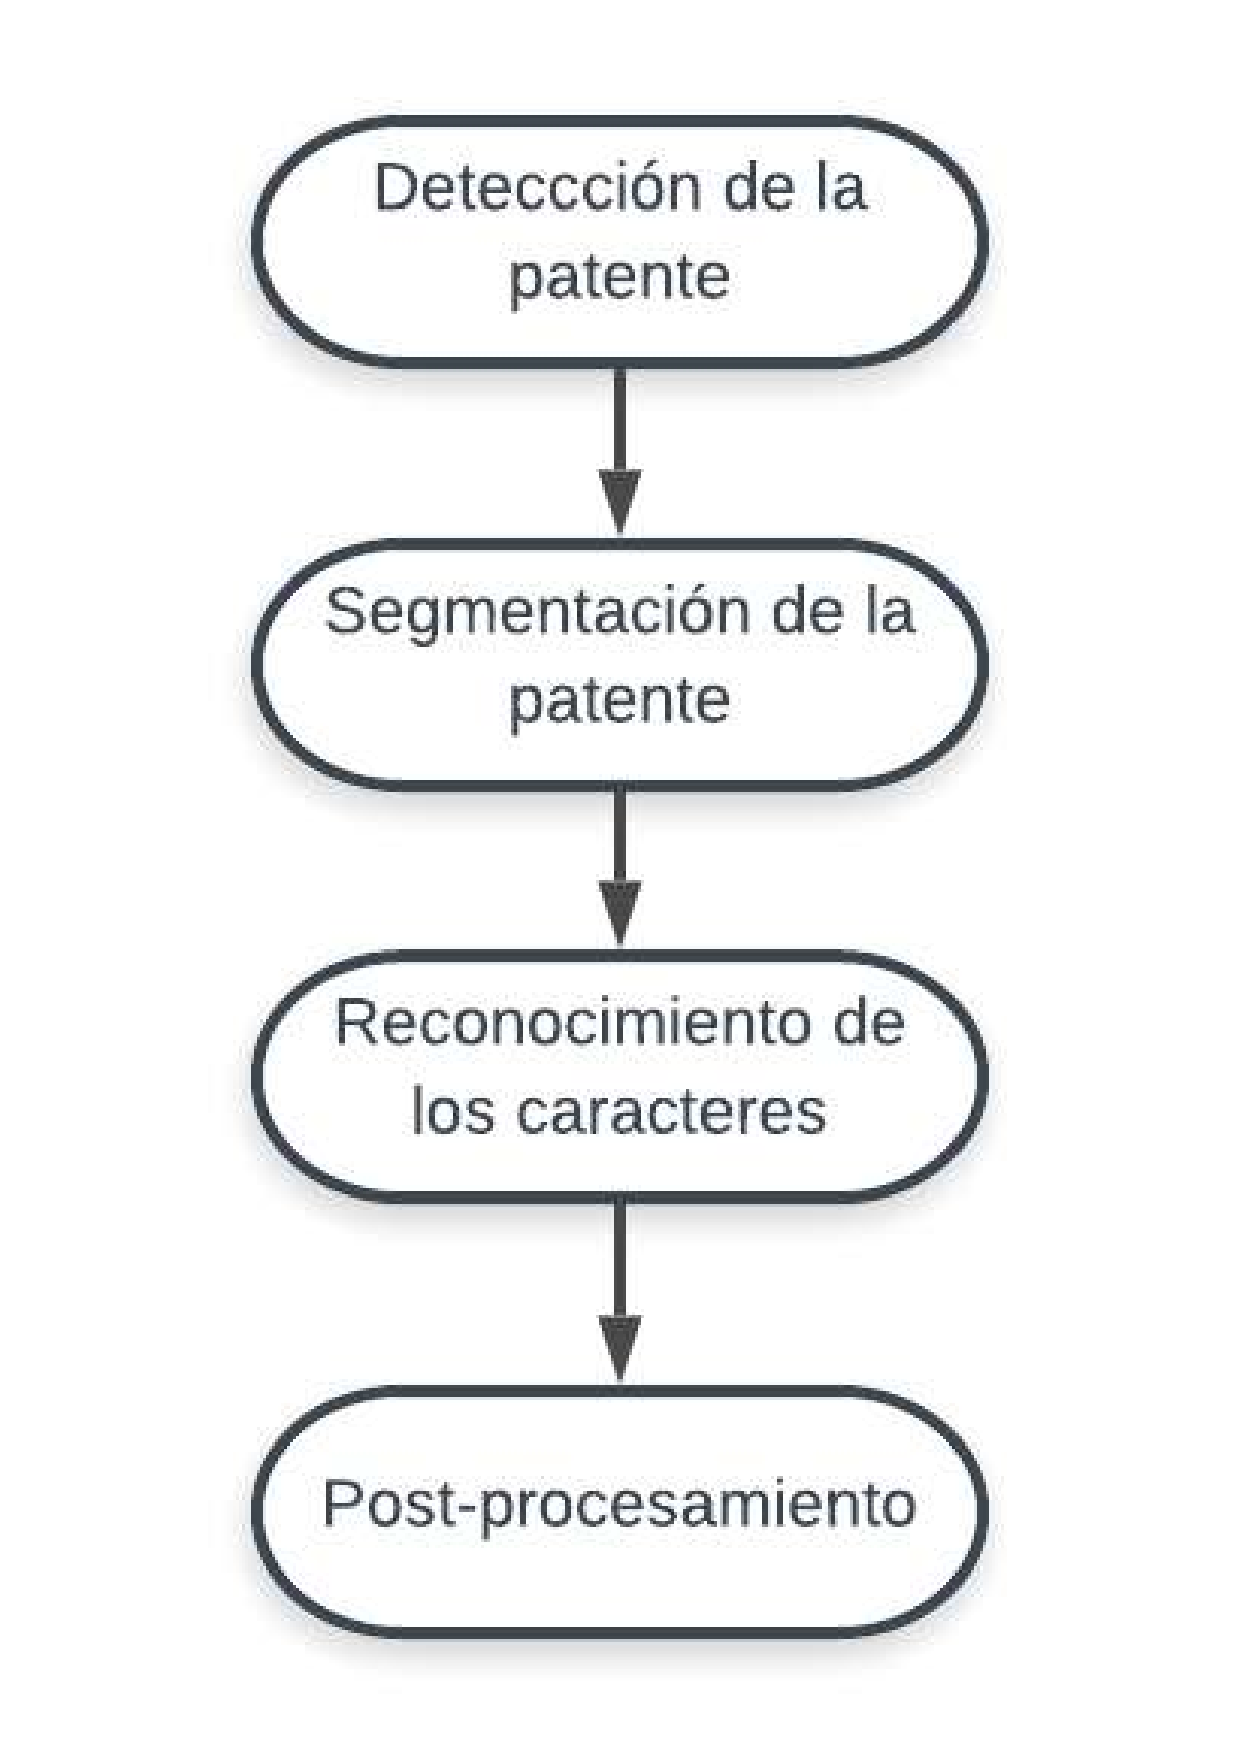
\includegraphics[scale=0.3]{Etapas_generales.pdf}
	\caption{Etapas generales de un sistema ALPR \cite{LicensePlates2018}.}
	\label{fig:Et_gen}
\end{figure} 

\noindent \textbf{Etapa 1: Detección de la patente}

Esta etapa depende en gran medida de ciertas características de la placa tales como forma, color, dimensiones, etc. Además, esta fase es afectada por las condiciones del entorno: iluminación, calidad de la cámara con la que se captura la imagen o video, las características del ambiente, etc. Normalmente, incluye una etapa de pre-procesamiento que prepara la imagen para el proceso de reconocimiento. 

El pre procesamiento consiste en la aplicación de diferentes procedimientos a la imagen, los cuales pueden variar dependiendo el algoritmo de detección que se utilice. Entre estos podemos destacar: 

\begin{itemize}
	\item \textbf{Transformación en una imagen en escala de grises:}
si la imagen a analizar se encuentra por ejemplo a color (RGB), contiene información que no es relevante, ya que el análisis de características para la identificación se realiza sobre una extracción de información acerca del valor numérico de intensidad de cada pixel y no de acuerdo al color que representa. Por lo tanto, los pixeles de la imagen transformada toman valores entre 0 y 255 pasando por las diferentes tonalidades de grises, donde 0 equivale al color negro y 255 al blanco.  Esto se observa en la figura~\ref{fig:img_grey}.

\item \textbf{Binarización:}
se realiza a través de métodos como el de Wolf Jolion \cite{wolf2004} y el de Otsu \cite{Image_Binarization_using_Otsu_Thresholdi}, entre otros. La binarización consiste en una reducción de información de una imagen digital en la que los únicos valores posibles son verdadero (1) o falso (0), los cuales corresponden a los colores blanco y negro respectivamente. Para determinar a cuál de estos valores corresponde la información de cada pixel, en el proceso de binarización se establece un umbral, que es un valor dentro de la escala de grises (0 a 255). El mismo es comparado con el valor de cada pixel y si este supera dicho umbral será un 1 y en caso contrario un 0. Además, cabe destacar, que también se pueden especificar umbrales en base a otra tonalidad, si es que se busca un objeto de un color especifico. Mediante esta técnica pueden separarse objetos o regiones que pueden ser de interés, del resto de la imagen. El resultado puede verse en la figura ~\ref{fig:img_bin}.


\item \textbf{Aplicación de filtros:}
pueden ser utilizados tanto para la remoción del ruido de la imagen como también, para realzar detalles de la misma antes de procesarla \cite{navacerrada}.
\end{itemize}

El paso siguiente es identificar la patente en la imagen, mediante algún algoritmo de detección como por ejemplo “edge detection”, “template matching” o “Artificial Neural Network” (ANN) \cite{LicensePlates2018}\cite{0a392c343021f65fa374375e148cb5770a88}. Estos algoritmos de detección, pueden combinarse con los métodos de multiescalamiento y/o ventana deslizante para encontrar la patente, independientemente del tamaño que esta posea, dentro de la imagen. 
Una vez identificada la patente en la imagen se la extrae para aplicarle una transformación a escala de grises y, luego, se la binariza con el objetivo de resaltar en blanco los caracteres y los bordes de la misma. Esto se observa en la figura~\ref{fig:img_prepro}.

\begin{figure}[H]
	\centering
	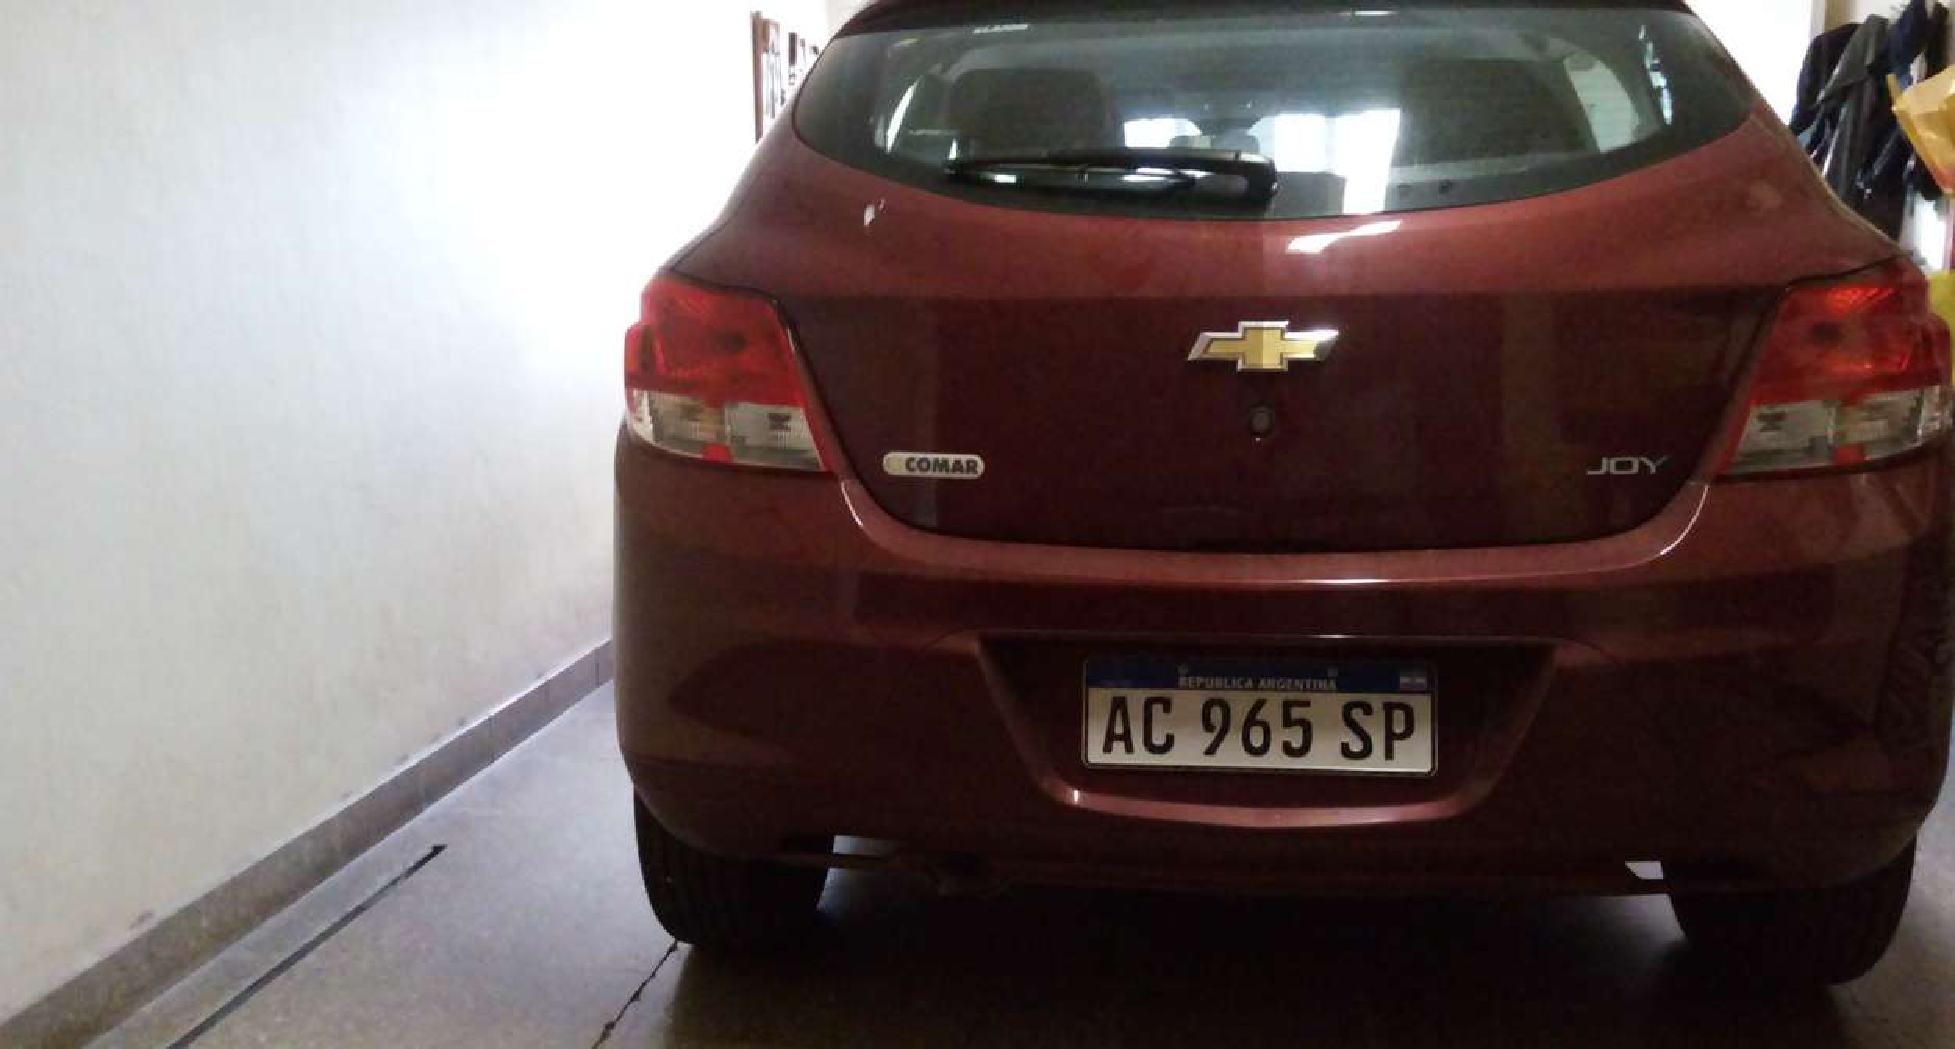
\includegraphics[scale=0.35]{imagen_original.pdf}
	\caption{Imagen del vehículo que posee la patente a analizar, antes de comenzar el proceso de reconocimiento.}
	\label{fig:img_orig}
\end{figure}
\begin{figure}[H]
	\centering
	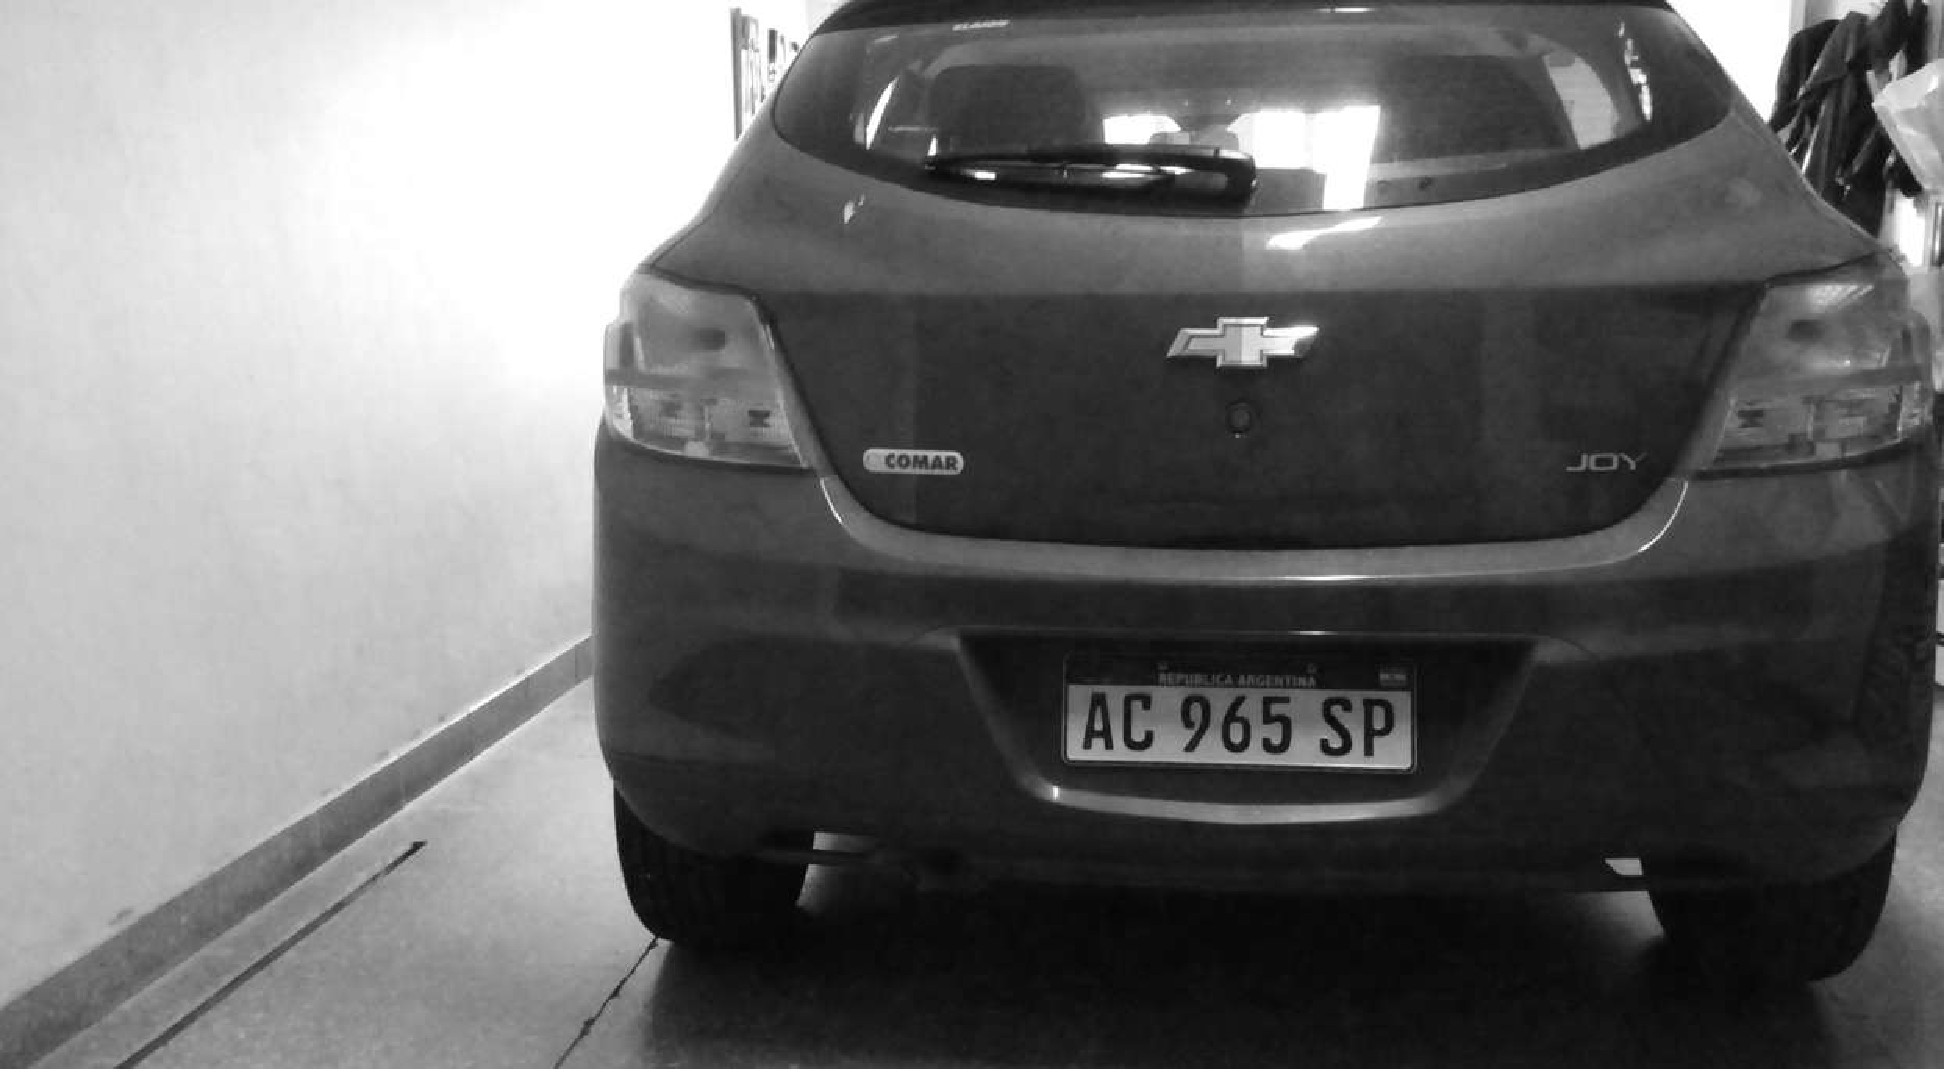
\includegraphics[scale=0.35]{escala_de_grises.pdf}
	\caption{Imagen del vehículo que posee la patente a analizar, en escala de grises.}
	\label{fig:img_grey}
\end{figure} 
\begin{figure}[H]
	\centering
	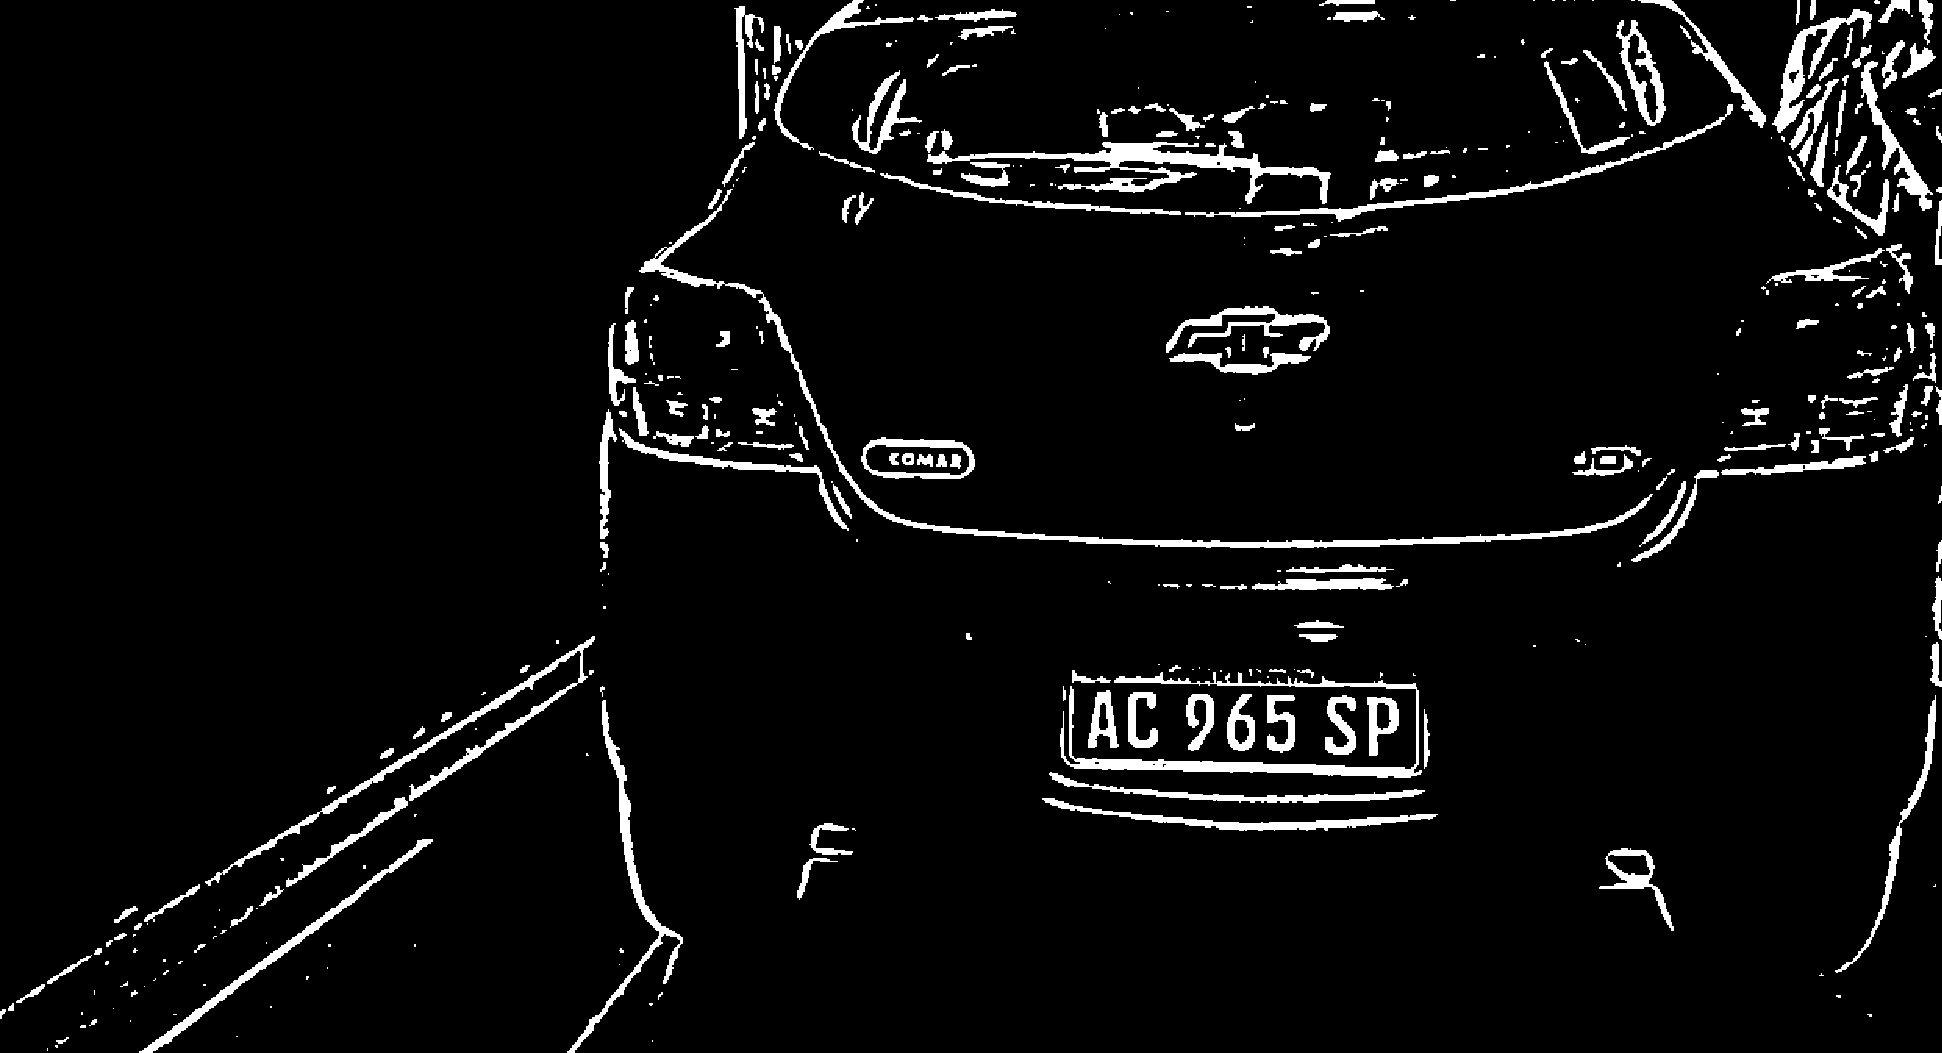
\includegraphics[scale=0.35]{imagen_binarizada.pdf}
	\caption{Imagen del vehículo que posee la patente a analizar,  luego de aplicarle el proceso de binarización.}
	\label{fig:img_bin}
\end{figure}
\begin{figure}[H]
	\centering
	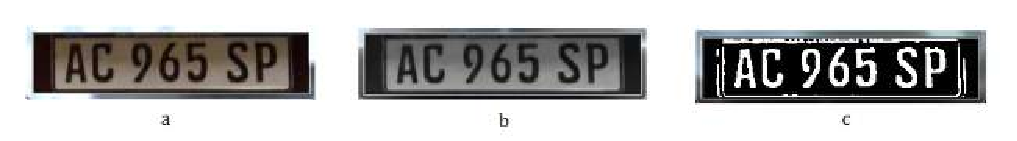
\includegraphics[width=\textwidth]{preprocesamiento_patente.pdf}
	\caption{Proceso de preprocesamiento de la región candidata: imagen original (a),  en escala de grises (b) y binarizada (c).}
	\label{fig:img_prepro}
\end{figure}


\noindent \textbf{Etapa 2: Segmentación de los caracteres de la patente}

En esta etapa, las diferentes imágenes que contienen patentes que son adquiridas por el sistema se redimensionan al mismo tamaño, de manera que el tamaño de los caracteres sea similar en todas ellas. El objetivo de esta fase es buscar las partes blancas de la imagen binarizada que cumplan con las especificaciones de los caracteres de la patente. Es por esto que en todo sistema ALPR se deben establecer algunos datos de las matriculas previamente para que el mismo quede configurado adecuadamente. Una vez que se detectan todos los caracteres de la placa, estos son aislados para luego identificarlos. El resultado del proceso de segmentación se observa en la figura~\ref{fig:img_segm}.

\begin{figure}[H]
	\centering
	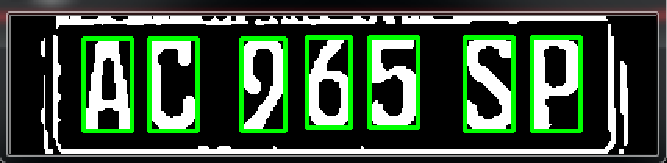
\includegraphics[scale=0.5]{segmentacion_caracteres.pdf}
	\caption{Resultado del proceso de segmentación de caracteres.}
	\label{fig:img_segm}
\end{figure}


\noindent \textbf{Etapa 3: Reconocimiento de los caracteres (OCR)}

Esta fase recibe los caracteres segmentados de la etapa anterior. Como su nombre lo indica, es la encargada de procesar cada uno de ellos y determinar a qué carácter alfanumérico corresponde. Para ello, pueden utilizarse numerosas herramientas de reconocimiento, tanto de software libre como de origen comercial, siendo la más conocida la llamada Tesseract OCR \cite{tesseractdoc}.

\quad

\noindent \textbf{Etapa 4: Post-procesamiento}

En algunos sistemas, el resultado de la etapa de reconocimiento no es solo la información obtenida del carácter analizado, sino que puede ser una lista de posibles valores con un porcentaje de confianza asociado a cada uno de ellos. En esta fase, el objetivo es tomar los resultados obtenidos y generar una lista de posibles resultados para las patentes, ordenándolas según el porcentaje de confianza. En caso de que el sistema no entregue una lista de posibilidades para los caracteres, solo se obtendrá un resultado. En la figura~\ref{fig:img_result}, se observa el resultado del proceso realizado por un sistema ALPR. Se muestra la imagen original junto con la cadena de caracteres que se corresponde con la patente.

\begin{figure}[H]
	\centering
	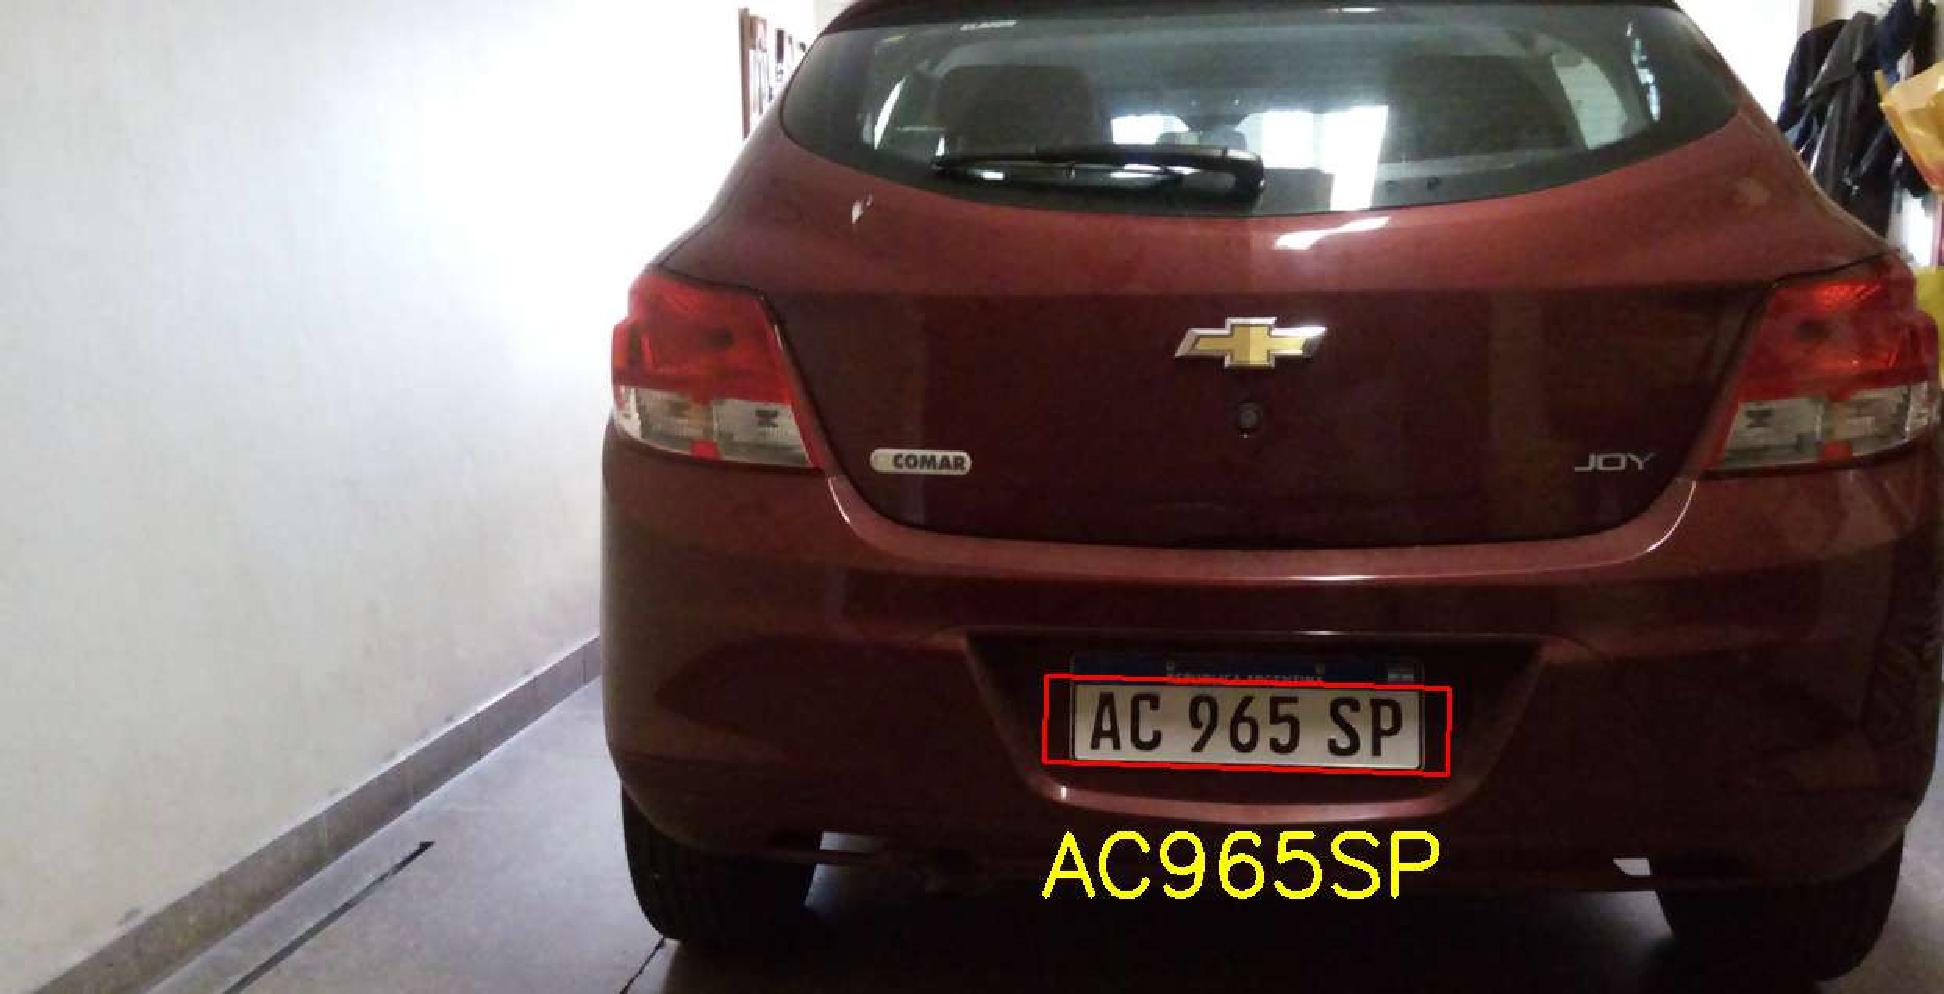
\includegraphics[scale=0.35]{resultado.pdf}
	\caption{Patente reconocida, resultante de la aplicación de un sistema ALPR.}
	\label{fig:img_result}
\end{figure}


\section{Descripción de las patentes y los conjuntos de datos}\label{sec:placpatarg}

\subsection{Patentes Argentinas} \label{key:patentesarg}

Actualmente, existen dos modelos de patentes que se encuentran en vigencia en el país \cite{Res-33-14-PATNT-MERCOSUR} \cite{caracpat1} \cite{caracpat2}.

\quad

\noindent \underline{\textbf{Patente del MERCOSUR}}

Las patentes del MERCOSUR poseen las características que pueden observarse en las figuras \ref{fig:img_pat1}, \ref{fig:img_pat2} y \ref{fig:img_pat3}, y que son listadas a continuación: 
\begin{itemize}
	\item Se implementa a partir del año 2016
	\item Está dotada de un arreglo de 7 caracteres que consta de letras y números y conforma un serial, embozado en alto relieve
	\item Elementos de seguridad que posee: 
	\begin{itemize}
		\item Bandera del país
		\item Emblema del MERCOSUR
		\item Marca de agua
		\item Tipo ensure 
		\item Estampado en caliente con lámina de seguridad con efecto difractivo y onda sinusoidal
	\end{itemize}
	\item Colores:
	\begin{itemize}
		\item Fondo de color blanco
		\item Caracteres de color negro
	\end{itemize}
	\item Dimensiones: 
	\begin{itemize}
		\item Vehículos:
		\begin{enumerate}
			\item Largo: 400mm $\pm$ 2mm
			\item Alto: 130mm $\pm$ 2mm
			\item Espesor: 1mm $\pm$ 0,2mm
		\end{enumerate}
		\item Motovehículos:
		\begin{enumerate}
			\item Largo: 200mm $\pm$  2mm
			\item Alto: 170mm $\pm$  2mm
			\item Espesor: 1mm $\pm$  0,2mm
		\end{enumerate}
	\end{itemize}
	\item Tipo de letra: 
	\begin{itemize}
		\item Fuente: FEEngschrift
		\item Alto del carácter en vehículos: 65mm 
		\item Alto del carácter en motovehículos: 53mm 
	\end{itemize}
\end{itemize}
\begin{figure}[H]
	\centering
	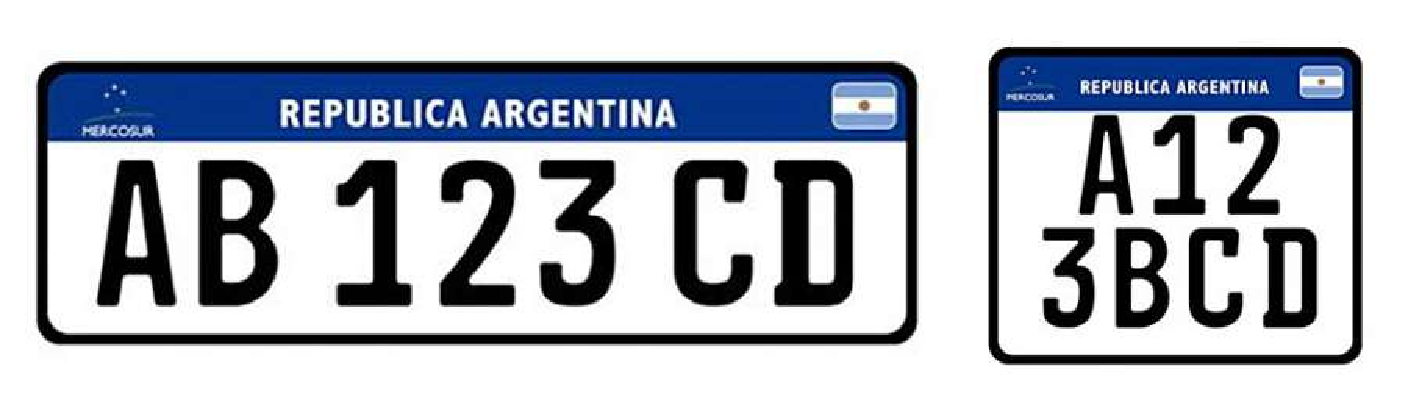
\includegraphics[scale=0.35]{pat1merc.pdf}
	\caption{Patente del MERCOSUR: características.}
	\label{fig:img_pat1}

	\quad

	\centering
	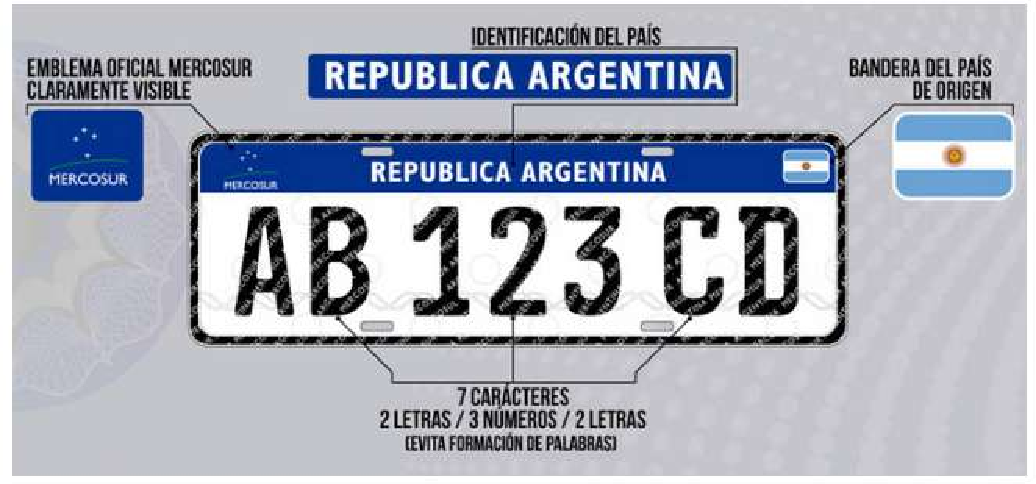
\includegraphics[scale=0.9]{pat2merc.pdf}
	\caption{Patente del MERCOSUR: medidas de seguridad.}
	\label{fig:img_pat2}
	
	\quad
	
	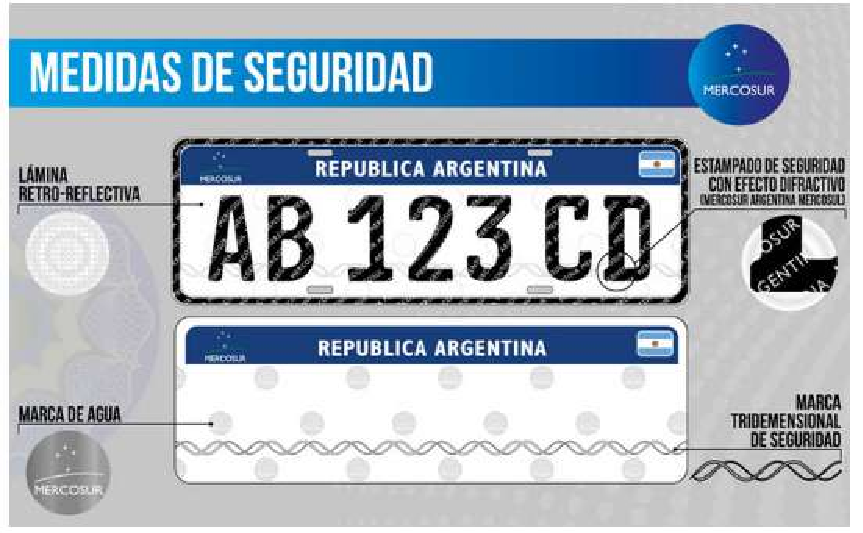
\includegraphics[scale=0.9]{pat3merc.pdf}
	\caption{Patente del MERCOSUR para automóviles y motocicletas.}
	\label{fig:img_pat3}
\end{figure}

\noindent \underline{\textbf{Patente argentina antigua}}

Las patentes antiguas poseen las características que pueden observarse en las figuras \ref{fig:img_pat1-2ant} y \ref{fig:img_pat3ant}, y que se listan a continuación: 

\begin{itemize}
	\item Se implementa entre el los años 1995 y 2016
	\item Está dotada de un arreglo de 6 caracteres que consta de letras y números y conforma un serial, embozado en bajo relieve
	\item Medidas de seguridad para evitar reproducción y/o adulteración que posee:
	\begin{itemize}
		\item Material de fabricación: aluminio
		\item Escudo Nacional a color, en el extremo superior izquierdo
		\item La palabra “ARGENTINA”, impresa en su parte media superior en color celeste
		\item Sellos circulares con la inscripción “RNPA” distribuidos en forma uniforme en los extremos blancos superior e inferior, los cuales pueden visualizarse haciendo variar la incidencia de luz sobre la misma. Se encuentran indicados en la figura~\ref{fig:img_pat1-2ant} con la letra (c)
		\item En caso de extravío, robo o hurto de la chapa patente, debe solicitarse una nueva. La única diferencia entre esta y la original es que la nueva, entre las letras y los números, lleva grabado en tamaño menor, pero de igual impresión, un carácter que determina la versión de la placa. Por ejemplo, “D” es de duplicado y  “T” es de triplicado, entre otros. Se encuentra indicado en la figura~\ref{fig:img_pat1-2ant} con la letra (d)
	\end{itemize}
	\item Colores:
	\begin{itemize}
		\item Banda central de color negro mate
		\item Caracteres sobre la banda central y de color blanco
		\item Bordes superior e inferior de color blanco reflectante
	\end{itemize}
	\item Dimensiones: 
	\begin{itemize}
		\item Vehículos:
		\begin{enumerate}
			\item Largo: 294mm 
			\item Alto: 129mm 
		\end{enumerate}
		\item Motovehículos:
		\begin{enumerate}
			\item Largo: 150mm 
			\item Alto: 130mm 
		\end{enumerate}
	\end{itemize}
%	\item Dimensiones: 
%	\begin{itemize}
%		\item Chapa metálica:
%		\begin{enumerate}
%			\item Largo: 294mm
%			\item Alto: 129mm
%		\end{enumerate}
%		\item Banda negra: 
%		\begin{enumerate}
%			\item Largo: 283mm
%			\item Alto: 78mm
%		\end{enumerate}
%	\end{itemize}
	\item Tipo de letra: 
	\begin{itemize}
		\item Fuente: LicensePlate 
		\item Ancho de los caracteres en vehículos: 32mm 
		\item Alto de los caracteres en vehículos: 67mm 
	\end{itemize}
\end{itemize}
\begin{figure}[H]
	\centering
	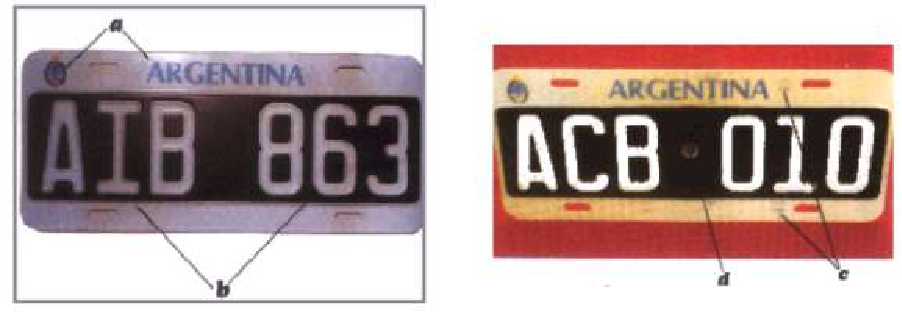
\includegraphics[width=\textwidth]{pat1-2ant.pdf}
	\caption{Patente argentina antigua correspondiente a automóviles.}
	\label{fig:img_pat1-2ant}
\end{figure}
\begin{figure}[H]
	\centering
	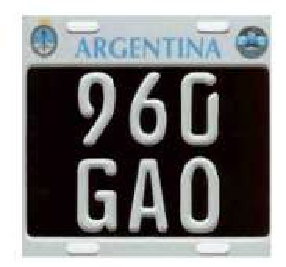
\includegraphics[scale=1]{pat3ant.pdf}
	\caption{Patente argentina antigua correspondiente a motovehículos.}
	\label{fig:img_pat3ant}
\end{figure}

A lo largo de esta sección, se plateó una numerosa lista de características correspondientes a cada uno de los modelos de patentes vigentes en nuestro país. Sin embargo, hay ciertos puntos que es necesario remarcar:
\begin{itemize}
	\item Mientras que las matrículas del MERCOSUR poseen caracteres negros sobre fondo blanco, en el modelo antiguo es a la inversa
	\item En las patentes nuevas, la letra “O” y el “0” son fácilmente diferenciables debido a que este último no se encuentra completo, debido a que posee un corte en la zona superior derecha 
	\item Respecto a las dimensiones de las mismas, el alto es similar en ambas. Sin embargo, el nuevo modelo es aproximadamente diez centímetros más ancha
	\item En cuanto a la calidad, debe mencionarse que las primeras patentes entregadas correspondientes al modelo del MERCOSUR tuvieron defectos de fabricación. Esto provocó la pérdida de pintura y el descoloramiento de las mismas \cite{fallaspat}
\end{itemize}


\subsection{Conjuntos de datos} \label{key:conjdatos}

Para probar el sistema OpenALPR y configurar sus parámetros de manera de obtener la mayor efectividad posible en su respuesta, se generaron dos conjuntos preliminares: un set de fotos para las patentes del Mercosur y otro para el modelo antiguo de matrículas argentinas. Ambos conjuntos están compuestos por 20 imágenes traseras de automóviles y camionetas. 

Esto se debe a que las motocicletas solo poseen patente en su parte trasera. Por otra parte, cabe destacar que el entorno de todas las imágenes es diferente, ya que no fueron tomadas en un mismo lugar. Por último, todas las fotos fueron tomadas con un smarthphone con una resolución de 4128 x 2322 pixeles, y luego se las re dimensionó a 1280x720 pixeles. Esta resolución se adoptó de manera de reducir el tiempo de procesamiento del sistema. La misma es configurable y admite modificaciones en caso de ser necesario. Estas imágenes fueron tomadas bajo estas condiciones, debido a que fueron pruebas preliminares y no se disponía aún de la cámara a utilizar.

Una vez finalizadas las pruebas de los diferentes parámetros del sistema, se decidió ampliar ambos sets de prueba a un tamaño de 165. Mediante estos dos nuevos conjuntos, se comprobó de mejor forma que los parámetros se hayan establecido correctamente. Las imágenes de estos sets fueron tomadas en condiciones que hacen que los mismos sean representativos del estacionamiento de prueba. Las imágenes se tomaron a distancias entre uno y cuatro metros respecto del vehículo, desde la parte trasera, a aproximadamente la altura de la matrícula, a vehículos que se encontraban detenidos y con condiciones de iluminación similares e incluso, en algunos casos, más complejas.

Por último, se crearon dos sets pequeños de 10 imágenes de motocicletas cada uno, para poder analizar el comportamiento del sistema para este tipo de vehículos.

Todos los conjuntos de imágenes establecidos, se detallan a continuación.

\subsubsection{Set de 20 imágenes de patentes del MERCOSUR}
Dentro de este conjunto, las imágenes poseen las siguientes características:
\begin{itemize}
	\item Todas las fotos son durante el día
	\item Nueve fotos fueron tomadas en línea recta a la patente y once desde un costado
	\item Se tomaron dos imágenes a un metro del vehículo, diecisiete a dos metros y una a tres metros de distancia aproximadamente
\end{itemize}

\subsubsection{Set de 20 imágenes de patentes antiguas}
Dentro de este conjunto, las imágenes poseen las siguientes características:
\begin{itemize}
	\item Todas las fotos son durante el día
	\item Once fotos fueron tomadas en línea recta a la patente y nueve desde un costado
	\item Se tomaron seis imágenes a un metro del vehículo, seis a dos metros y ocho a tres metros de distancia aproximadamente
\end{itemize}

\subsubsection{Set de 165 imágenes de patentes del MERCOSUR}
Dentro de este conjunto, las imágenes poseen las siguientes características:
\begin{itemize}
	\item Se tomaron 160 imágenes de día y 5 de noche
	\item 70 fotos fueron tomadas en línea recta a la patente y 95 desde un costado
	\item Se tomaron 33 imágenes a un metro del vehículo, 98 a dos metros, 33 a tres metros y una a cuatro metros de distancia aproximadamente
\end{itemize}

\subsubsection{Set de 165 imágenes de patentes antiguas}
Dentro de este conjunto, las imágenes poseen las siguientes características:
\begin{itemize}
	\item Se tomaron 160 imágenes de día y 5 de noche
	\item 82 fotos fueron tomadas en línea recta a la patente y 83 desde un costado
	\item Se tomaron 48 imágenes a un metro del vehículo, 90 a dos metros, 26 a tres metros y una a cuatro metros de distancia aproximadamente
\end{itemize}

\subsubsection{Set de 10 imágenes de motocicletas con patentes del MERCOSUR}
Dentro de este conjunto, las imágenes poseen las siguientes características:
\begin{itemize}
	\item Todas las fotos son durante el día
	\item 5 fotos fueron tomadas en línea recta a la patente y 5 desde un costado
	\item Se tomaron 3 imágenes a un metro del vehículo, 6 a dos metros y 1 a tres metros de distancia aproximadamente
\end{itemize}

\subsubsection{Set de 10 imágenes de motocicletas con patentes antiguas}
Dentro de este conjunto, las imágenes poseen las siguientes características:
\begin{itemize}
	\item Todas las fotos son durante el día
	\item 4 fotos fueron tomadas en línea recta a la patente y 6 desde un costado
	\item Se tomaron 4 imágenes a un metro del vehículo, 4 a dos metros y 2 a tres metros y de distancia aproximadamente
\end{itemize}


\section{Elección y ajuste del sistema para SAE}

El objetivo de esta sección, es presentar los diferentes tipos de software que se encuentran disponibles en la actualidad. Luego, se analizará el funcionamiento de dos de ellos en base a lo desarrollado en la sección \ref{key:conjdatos}, donde se explicó el funcionamiento general de un sistema ALPR. Estos sistemas fueron elegidos debido a que, al realizar una investigación sobre las herramientas disponibles, resultaron ser las que se encuentran más difundidas. Además, se expondrán los resultados de la experimentación realizada para ambos sistemas. Por último, se compararán ambos software, demostrando las razones por las que se decidió trabajar con la herramienta OpenALPR.

\subsection{Software disponibles} \label{key:implement}

Actualmente, existen numerosos trabajos realizados acerca del ALPR en los cuales cada autor lo aborda desde su perspectiva y aporta sus descubrimientos, problemáticas y resultados al investigar y experimentar con él.

Además, se tiene acceso a una gran cantidad de herramientas que permiten realizar el reconocimiento. Las mismas pueden ser sistemas pagos como “Anylines License Plate Scanner” \cite{anyline}, “Plate Recognizer” \cite{plate-recognizer} u “OpenALPR” \cite{openalpr}. En todos estos, no solo se ofrece la detección de patentes, sino que además se entregan otras funcionalidades como el almacenamiento y control en la nube, la posibilidad de integración a cualquier otro proyecto,  o bien una aplicación para smartphone, entre otras. 

Por otra parte, se pueden encontrar sistemas gratuitos, pero que no son de código abierto como lo es VISART \cite{visart}. Estos presentan la desventaja de que el proyecto se debe adaptar a lo que el software ofrece, debido a que este último no se puede modificar.

Por último, se pueden encontrar sistemas gratuitos de código abierto, entre los que podemos destacar “OpenCV 3 License Plate Recognition” \cite{opencv3}  y “OpenALPR” en su versión libre \cite{openalprfree}.

Todas estas herramientas tienen un principio de funcionamiento similar y deben ser adaptadas al lugar en el que se las pretende utilizar. Esto se debe a que las patentes de los diferentes países, estados o provincias pueden tener diversas fuentes, colores o estar escritas en distintos idiomas.

Por lo tanto, la ventaja de los sistemas pagos se encuentra en la gran variedad de países que contemplan para el reconocimiento. Pero, debido a que su uso implica una tarifa mensual o son muy costos, el desarrollo de este trabajo se focaliza en la utilización de un sistema gratuito de código abierto, el cual se busca adaptar inicialmente a las condiciones de las patentes argentinas y, a futuro, se ampliará a diferentes tipos de matrículas. Las opciones analizadas fueron ``OpenCV 3 License Plate Recognition'' y la versión libre de OpenALPR.

%Como se mencionó previamente en la sección \ref{sec:sysALPR}, hoy en día existe una gran cantidad de sistemas ALPR. Dentro de estos, se puede encontrar tanto software pago como gratuito (open source).
%En el primer grupo, se puede encontrar sistemas como “Anylines License Plate Scanner” \cite{anyline}, “Plate Recognizer” \cite{plate-recognizer} u “OpenALPR” \cite{openalpr}. En todos estos, no solo se ofrece la detección de patentes, sino que además se entregan otras funcionalidades como el almacenamiento y control en la nube, la posibilidad de integración a cualquier otro proyecto,  o bien una aplicación para smartphone, entre otras. 
%El segundo grupo está compuesto por desarrollos efectuados por terceros, como “OpenCV 3 License Plate Recognition Cpp” \cite{opencv3}, el cual es un sistema de reconocimiento de patentes basado en la librería OpenCV, realizado por Chris Dahms. Dentro de este grupo, también se puede encontrar sistemas pagos, los cuales presentan una versión de código abierto, para que diferentes desarrolladores puedan modificar el código y adaptarlo a sus necesidades, como es el caso de “OpenALPR” \cite{openalprfree}. Cabe destacar en este último caso, que este sistema no posee todas las funcionalidades de la versión comercial.
%El desarrollo de este trabajo se focalizará en la utilización de sistemas de código abierto, los cuales se buscará adaptar inicialmente a las condiciones de las patentes argentinas, y a futuro se ampliarán a diferentes tipos de matrículas. 
%En este caso, las opciones que se analizaron fueron las mencionadas anteriormente en el segundo grupo. Esto se debió a que, al realizar una investigación sobre el estado del arte, se concluyó que son las más utilizadas.

\subsection{Funcionamiento de los sistemas elegidos}\label{key:funcsistelegidos}

\subsubsection{OpenALPR}
Este es un software gratuito de código abierto, aunque también existe su versión comercial, utilizado para el reconocimiento automático de patentes de vehículos. OpenALPR está escrito en C++ y tiene la capacidad de analizar  imágenes fijas, videos y videos en tiempo real para identificar patentes en ellos y proveerla en forma de texto como salida \cite{openalprdoc}. 

Este sistema utiliza diferentes librerías para obtener el resultado, entre las que podemos destacar OpenCV \cite{libreriaopencv} para el procesamiento de la imagen y Tesseract \cite{tesseractdoc} para el reconocimiento de los caracteres.


\noindent \textbf{Etapas del sistema}	
	
Este sistema funciona bajo una arquitectura de tipo pipeline, es decir, consiste en ir transformando un flujo de datos secuencialmente a través de diferentes etapas. En este caso, la entrada del sistema es una imagen y la salida la patente del vehículo.
La documentación oficial \cite{developersguide} indica que, para obtener la respuesta, el software cuenta con 8 etapas, las cuales se comparan a continuación con las etapas generales de un sistema ALPR descriptas en la sección \ref{key:etapasgenerales}.

\quad

\noindent \textbf{Etapa 1: Detección de la patente}

Esta fase abarca las dos primeras etapas del OpenALPR que son la detección y la binarización. Esta fase funciona de la misma forma que se explicó para un sistema general, ya que se aplica un pre-procesamiento a la imagen para transformarla a escala de grises, y luego buscar la patente en dicha imagen. Para realizar esta búsqueda, el sistema utiliza un algoritmo denominado LBP (Local Binary Patterns) como algoritmo de detección.

Este es un operador de textura simple pero muy eficiente \cite{lbpalgoritmo}. Este algoritmo se encarga de extraer las características de la imagen, las cuales son lo que en visión artificial se denomina descriptores. El algoritmo, a partir de una imagen en escala de grises, calcula un valor para cada pixel de la imagen basándose en la vecindad de dicho pixel, es decir, en aquellos pixeles que lo rodean. Para hacer esto le otorga un 1 o un 0 a los pixeles de la vecindad si es que superan o no el valor del pixel central, para luego, a partir del valor binario generado, obtener el resultado LBP del pixel analizado pasando dicho valor a hexadecimal. Esto se puede observar en la figura \ref{fig:img_imagen_lbp}.

\begin{figure}[H]
	\centering
	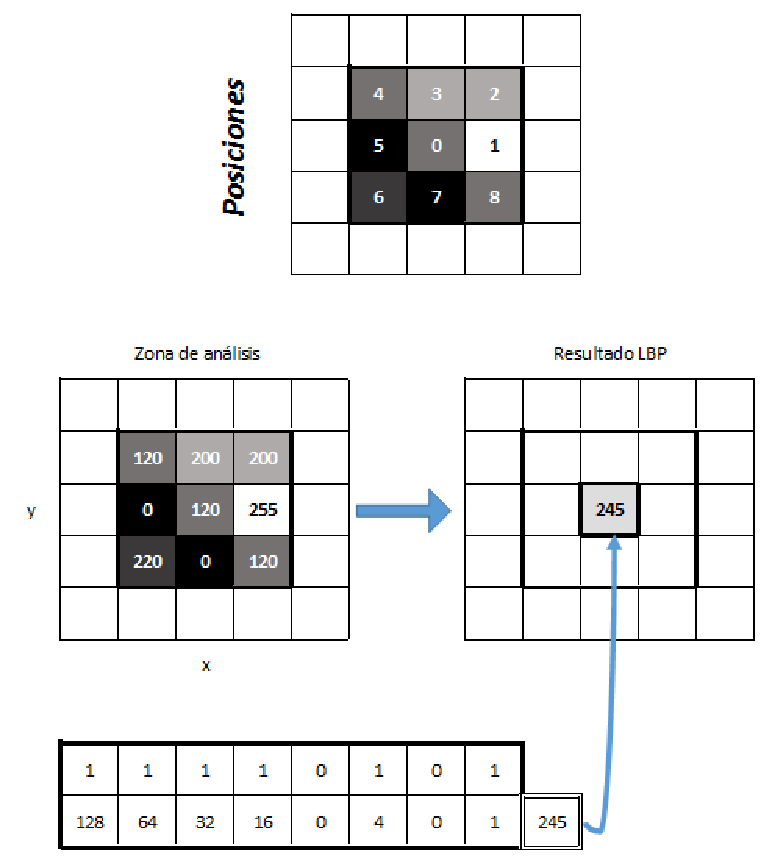
\includegraphics[scale=0.8]{imagen_lbp.pdf}
	\caption{Obtención del valor LBP de un pixel analizado \cite{imglbp}.}
	\label{fig:img_imagen_lbp}
\end{figure}

Cabe destacar que el pixel inicial puede ser cualquiera, siempre que se respete el mismo orden para todos. Luego, una vez obtenido el valor LBP para cada pixel, la parte de mayor importancia del método consiste en la generación de histogramas cuyos ejes poseen información del valor LBP de los pixeles y el porcentaje o cantidad de pixeles con ese valor.

Al obtener estos histogramas, el software OpenALPR es capaz de determinar la o las regiones donde los pixeles poseen un valor cercano a 255 (para el caso de patentes con fondo blanco) o a 0 (para patentes con fondo negro), que son los dos casos que acepta este sistema.Además, dichas regiones deben coincidir con las dimensiones preestablecidas para las patentes.

 De esta manera, el sistema es capaz de determinar la o las regiones de una o más posibles patentes en la imagen. Esto se observa en la figura \ref{fig:img_pos_pat}, donde los rectángulos de color rojo son el resultado de esta primera etapa. 	

\begin{figure}[H]
	\centering
	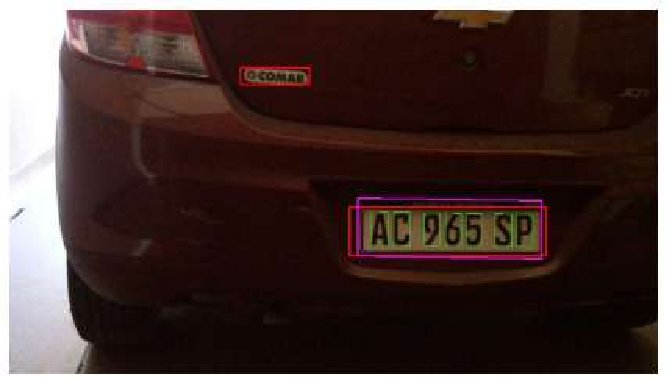
\includegraphics[scale=1]{alpr_posPat.pdf}
	\caption{Posibles patentes detectadas.}
	\label{fig:img_pos_pat}
\end{figure}

Por último, se toma un recorte de la patente de la imagen en escala de grises y se la binariza para luego ser tratada en las siguientes etapas. Cabe destacar que el sistema crea múltiples imágenes binarizadas para evitar la pérdida de un carácter en el caso de una imagen muy brillante u oscura. Para realizar la binarización, este sistema utiliza los métodos de Wolf-Jolion \cite{wolf2004} y Sauvola \cite{adaptive-document-binarization}. El método de Wolf-Jolion propone un sistema para la localización, mejora y binarización del texto en documentos multimedia. En este caso, la detección se realiza aplicando una medida de gradientes acumulados, los cuales se suelen binarizar con el método de Otsu \cite{revistaiberoamericana}. En este caso, el sistema utiliza el método Sauvola en lugar del de Otsu. El mismo aplica una ecuación de binarización de cálculo, a partir de un umbral, y utilizando la media, el nivel de desviación y la intensidad de los pixeles de la imagen. Si bien este algoritmo es más lento que el de Otsu, en imágenes con grises muy sutiles y degradados, proporciona resultados mucho más nítidos, más claros y limpios\cite{rmagro}.

\quad

\noindent \textbf{Etapa 2: Segmentación de caracteres}

 En OpenALPR esta fase abarca cuatro etapas: el análisis de caracteres, la detección de bordes de la patente, el enderezamiento y la segmentación de caracteres. En este caso, el sistema no recurre a aislar los caracteres directamente, sino que efectúa un procedimiento previo para lograr obtener mejores resultados en el reconocimiento.

En primer lugar, se buscan en las imágenes binarizadas todas las manchas que coincidan con el alto y ancho establecidos para los caracteres de la patente, tal como se observa en la figura~\ref{fig:img_det_analys}.

\begin{figure}[H]
	\centering
	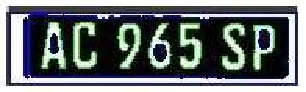
\includegraphics[scale=1]{alpr_det_analys.pdf}
	\caption{Detección y análisis de los posibles caracteres.}
	\label{fig:img_det_analys}
\end{figure}

Una vez ubicados los caracteres, se utiliza el algoritmo de Canny combinado con la transformada de Hough. Mientras el primero permite localizar contornos en la imagen, el segundo se usa para encontrar objetos en una imagen, tales como rectas, circunferencias o eclipses \cite{navacerrada}.

El objetivo de la aplicación de estos algoritmos es detectar los bordes de la patente para luego realizar el enderezamiento de la imagen y segmentar los caracteres de forma más eficiente. Este resultado, se puede observar en las figuras ~\ref{fig:img_det_bordes}(a), ~\ref{fig:img_det_bordes}(b) y ~\ref{fig:img_det_bordes}(c) donde se pueden ver las líneas ganadoras, tanto verticales como horizontales, luego de aplicar la transformada de Hough.

\begin{figure}[H]
	\centering
	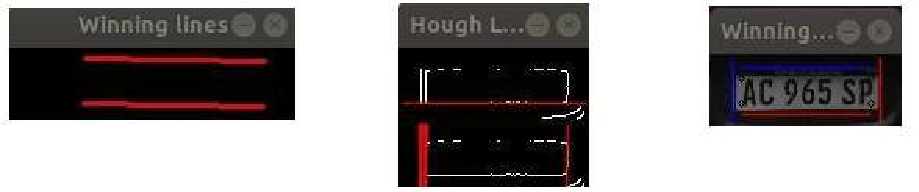
\includegraphics[width=\textwidth]{alpr_detBordes.pdf}
	\caption{Detección de bordes horizontales (a) y verticales (b), y detección de patente (c).}
	\label{fig:img_det_bordes}
\end{figure}

Por último, para segmentar los caracteres, se utiliza un histograma vertical para encontrar los espacios entre los caracteres de la patente, lo que permite leer y procesar cada carácter por separado. Además, esta etapa se encarga de limpiar los caracteres al remover puntos desconectados, descalificar regiones de caracteres por ser muy chicas e intenta remover los bordes de la patente, de manera de que no sean calificados como un “1” o una “I”. El resultado de todos estos procesos es el que se visualiza en la figura~\ref{fig:img_char_limp}.

\begin{figure}[H]
	\centering
	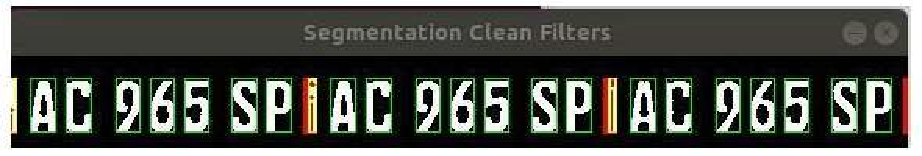
\includegraphics[width=\textwidth]{alpr_char_limp.pdf}
	\caption{Caracteres limpios y segmentados.}
	\label{fig:img_char_limp}
\end{figure}

\quad

\noindent \textbf{Etapa 3: Reconocimiento de caracteres}

Esta etapa de reconocimiento de caracteres se corresponde con la séptima etapa de OpenALPR, que lleva el mismo nombre. La misma no presenta ninguna diferencia con lo explicado en la etapa general, ya que reconoce los caracteres y, para cada uno de ellos, entrega todas las posibilidades que hay junto a un porcentaje de confianza.

Como motor de OCR, este software utiliza Tesseract. Esta herramienta se encarga, en primer lugar, de almacenar los contornos pertenecientes a los objetos de la imagen binaria que se le aporta. Luego, dichos objetos son ordenados en diferentes líneas de texto según la ubicación dentro de la imagen (coordenadas X,Y) de los contornos almacenados. Estas líneas, ahora son divididas en palabras, donde si los caracteres de esta presentan un ancho de separación fijo, cada uno de ellos se introduce en una celda de carácter. En caso contrario se divide únicamente en palabras según valores de espaciado entre ellas predefinidos.

A partir de este momento, el proceso entra en dos fases. En la primera de ellas, se hace un intento por reconocer, mediante un clasificador, cada una de las palabras (o carácter) que conforman el texto. Las que se reconocen positivamente se pasan a un clasificador adaptativo como patrón de entrenamiento, consiguiendo mayor capacidad de acierto al avanzar en el análisis del texto.

La segunda fase consiste en una nueva revisión del texto para intentar reconocer las palabras o caracteres en las que se haya fallado en la primera fase. Esto se hace debido a que el clasificado fue mejorado con los resultados positivos de la primera fase \cite{politecnicacartagena}.

Una parte de esta etapa se puede visualizar en el fragmento de la figura~\ref{fig:img_rec_char}.

\begin{figure}[H]
	\centering
	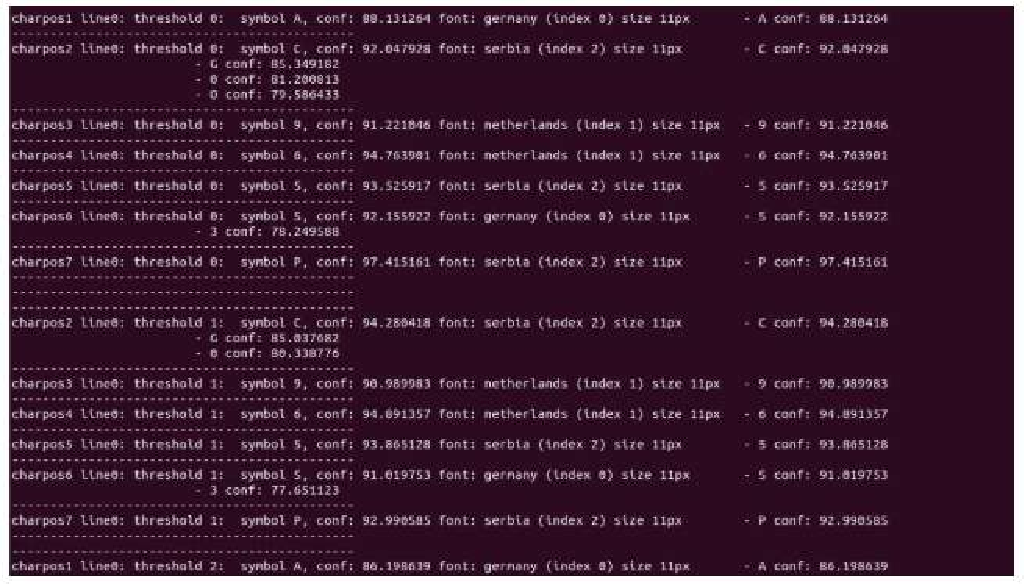
\includegraphics[width=\textwidth]{alpr_recChar.pdf}
	\caption{Fragmento del proceso de reconocimiento de los caracteres.}
	\label{fig:img_rec_char}
\end{figure}


\noindent \textbf{Etapa 4: Post-procesamiento}

Corresponde a la etapa final de este sistema y lleva el mismo nombre que la última de las etapas generales mencionada en la sección \ref{key:etapasgenerales}. En esta instancia se establece un umbral, que es un puntaje que el software calcula para el carácter basándose en la confianza y las ocurrencias de dicho carácter al reconocer los caracteres de las múltiples imágenes binarias que se generan. Entonces, si el valor resultante del carácter se encuentra por debajo del umbral, este queda rechazado como posibilidad y se lo descarta.

Luego, el sistema se encarga de determinar la mejor combinación de los resultados positivos, entregando una lista de posibles patentes ordenándolas de mejor a peor según su confianza. Esta lista, es generada a partir de permutaciones entre las posibilidades que son válidas para cada carácter. Cabe destacar que el número de patentes presente en la misma se puede seleccionar, sabiendo que no siempre se va a obtener esa cantidad máxima. 

Por último, esta etapa posee la capacidad de validar el formato de las combinaciones que se obtienen. Esto hace referencia a que se le puede decir al sistema que la patente es de determinada forma (por ejemplo: [letra][letra][letra]-[numero][numero][numero]) para que el mismo entregue solo respuestas que coincidan con dicha forma. De esta manera, se evitan las posibles confusiones entre letras y números, ya que si se reconoce un numero donde se estableció que debía haber una letra, ese resultado queda inmediatamente descartado.
El resultado final se puede observar en la figura~\ref{fig:img_postpro}. 

\begin{figure}[H]
	\centering
	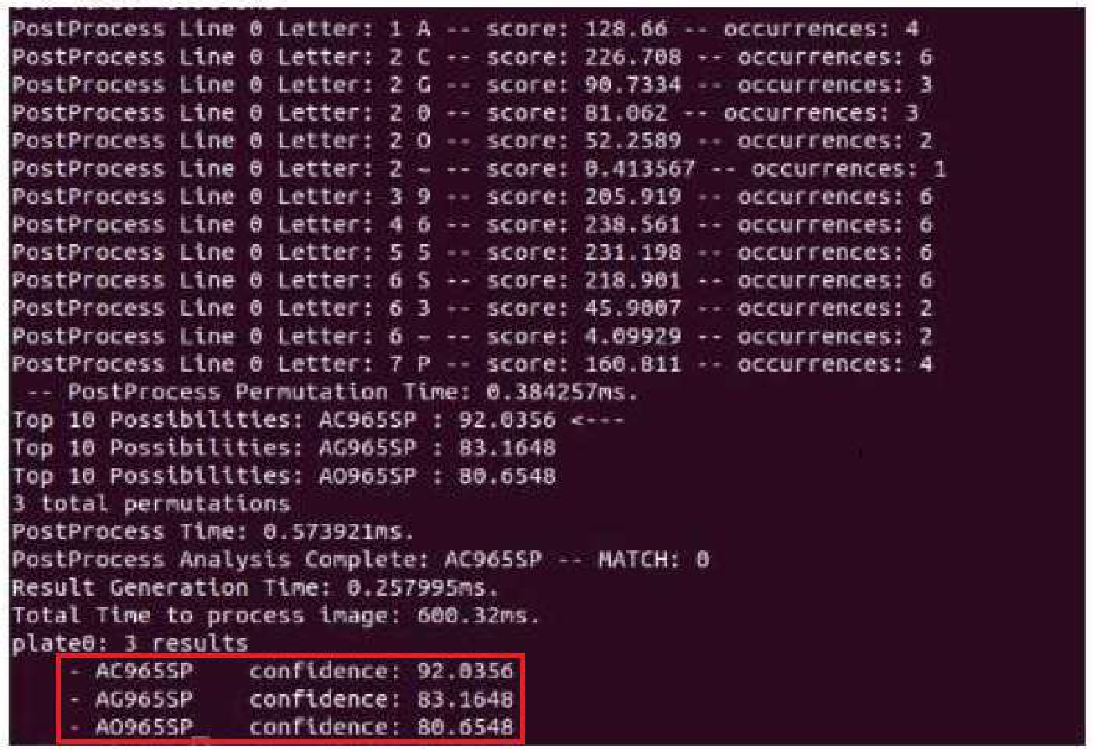
\includegraphics[width=\textwidth]{alpr_postpro.pdf}
	\caption{Fragmento de la etapa de postprocesamiento junto con el listado de patentes obtenido como resultado del proceso completo.}
	\label{fig:img_postpro}
\end{figure}


\noindent \textbf{Opciones de funcionamiento del sistema}

El software OpenALPR es capaz de reconocer matrículas a partir de tres diferentes fuentes: imágenes fijas, videos o videos en tiempo real. Cabe destacar que el proceso de obtención de la patente es idéntico para los tres casos. Esto se debe a que, en el caso de los videos, lo que se hace es analizar los diferentes frames del mismo para encontrar la patente. Es decir, el análisis se realiza a partir de una imagen que se extrae del video. 

Luego de evaluar las tres posibilidades para este proyecto, se considera más apropiado y sencillo utilizar el video en tiempo real. Esto se debe a que el sistema permanecerá continuamente analizando el video para encontrar una patente. En el caso de las imágenes fijas, primero se debería determinar el momento en que se realizaría la captura de la imagen, lo que implicaría el desarrollo de un código externo para ello. Luego, se la utilizaría para realizar el reconocimiento. Para los videos, la situación es similar. Sin embargo, se debería determinar cuándo comenzar y finalizar el video.  Además, este proceso es mucho más costoso computacionalmente y, por ende, se demora más tiempo en obtener una respuesta.

Por último, la principal ventaja de trabajar con video en lugar de imágenes fijas es que al estar continuamente analizando los frames del mismo, el sistema es capaz de entregar la respuesta para una misma patente varias veces. De esta manera, es posible obtener un resultado con mayor nivel de confianza. Para lograr esto con imágenes, se deberían obtener varias por vehículo y analizar cada una de ellas. Esto aumentaría los recursos computacionales requeridos. 

Por estos motivos, se determinó que la mejor opción es trabajar a partir del video en tiempo real. Para ello, el sistema cuenta con un modo de funcionamiento denominado alprd (alpr daemon) el cual funciona en segundo plano y permite entregarle al sistema un stream de vídeo en tiempo real.

Cuando el sistema detecta una matrícula en el vídeo, procesa el frame. A partir del mismo se obtiene el número de la patente junto con su confianza, y algunas características adicionales como el tiempo de procesamiento, la ubicación de la patente en la imagen, entre otras.

Una vez obtenida dicha información, el sistema tiene dos formas de seguir adelante. En la primera de ellas, esta es enviada a una cola de trabajo y luego a un servidor HTTP, del cual se pueden extraer los datos que contiene. La segunda forma, que es la implementada en este proyecto, es utilizando únicamente la cola de trabajo. En este caso, la misma funciona bajo el protocolo Beanstalk. Este es un protocolo que corre sobre TCP y se encarga de crear un servidor web al que el sistema sube el resultado como un nuevo trabajo o Job \cite{beanstalkprotocol}.

Para recuperar la información contenida dentro de los trabajos, es necesario extraer a estos últimos de la cola. Para ello, se usa un consumidor de cola. En este caso, para realizar esto, se desarrolló un código en C++ (podría ser en otro lenguaje) al que se añadió la librería Beanstalk-client para utilizar algunas de sus funciones con el objetivo de conectarse a este servidor, seleccionar la cola a usar, reservar un trabajo, entre otras \cite{beanstalkclient}.

Finalmente, la información recuperada se encuentra en formato “.Json”. De esta manera, a partir de un código se puede acceder fácilmente a las diferentes secciones de la misma, pero al extraer los trabajos mediante el mismo, esta pierde el formato y como resultado se obtiene una cadena de caracteres. Por lo tanto, para evitar tener que buscar la información deseada (como la patente obtenida o la confianza) en dicho texto sin formato, se dota al código de C++ de otra librería. La misma permite llevar todo ese texto al formato original (“. Json”) y trabajar con el mismo en C++ \cite{jsoncons}.

De esta manera, el sistema es capaz de obtener la información de la patente del vehículo que se ha posicionado delante de la cámara \cite{alprd}. 



\subsubsection{OpenCV 3 License Plate Recognition}
El mismo es un programa de código abierto desarrollado por Chris Damhs, el cual está implementado sobre el lenguaje C++ y está basado en la utilización de la librería OpenCV \cite{libreriaopencv}.

Este sistema tiene una estructura tipo pipeline, ya que se atraviesan diferentes etapas para lograr obtener la patente del vehículo deseado.

Respecto a la etapa general inicial de los sistemas ALPR, este software se diferencia en que, en lugar de buscar la patente en la imagen, busca primero posibles caracteres de esta para luego ubicarla. Para realizar esto, aplica en primera instancia un pre-procesamiento sobre la imagen en el que se la transforma a escala de grises y luego se la binariza mediante la función AdaptativeThresh. La misma usa binarización Gaussiana. Los resultados parciales de este proceso pueden observarse en las figuras \ref{fig:img_orig_opencv}, \ref{fig:img_escGrey_opencv} y \ref{fig:img_bin_opencv}.

\begin{figure}[H]
	\centering
	\begin{subfigure}[b]{0.49\textwidth}
		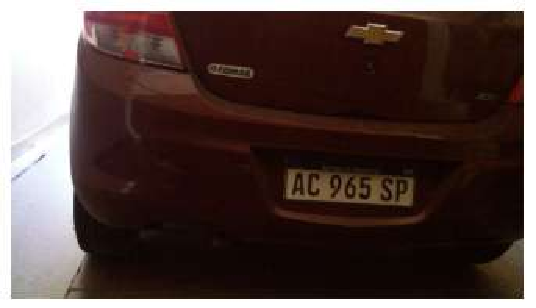
\includegraphics[width=\textwidth]{openCV_imagen_original.pdf}
		\caption{Imagen original.}
		\label{fig:img_orig_opencv}
	\end{subfigure}
	\hfill
	\begin{subfigure}[b]{0.49\textwidth}
		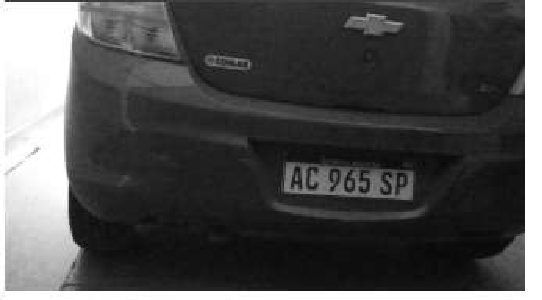
\includegraphics[width=\textwidth]{openCV_imagen_escgrises.pdf}
		\caption{Imagen en escala de grises.}
		\label{fig:img_escGrey_opencv}
	\end{subfigure}
	\hfill
	\begin{subfigure}[b]{0.49\textwidth}
		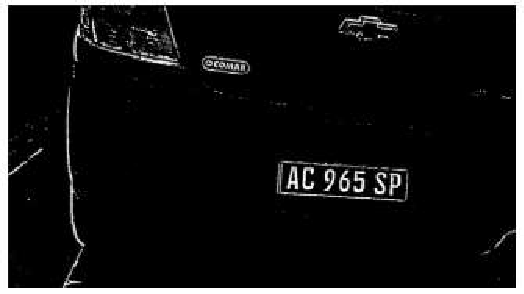
\includegraphics[width=\textwidth]{openCV_imagen_binarizada.pdf}
		\caption{Imagen binarizada.}
		\label{fig:img_bin_opencv}
	\end{subfigure}
	\caption{Resultados parciales de la etapa inicial del software basado en OpenCV.}
\end{figure}

Una vez que la imagen se encuentra binarizada se procede a buscar todos los contornos dentro de la misma. Luego, se eliminan aquellos que no coincidan con las dimensiones establecidas para los caracteres. Esto se puede observar en las figuras~\ref{fig:img_cont_opencv} y~\ref{fig:img_caract_opencv}.

\begin{figure}[H]
	\centering
	\begin{subfigure}[b]{0.49\textwidth}
		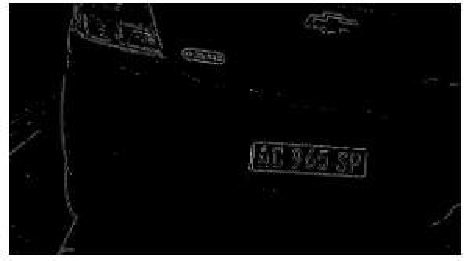
\includegraphics[scale=1]{openCV_imagen_contornos.pdf}
		\caption{Contornos dentro de la imagen binarizada.}
		\label{fig:img_cont_opencv}
	\end{subfigure}
	\hfill
	\begin{subfigure}[b]{0.49\textwidth}
		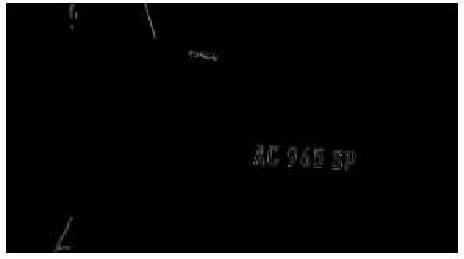
\includegraphics[scale=1]{openCV_imagen_caracteres.pdf}
		\caption{Caracteres que superaron el proceso de eliminación.}
		\label{fig:img_caract_opencv}
	\end{subfigure}
	\caption{Proceso de búsqueda de contornos y eliminación de aquellos que no poseen dimensiones de caracteres.}
\end{figure}

Con estos contornos, el sistema procede a generar diferentes grupos de caracteres, los cuales poseen características similares entre sí como el tamaño y la ubicación en las fotos. Si el grupo generado no posee un mínimo de caracteres preestablecido, queda descartado. Este resultado se observa en la figura~\ref{fig:img_caract_coinc_opencv}.

\begin{figure}[H]
	\centering
	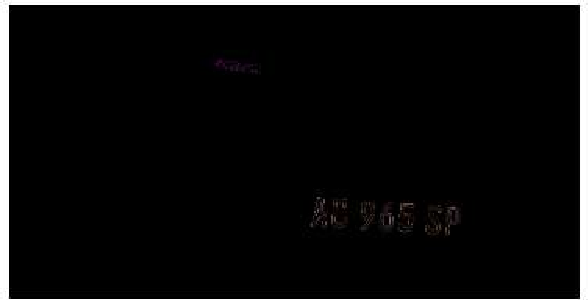
\includegraphics[scale=1]{openCV_imagen_caractCoincident.pdf}
	\caption{Grupos de caracteres coincidentes.}
	\label{fig:img_caract_coinc_opencv}
\end{figure}

Por último, basándose en la ubicación de los caracteres, el sistema los ordena y realiza un recorte de la región donde se encuentra el grupo en la imagen original. Por lo tanto, en la etapa de detección de patente, este software no entrega la ubicación de la matrícula en la imagen, sino que entrega un conjunto de posibles patentes, a las cuales se les aplica el mismo pre-procesamiento que a la imagen original, es decir, se lleva a escala de grises y se las binariza. Esto se ve en las figuras~\ref{fig:img_patente-correcta},~\ref{fig:img_patente-incorrecta} y ~\ref{fig:img_patente-luego-preproc}.

\begin{figure}[H]
	\centering
	\begin{subfigure}[b]{0.49\textwidth}
		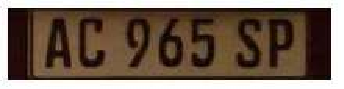
\includegraphics[width=\textwidth]{Patente-correcta.pdf}
		\caption{Patente correcta.}
		\label{fig:img_patente-correcta}
	\end{subfigure}
	\hfill
	\begin{subfigure}[b]{0.49\textwidth}
		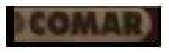
\includegraphics[width=\textwidth]{Patente-incorrecta.pdf}
		\caption{Patente incorrecta.}
		\label{fig:img_patente-incorrecta}
	\end{subfigure}
	\hfill
	\begin{subfigure}[b]{0.49\textwidth}
		
\includegraphics[scale=1]{Patente-luego-preproc.pdf}
		\caption{Patente resultante luego de aplicar el pre-procesamiento.}
		\label{fig:img_patente-luego-preproc}
	\end{subfigure}
	\caption{Proceso desarrollado en la etapa de detección de patente.}
\end{figure}

Siguiendo con el esquema general de los sistemas ALPR, esta herramienta busca segmentar los caracteres de las posibles patentes que se hayan encontrado. Para esto, realiza el mismo procedimiento utilizado para encontrar caracteres en la imagen original, pero ahora sobre la imagen de la posible patente. Una vez encontrados, mediante una comparación de tamaños y ubicación, se remueven los caracteres internos (círculo interior dentro del ``0'' o la ``O'') o superpuestos, que pueden ser considerados como un carácter diferente por sus dimensiones. De esta manera, se evita incluir dos veces el mismo carácter o caracteres extra. La figura ~\ref{fig:img_caract_remov_opencv} muestra el resultado de esta etapa.

\begin{figure}[H]
	\centering
	
\includegraphics[scale=1]{openCV_imagen_caractIntRemov.pdf}
	\caption{Resultado de la remoción de caracteres internos.}
	\label{fig:img_caract_remov_opencv}
\end{figure}

En la fase de reconocimiento de caracteres (tercera etapa general de los sistemas ALPR) este software presenta falencias ya que, en primer lugar, solo aplica el reconocimiento a la posible patente que contenga un mayor número de caracteres. Esto lo hace muy sensible a variaciones en el entorno de la imagen. En segundo lugar, utiliza el algoritmo K-NN (K Nearest Neighbours) \cite{MEMORIA-ARCEARROYO}  el cual, si bien es capaz de entregar una respuesta, no es un motor de OCR. Este es uno de los algoritmos supervisados más simples de Machine Learning, el cual se usa mayormente para la clasificación. Básicamente determina a que grupo pertenece un nuevo elemento dependiendo de cómo están clasificados sus vecinos más cercanos. Es decir, almacena todos los casos conocidos que se poseen y los utiliza para clasificar nuevos casos dependiendo de la similitud que tenga con las características determinadas \cite{navacerrada}.

Por último, se encuentra la fase de post-procesamiento. En esta, el sistema toma el resultado obtenido para cada uno de los caracteres, los cuales fueron ordenados previamente, e informa el resultado marcando con un recuadro rojo la patente seleccionada. Junto a ella, coloca los valores de los caracteres. Este último proceso se puede observar la la figura  ~\ref{fig:img_result_opencv}.

\begin{figure}[H]
	\centering
	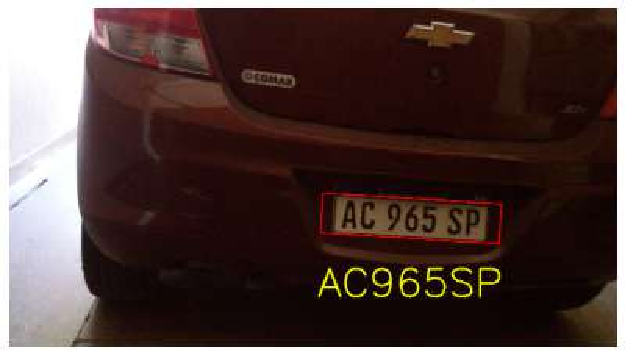
\includegraphics[scale=1]{openCV_imagen_resultado.pdf}
	\caption{Resultado entregado por la fase de post-procesamiento.}
	\label{fig:img_result_opencv}
\end{figure}	
		
		
\subsection{Experimentación y puesta a punto de los sistemas} \label{key:experimentaconypuesta}
	
En esta sección se desarrollarán las modificaciones realizadas sobre cada uno de los sistemas trabajados, con el objetivo de mejorar los resultados devueltos por ellos. Además, podrá observarse el impacto provocado por las mismas, al visualizar las respuestas obtenidas antes y después de modificar dichos sistemas. 

Para evaluar el funcionamiento de estos sistemas, se utilizó un ordenador con sistema operativo Ubuntu 18.04 LTS, un procesador Intel Core I5 de segunda generación con cuatro núcleos y 4GB de memoria RAM. 

		
\subsubsection{OpenALPR}		
		
Inicialmente, se utilizaron los sets de 20 imágenes, descritos en la sección \ref{key:conjdatos}, para evaluar el sistema con sus parámetros por defecto. Los resultados de esta prueba se muestran en la tabla \ref{tabla:openalpr_Torig}, donde en la columna ``='' se muestran las patentes reconocidas correctamente, en la columna ``X'' aquellas que fueron detectadas por el sistema con algún error en uno o más de sus caracteres y, por último, en la columna ``NF'', se encuentran las imágenes en las que el sistema no detectó ninguna patente. Esta simbología se mantendrá a lo largo de la sección de experimentación.
		
\begin{table}[htbp]
	\begin{center}
		\begin{tabular}{|c|c|c|c|}
			\hline
			& \multicolumn{3}{c|}{Set de 20 imágenes}\\
			\hline
			MERCOSUR & 75\% (15) & 10\% (2) & 15\% (3)\\
			\hline 
			Antiguas & 40\% (8) & 5\% (1) & 55\% (11)\\ \hline
		\end{tabular}
		\caption{Resultados de la detección con el entrenamiento original.}
		\label{tabla:openalpr_Torig}
	\end{center}
\end{table}		
		
Para mejorar el rendimiento de este software, fue necesario adaptarlo a las patentes argentinas. Para ello, se crearon diferentes archivos, los cuales se describen a continuación:	
		
\begin{enumerate}
	\item \textbf{\underline{Archivos de configuración de las patentes:}}
	
	A partir de lo expuesto en la sección \ref{key:patentesarg}, se crearon dos archivos de configuración (archivos de extensión ``.conf''), uno para las patentes del MERCOSUR y otro para el modelo antiguo. Dentro de estos archivos, se configuraron las dimensiones de cada una de las placas: alto, ancho, tamaño de los caracteres, entre otros. Además, se estableció la cantidad máxima y mínima de caracteres que debe poseer cada patente: 7 para modelo MERCOSUR y 6 para el antiguo. Por otra parte, el software está preparado por defecto para leer letras negras sobre un fondo blanco. Sin embargo, trabajando sobre estos archivos es posible invertir los colores de la patente para poder leer letras blancas sobre un fondo negro. Esto último se realizó únicamente en el archivo de las patentes antiguas. Adicionalmente, en estos archivos se debe configurar el entrenamiento que se aplica al motor de OCR, y el archivo del detector a utilizar. 
	
	Luego, debido a las similitudes que presentan las dimensiones de las patentes del MERCOSUR con respecto a las de las matriculas europeas, se decidió establecer estos parámetros en forma coincidente con los correspondientes a esta región, los cuales ya forman parte de la versión de código abierto de este software. En el caso del modelo antiguo ocurre algo similar con respecto a las matrículas estadounidenses, por lo que se procede de la misma forma que en el caso anterior. Por último, cabe destacar que el resto de los parámetros que se deben establecer mantuvieron los valores correspondientes a los de las matriculas europeas y estadounidenses, respectivamente.
	
	\item \textbf{\underline{Archivos de Post-Procesamiento:}}
	
	Como se mencionó en la sección \ref{key:funcsistelegidos}, el sistema es capaz de validar el formato de las combinaciones que se forman. Para realizar esto, el software utiliza, para cada estilo de patente que posee, un archivo de extensión ``.patterns'', en el cual se indica el o los formatos posibles de cada patente. Por lo tanto, se creó un archivo para las patentes del MERCOSUR donde se estableció el formato @@ \#\#\# @@, donde @ representa las letras  y \# los números. 
	
	Por otra parte, se debe destacar que en este archivo se pueden agregar los formatos del resto de las patentes del MERCOSUR, de forma de poder reconocerlas, ya que las dimensiones son las mismas. Finalmente, para las patentes argentinas antiguas se creó otro archivo en el que se estableció el formato @@@ \#\#\#.
	
	\item \textbf{\underline{Openalpr.defaults.conf:}}
	
	Es el archivo de configuración general del sistema. Contiene los parámetros por defecto establecidos en el sistema. Con el objetivo de mejorar el funcionamiento del mismo en el caso de las patentes argentinas se modificaron algunos de estos valores. Entre ellos, podemos destacar los siguientes:
	\begin{itemize}
		\item \textbf{detection\_iteration\_increase}
		
		Por defecto, este valor está establecido en 1.1.  Sin embargo, por los resultados obtenidos en la experimentación, se considera que el valor 1.07 es el que otorga mejores resultados. Cabe destacar, que este parámetro es el porcentaje de incremento del cuadro del algoritmo LBP para cada iteración, donde cuanto más bajo es su valor, más lento es el sistema.
		
		\item \textbf{must\_match\_pattern}	
		
		Este valor por defecto es 0. Su función al tomar el valor uno es informarle al sistema que las respuestas que otorgue deben coincidir con los formatos establecidos en los archivos de post-procesamiento y, en caso contrario, descartarla. Se lo seteó en 1.
		
		\item \textbf{postprocess\_min\_confidence}	
		
		Por defecto, este parámetro está establecido en 65. Este valor determina el mínimo de confianza que debe poseer cada símbolo luego de pasar por el OCR para ser considerado. Se decidió disminuirlo a 55, debido a que en este valor se obtenían una mayor cantidad de respuestas correctas que con el valor por defecto.
		
		\item \textbf{detection\_mask\_image}	
		
		Por defecto este parámetro está vacío, lo que significa que el sistema debe analizar toda la imagen en busca de la patente. Al establecer una máscara, como se observa en la figura~\ref{fig:img_mask}, el sistema solo analizará las partes blancas de la imagen e ignorará las partes negras, generando un resultado más veloz. De esta forma, se logra reducir el tiempo de procesamiento del algoritmo LBP, disminuyendo el tiempo total de procesamiento en aproximadamente 30\% con una máscara como la de la figura~\ref{fig:img_mask}. Cabe aclarar que el tiempo que se reduzca depende de la forma que posea la máscara.
		
		\begin{figure}[H]
			\centering
			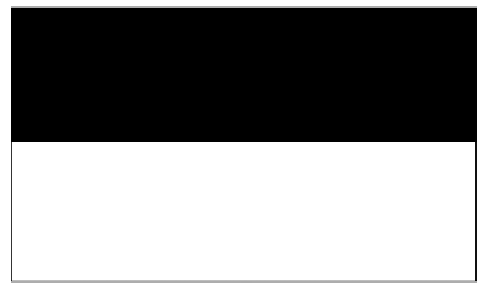
\includegraphics[scale=1]{alpr_mask.pdf}
			\caption{Ejemplo de máscara que puede ser seteada.}
			\label{fig:img_mask}
		\end{figure}
		
		\item \textbf{Prewarp} 
		
		Este parámetro permite adicionarle al software la configuración realizada sobre la cámara de video. De esta manera es posible reconocer más eficientemente las matriculas de los vehículos que no se encuentran de frente a la cámara. A pesar de que actualmente no se lo está utilizando, a futuro, este parámetro será modificado.
		
		\item \textbf{max\_plate\_width\_percent y max\_plate\_height\_percent}
		
		Por defecto, estos valores son 100. Se los seteó en 30 a ambos. De esta manera, se le informa al sistema que las posibles patentes no pueden ocupar más de un 30\% de la imagen. Por lo tanto, descartarán las posibles patentes que posean un valor superior al establecido.
		
		
	\end{itemize}
	
	\item \textbf{\underline{Archivos para el funcionamiento del ALPRD:}}
	
	Para poder ejecutar este modo de funcionamiento y reconocer las patentes argentinas, se debió modificar el archivo ``alprd.conf''. En el mismo, se le provee al sistema del URL que genera el streaming realizado por la cámara, en los parámetros ``country'' y ``pattern'' se establecen los archivos correspondientes creados para las patentes argentinas y, por último, se configura el parámetro ``topn'' en 1, ya que solo interesa obtener la mejor patente y no una lista de posibles matrículas. Además, se le configuró un ID a la cámara para poder distinguirla de las demás. 
	
	Por otro lado, como el estacionamiento considerado posee una vía de entrada y otra de salida, para que las cámaras situadas en las vías no suban sus trabajos a la misma cola de trabajo, se modificó el archivo ``daemon.cpp'' de manera que el sistema cree dos colas, una para la entrada y otra para la salida. Cabe destacar que una vez que se modifica este archivo se debe volver a compilar el software de manera que estos cambios tengan efecto sobre el funcionamiento del sistema. 
	
	Finalmente, para poder diferenciar entre las colas de entrada y salida, se debe crear un nuevo archivo ``alprd.conf'' con el ID de la cámara y el URL, referidos a las cámaras de salida. Para poder tener funcionando simultáneamente el sistema de entrada y el de salida, se debe tener una copia de los archivos ``alprd.conf'' y ``openalpr.conf'' (archivo que posee los mismos valores que openalpr.defaults.conf) para la entrada y, en una carpeta diferente, otra copia destinada a la salida, donde el ``alprd.conf'' debe estar seteado con los valores correspondientes a la salida. Por lo tanto, se deben ejecutar ambos archivos ``alprd'' en forma independiente, indicando la ubicación del archivo en el caso de que no se encuentre en la carpeta por defecto. De esta forma, las cámaras que se encuentran en la vía de entrada subirán sus trabajos a la cola de entrada y las de salida a su respectiva cola.
\end{enumerate}		
		
Una vez realizadas estas modificaciones, se volvió a evaluar el sistema utilizando los mismos sets de pruebas que al inicio, lo que permitió verificar las mejoras logradas. Los resultados se observan en la tabla \ref{tabla:openalpr_Tdesarrollado}. Cabe destacar que el parámetro detection\_iteration\_increase es el que produce el mayor impacto sobre el sistema, por lo que los nuevos resultados se presentan para tres diferentes valores de este parámetro.
		
\begin{table}[htb]
	\centering
	\resizebox{14cm}{!} {
		\begin{tabular}{|c|c|c|c|c|c|c|c|c|c|}
			\hline
			& \multicolumn{3}{c|}{1.1} & \multicolumn{3}{c|}{1.07} & \multicolumn{3}{c|}{1.04}\\
			\cline{2-10}
			& = & X & NF & = & X & NF & = & X & NF\\
			\hline \hline
			MERCOSUR & 80\% & 0\% & 20\% & 90\% & 0\% & 10\% & 90\% & 0\% & 10\%\\ \hline
			Antiguas & 70\% & 0\% & 30\% & 85\% & 0\% & 15\% & 95\% & 0\% & 5\%\\ \hline
		\end{tabular}
	}
	\caption{Variación de los resultados de los set de 20 imágenes.}
	\label{tabla:openalpr_Tdesarrollado}
\end{table}
	
Por último, se utilizaron los sets de 165 imágenes para obtener un resultado que sea más significativo. Dichos resultados se muestran el la tabla \ref{tabla:openalpr_Tdesarrollado160}.
	
\begin{table}[htb]
	\centering
	\resizebox{14cm}{!} {
		\begin{tabular}{|c|c|c|c|c|c|c|c|c|c|}
			\hline
			& \multicolumn{3}{c|}{1.1} & \multicolumn{3}{c|}{1.07} & \multicolumn{3}{c|}{1.04}\\
			\cline{2-10}
			& = & X & NF & = & X & NF & = & X & NF\\
			\hline \hline
			MERCOSUR & 92.73\% & 3.03\% & 4.24\% & 95.76\% & 0\% & 4.24\% & 95.76\% & 0\% & 4.24\%\\ \hline
			Antiguas & 88.48\% & 0.61\% & 10.91\% & 93.94\% & 0\% & 6.06\% & 94.55\% & 1.21\% & 4.24\%\\ \hline
		\end{tabular}
	}
	\caption{Resultados obtenidos para los sets de 165 imágenes.}
	\label{tabla:openalpr_Tdesarrollado160}
\end{table}	
	
Utilizando una muestra significativa de imágenes, se pudo verificar que al setear el parámetro mencionado anteriormente en 1.04 en lugar de 1.07 no se producen variaciones significativas en el reconocimiento. Mientras que en las patentes del MERCOSUR los resultados fueron los mismos que con el valor original del parámetro, en las antiguas solo hubo una mejoría de 0.61\%. Considerando que el tiempo de procesamiento es un factor muy importante y que el mismo debe ser el menor posible, se establece 1.07 como valor para el parámetro detection\_iteration\_increase.	
	
Cabe destacar que la experimentación fue realizada a partir de imágenes fijas. Sin embargo, el resultado de la misma es igualmente valido para el modo de funcionamiento a partir de un video en tiempo real debido a que procesar un frame del video es lo mismo que procesar una imagen fija.	
	
Luego de analizar el comportamiento del sistema con patentes de automóviles y camionetas se comprobó el funcionamiento del mismo con patentes de motocicletas. Este análisis se llevó a cabo sobre un número reducido de imágenes debido a que solo se buscó analizar su factibilidad, dejando a futuro el desarrollo de un conjunto de prueba mayor. Se construyeron dos sets de diez imágenes cada uno, uno con patentes del MERCOSUR y el otro con antiguas. Debe destacarse que se crearon los mismos archivos que en el caso de los otros vehículos, a excepción del archivo de configuración para las patentes del MERCOSUR. Esto se debió a que el sistema ya proveía el archivo correspondiente a las matriculas del MERCOSUR de las motos de Brasil, teniendo en cuenta que todas las matrículas del MERCOSUR son muy similares, como se mencionó anteriormente. Por último, debe mencionarse que las pruebas fueron realizadas con los parámetros de los demás archivos ya modificados, y no con los que se encontraban seteados por defecto. Los resultados obtenidos se pueden observar en la tabla \ref{tabla:pat_motos}.
	
\begin{table}[htbp]
	\begin{center}
		\begin{tabular}{|c|c|c|c|}
			\hline
			 & = & X & NF\\
			\hline 
			MERCOSUR & 100\% & 0\% & 0\%\\ 
			\hline 
			Antiguas & 90\% & 0\% & 10\%\\ \hline
		\end{tabular}
		\caption{Resultados obtenidos para el análisis de los sets con imágenes de motocicletas.}
		\label{tabla:pat_motos}
	\end{center}
\end{table}
	
	
\subsubsection{OpenCV 3 License Plate Recognition}	
	
Al igual que para el otro sistema, se realizaron las pruebas iniciales con la configuración por defecto sobre los mismos sets de 20 imágenes. En este caso, los resultados obtenidos son los observados en la tabla \ref{tabla:opencv_Torig}.	
	
\begin{table}[htb]
	\begin{center}
		\begin{tabular}{|c|c|c|c|}
			\hline
			& \multicolumn{3}{c|}{Set de 20 imágenes}\\	
			\cline{2-4}
			& = & X & NF \\
			\hline 
			MERCOSUR & 25\% & 70\% & 5\% \\ 
			\cline{1-4}
			Antiguas & 0\% & 45\% & 55\% \\ 
			\cline{1-4}
		\end{tabular}
	\caption{Resultados del reconocimiento desarrollado con la configuración por defecto.}
	\label{tabla:opencv_Torig}
	\end{center}
\end{table}		
	
Este software fue diseñado para el reconocimiento de matrículas estadounidenses, por lo que fue necesario modificarle las dimensiones de los caracteres para adaptarlos a los de las patentes argentinas. 

Por otra parte, como se mencionó previamente, para el reconocimiento de caracteres se recurre al algoritmo K-NN, el cual utiliza dos archivos: ``classification.xml'' e ``images.xml''. Los mismos son usados para entregar una respuesta para los caracteres que son analizados por el sistema. Por lo tanto, si se observan estos archivos, se puede verificar que fueron realizados para un formato de letra que no es el propio de las patentes argentina. Esto puede producir errores en el reconocimiento. En consecuencia, se desarrollaron dos nuevos archivos de cada tipo. El primer par se generó mediante una imagen que contenía todas las letras en mayúscula y todos los números con la fuente de las patentes del MERCOSUR (FEEngschrift). El segundo par se generó de la misma forma, pero con la fuente del modelo antiguo de patentes argentinas (LicensePlate).
	
Para crear dichos archivos, se utilizó el código ``OpenCV 3 KNN Character Recognition'',  basado en la librería OpenCV, desarrollado por Chris Damhs \cite{opencv3KNN}. 	Mediante el archivo ``GenData.cpp'' se pueden generar fácilmente los archivos mencionados para luego utilizarlos en el código descripto anteriormente.

Finalmente, se estableció la cantidad mínima y máxima de caracteres que debe poseer la matrícula.
	
Luego de aplicar estas modificaciones, los resultados que se obtuvieron para los mismos sets de 20 imágenes y para los nuevos de 165 son los que se muestran en la tabla \ref{tabla:opencv_Tdesarrollado}.

\begin{table}[htb]
	\centering
	\resizebox{14cm}{!} {
		\begin{tabular}{|c|c|c|c|c|c|c|}
			\hline
			& \multicolumn{3}{c|}{Set de 20 imágenes} & \multicolumn{3}{c|}{Set de 165 imágenes}\\
			\cline{2-7}
			& = & X & NF & = & X & NF\\
			\hline \hline
			MERCOSUR & 60\% & 35\% & 5\% & 37.58\% & 55.55\% & 7.87\%\\ \cline{1-7}
			Antiguas & 0\% & 45\% & 55\% & 0\% & 68.48\% & 31.52\%\\ \cline{1-7}
		\end{tabular}
	}
	\caption{Resultados de la detección con el entrenamiento desarrollado.}
	\label{tabla:opencv_Tdesarrollado}
\end{table}	
	
Cabe destacar que no se efectuó la experimentación con patentes de motocicletas con este software debido a que no posee la capacidad de entregar resultados de patentes multilinea.	
	
\subsection{Comparación de los modelos}		
	
Si bien ambos sistemas son capaces de reconocer la patente que se observa en la imagen analizada, con el software OpenALPR se logra obtener un porcentaje de éxito mayor. Esto se puede confirmar al ver los resultados obtenidos por ambos sistemas para los sets de 165 imágenes. Por un lado, en el caso de las matriculas del MERCOSUR, con el OpenALPR se obtiene una mejora del 60\% aproximadamente en el reconocimiento correcto respecto del OpenCV. Por otro lado, en el caso del modelo antiguo, se obtuvo una mejora del 95\%.

Luego de analizar el comportamiento de los sistemas, se determinó que la única ventaja que posee el código basado en OpenCV es que, al determinar primero la ubicación de los caracteres y luego la patente, este es capaz de detectar todo tipo de patentes independientemente de su tamaño. En este aspecto el software OpenALPR requiere un conjunto de archivos específicos para cada formato de matricula.

Por otra parte, OpenALPR presenta varias ventajas sobre el otro sistema que son, junto con la efectividad, las razones por las que se decidió trabajar con este software. Entre estas ventajas podemos destacar:	
	
\begin{itemize}
	\item Es más veloz
	\item Al detectar la ubicación de la patente y sus bordes, puede descartar con mayor facilidad posibles patentes
	\item Otorga una lista de posibilidades sobre la patente con un porcentaje de confianza, lo que permite detectar errores del OCR
	\item Posee la opción de invertir los colores de las patentes de manera de analizar cualquier formato bajo los mismos colores. De esta manera se evita tener que hacer un procesamiento previo de la imagen
	\item Brinda la posibilidad de validar las combinaciones de caracteres obtenidas según el formato que tengan
	\item Permite leer patentes multilínea, como es el caso de las matrículas de las motocicletas
	\item Permite el tratamiento de video y video en tiempo real, que fue la opción elegida para este proyecto
\end{itemize}	

En lo que respecta a los errores, en el caso del código de OpenCV, se debe mencionar que el sistema es muy sensible al entorno de la imagen. Cualquier cartel o conjunto de letras concatenadas que supere la longitud de caracteres de la patente va a ser considerado como la patente, ya que el sistema analiza una única posible matricula y es la que contenga la mayor cantidad de caracteres. También es posible que dentro del entorno se consideren como posibles caracteres partes del fondo de la imagen, debido a que el sistema trabaja con contornos y sus dimensiones para detectar los caracteres. Además, al no utilizar un motor de OCR propio, se producen confusiones entre los caracteres que son similares entre sí, como en el caso del ``0'', ``O'' y ``Q'' o bien ``B'' y ``8'', entre otros.	
	
Por otra parte, deben considerarse los posibles errores que se producen al trabajar con OpenALPR. En cuanto a las matrículas del MERCOSUR, se pudo identificar que los caracteres poseen escritos a lo ancho de ellos las palabras ``MERCOSUR'' y “Argentina” en color gris. Esto puede presentar grandes inconvenientes debido a que, si se logran apreciar en la imagen, al momento de reconocer los caracteres el sistema falla y no logra entregar una respuesta. Un ejemplo de este caso se presenta en las figuras \ref{fig:img_palabras_int} y ~\ref{fig:img_postsegment}.

\begin{figure}[H]
	\centering
	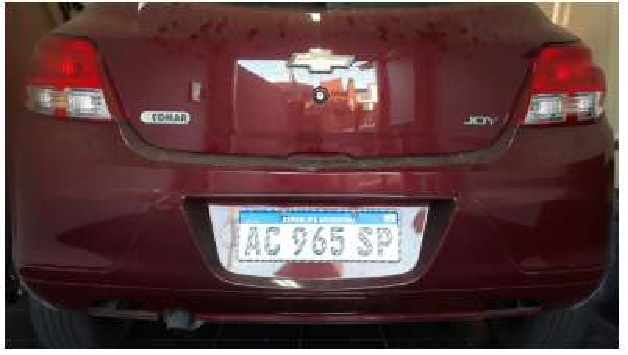
\includegraphics[scale=1]{palabras_internas.pdf}
	\caption{Patente con palabras internas apreciables.}
	\label{fig:img_palabras_int}
\end{figure}
\begin{figure}[H]
	\centering
	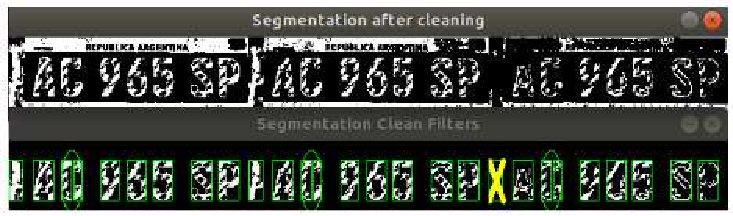
\includegraphics[scale=1]{postsegment.pdf}
	\caption{Reconocimiento de caracteres en patente con palabras internas apreciables.}
	\label{fig:img_postsegment}
\end{figure}

Como se puede observar en la figura \ref{fig:img_palabras_int}, la patente de la imagen resulta muy brillante por la forma en que la luz impacta sobre ella. Debe destacarse, en base las pruebas realizadas, que otro factor que puede influir para que esto suceda o no es el ángulo con el que se toma la imagen. Realizando variaciones sobre el mismo, se observó que el problema puede aparecer incluso si la patente no es tan brillante como se observa en el ejemplo anterior.

La solución a este problema es tomar la fotografía a una distancia entre 2.5 y 3 metros aproximadamente, dependiendo de qué tan iluminada esté la patente y el ángulo que posea la cámara. A estas distancias, si bien se siguen apreciando las palabras dentro de los caracteres, al segmentarlos e intentar reconocerlos no aparecen tan manchados como en el caso de la figura~\ref{fig:img_postsegment}, donde la imagen fue tomada a 1 metro de distancia.

Un problema que se produjo con ambos tipos de patente es la visualización de una sombra sobre la misma. Esto genera que a la hora de segmentar los caracteres aparezcan cortados y no se obtengan resultados. Cabe destacar que, trabajando a una distancia como la ya mencionada, el sistema igualmente puede fallar pero se vuelve mucho más robusto ante circunstancias como estas.

Por último, en cuanto al modelo antiguo, surgió una mayor cantidad de problemas en relación al ángulo de la cámara. Esto hace referencia a que rotaciones pequeñas pueden generar conflictos al reconocer caracteres como la ``O''y la ``Q'', debido a que en estas matrículas los mismos son muy similares. Si bien este problema también se da en las patentes del MERCOSUR con letras como la ``V'', la cual se confunde con la ``W'', y la ``M'' que se confunde con la ``H'', el mismo tiene una ocurrencia mucho menor que con el otro modelo.


\section{Conclusiones}
	
A lo largo de este capítulo se han introducido los sistemas ALPR, pasando por sus diferentes aplicaciones y empresas que los desarrollan y/o utilizan a nivel mundial. Además, se ha explicado el funcionamiento de un sistema ALPR en forma general y se ha hecho hincapié en el funcionamiento y la experimentación de dos software con los que se trabajó. A partir de estos últimos, se pude observar que no todos los sistemas ofrecen los mismos servicios y calidad, ya que presentan variaciones a la hora de llevar a cabo las etapas generales, dependiendo de la visión adoptada por la empresa o persona que los haya desarrollado. Por estos motivos, a la hora de elegir un sistema es de vital importancia analizar la aplicación en la que se lo va a utilizar, de manera de determinar el tipo de software que se requiere (pago, gratuito o de código abierto). Además, debe considerarse la forma en la que los mismos funcionan, de manera de determinar cuál de estos se adapta mejor a las necesidades. 

Se puede observar que la adaptación de un sistema ALPR para modelos de patentes que no vienen incorporadas en el sistema no es una tarea trivial, ya que se requiere la modificación y ajuste de una gran cantidad de parámetros. Además, se debe tener en cuenta la posibilidad de que el mismo no incluya los archivos de entrenamiento para el motor de OCR y el detector para el nuevo tipo de patentes. En este caso, sería necesario desarrollar dichos entrenamientos, lo cual es una tarea muy compleja. En el caso particular de este proyecto, debido a la similitud de las patentes argentinas con otros tipos de patentes, se pudieron reutilizar esos archivos entrenamientos a partir de los destinados a otros países. Sin embargo, en un futuro se debería realizar un entrenamiento propio para lograr mejores resultados para todos los modelos de patentes argentinas.






















%\chapter{Segundo núcleo: Placa I/O} \chapterlabel{2do-Nucleo} \label{cap:2do-nucleo}

\hl{FALTAN COMPLETAR ALGUNAS COSAS}

En el presente capítulo se tratarán los aspectos relacionados con el desarrollo del segundo gran núcleo del proyecto. El mismo consiste en el diseño y construcción de la placa encargada de controlar los equipos a ubicados en las zonas de ingreso y egreso del establecimiento. Se presentan los esquemas circuitales correspondientes a la fuente de alimentación y a la parte lógica de la placa. Finalmente, se analizan los diversos periféricos comerciales que se encuentran implementados en el sistema, y que son administrados por ella. 

\section{Componentes principales}
En esta primera sección se realiza un breve análisis acerca de los dos principales elementos que constituyen la placa de control. Los mismos son el microcontrolador y el módulo de comunicación WiFi. 

\subsection{Microcontrolador}
Para el reconocimiento del estado de los periféricos del sistema y el uso de dicha información para controlar la ejecución de diversas acciones se escogió el microcontrolador de 8 bits Atmega328P. El mismo es fabricado por la empresa Atmel. El microcontrolador cuenta con 28 pines, de los cuales 23 son líneas de entrada-salida programables. De ellas, 14 son digitales. De estas últimas, dos pertenecen a un puerto serial USART, utilizado para la transmisión de datos con el módulo de comunicación WiFi. Adicionalmente, se utilizan 11 pines digitales para el sensado del estado de los periféricos y la distribución de las tareas a realizar por los mismos, el control del encendido del módulo WiFi y la muestra de señales luminosas de alarma en caso de fallas \cite{atmega328p}. Finalmente, el microcontrolador requiere 5V de tensión de alimentación para funcionar correctamente. Este componente se ilustra en la imagen~\ref{fig:img_micro}.

\hl{Ver si falta mencionar alguna info importante del micro.}

\begin{figure}[H]
	\centering
	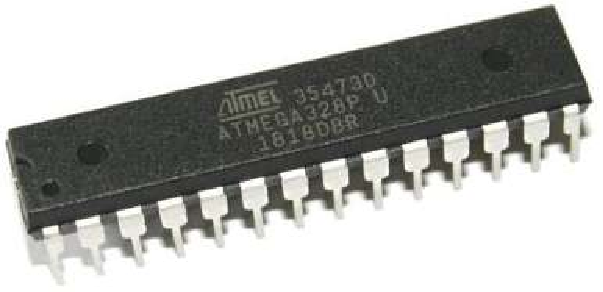
\includegraphics[scale=0.7]{micro.pdf}
	\caption{Microcontrolador Atmega328P utilizado.}
	\label{fig:img_micro}
\end{figure}


\subsection{Módulo de comunicación WiFi}

El módulo utilizado es el ESP-01, que es fabricado por Ai-Thinker y se basa en la familia de módulos WiFi “ESP8266” de Espressif Systems. El mismo se observa en la figura~\ref{fig:img_modWifi}. Este pequeño módulo puede utilizarse como adaptador Wi-Fi, que es la función que cumple en este proyecto. Mediante el mismo, se le agregó acceso inalámbrico a Internet al microcontrolador que maneja la placa, utilizando comunicación serie (USART). El módulo posee las siguientes características \cite{modwifi}:
\begin{itemize}
	\item Funciona en la banda de 2.4GHz
	\item Soporta WPA/ WPA2
	\item Rango de tensión de operación: 3 - 3.6V
	\item Consumo máximo de corriente: 170mA
	\item Puede funcionar como Estación, como Access Point (AP) o como ambas simultáneamente
\end{itemize}

Finalmente, el mismo posee ocho pines. Entre los mismos se encuentran un reset, un pin de habilitación, dos pines de alimentación y cuatro pines digitales, donde dos de ellos corresponden a una UART. En este proyecto, la UART se utiliza para la comunicación con el microcontrolador, mientras que uno de los pines digitales permite implementar una señal luminosa en caso de falla.
\begin{figure}[H]
	\centering
	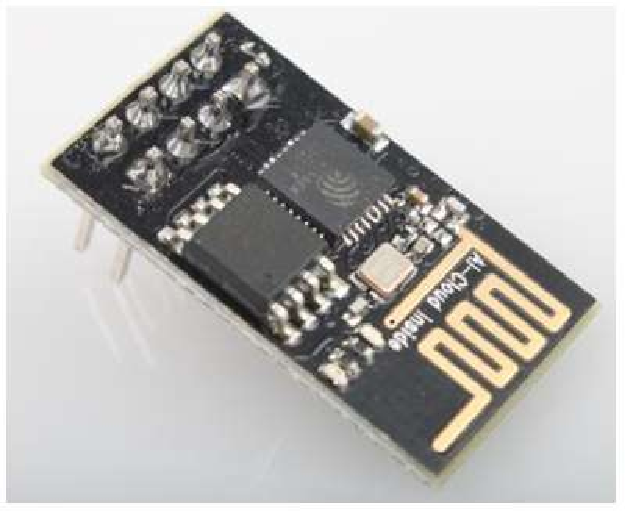
\includegraphics[scale=0.7]{modWifi.pdf}
	\caption{Módulo de comunicación  WiFi ESP-01 utilizado.}
	\label{fig:img_modWifi}
\end{figure}

\hl{ENCONTRAR Y VER SI SE ESCRIBE JUSTIFICACION SOBRE EL USO DE WIFI EN LUGAR DE OTRO PROTOCOLO. SI SE COMPLICA, SPEECH SOBRE POR QUE COSA PUEDE CAMBIARSE A FUTURO}


\section{Fuente de alimentación}
Este proyecto contempla el diseño y construcción de una fuente de tensión regulada. La misma se encarga de alimentar las barreras infrarrojas, el detector magnético, el microcontrolador y el módulo de comunicación WiFi. Para ello, cuenta con salidas de 12V, 5V y 3.3V de tensión continua. Fue implementada a partir de un transformador de 220Vac/12Vac. \textcolor{mGreen}{Su corriente de carga efectiva es X (medirla con el sistema completo conectado y funcionando).} El diagrama circuital de la fuente se observa en la figura ~\ref{fig:img_circuito_fuente}.
\begin{figure}[H]
	\centering
	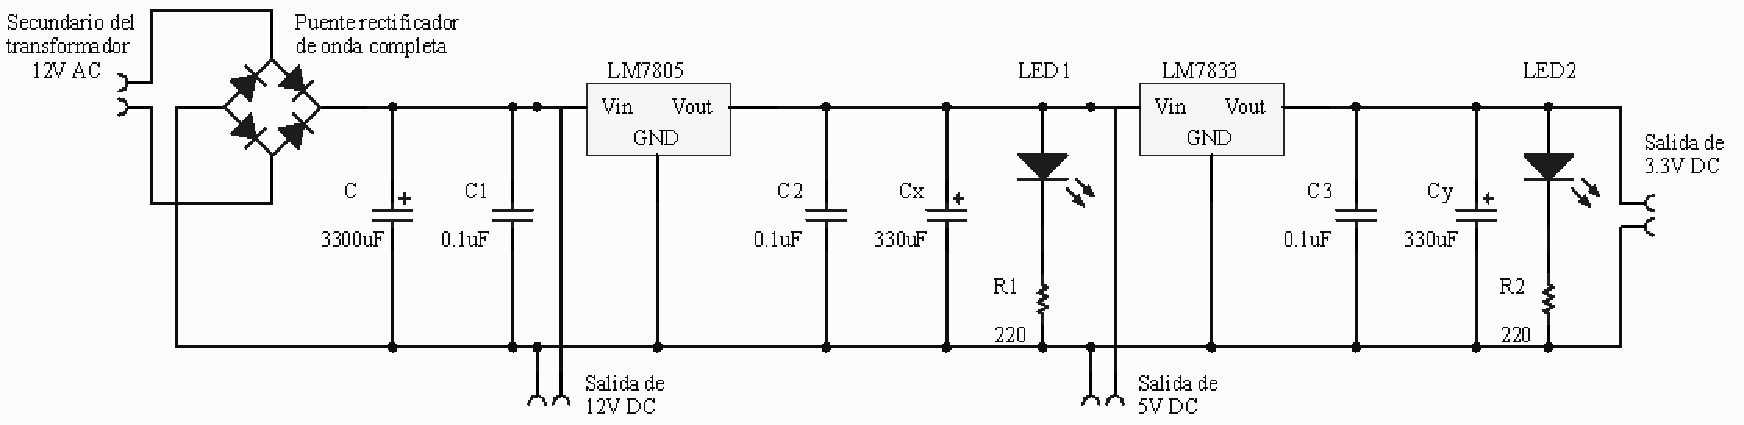
\includegraphics[width=\textwidth]{Circuito-fuente.pdf}
	\caption{Fuente de alimentación de tensión continua del sistema.}
	\label{fig:img_circuito_fuente}
\end{figure}

La fuente además cuenta con capacitores cerámicos y electrolíticos para filtrar los ruidos de alta y de baja frecuencia, respectivamente, que puedan ingresar al sistema a través de la misma, dado que se la utiliza para alimentar elementos externos, como es el caso de los periféricos (los cables actúan como antenas). 

Adicionalmente, se realizó el cálculo del disipador asociado al regulador de tensión LM7805 para que su temperatura no supere los $42^{\circ}$C. 

Finalmente, se cuenta con una protección frente a sobretensiones en el lado primario del transformador montada sobre la caja contenedora de la placa.


\section{Diseño de la etapa lógica y de comunicación}

El esquema circuital correspondiente a esta etapa se ilustra en la figura ~\ref{fig:img_circuito_logico}. Para garantizar el correcto funcionamiento del circuito básico integrado por el microcontrolador y el módulo de comunicación WiFi es necesario realizar ciertas conexiones en torno a cada uno de estos componentes.
%\textbf{OPCIÓN 2:} El esquema circuital correspondiente a esta etapa se ilustra en la figura ~\ref{fig:img_circuito_logico}. Para garantizar que el circuito básico integrado por el microcontrolador y el módulo de comunicación WiFi se encuentra en condiciones de ser encendido y comenzar a comunicarse es necesario realizar ciertas conexiones en torno a cada uno de estos componentes. 
Respecto al primero, se deben conectar las alimentaciones, un pulsador de reset y un oscilador de cristal. Este último está compuesto por un cristal de 16MHz y dos capacitores cerámicos de 22pF, como se indica en la tabla 6-3 de la hoja de datos del microcontrolador \cite{atmega328p}. El mismo es necesario para proveer al microcontrolador de una señal de reloj. En cuanto al módulo de comunicación WiFi, se debe realizar la conexión de la alimentación, el reset, el pin de habilitación y las líneas de transmisión y recepción.

\begin{figure}[H]
	\centering
	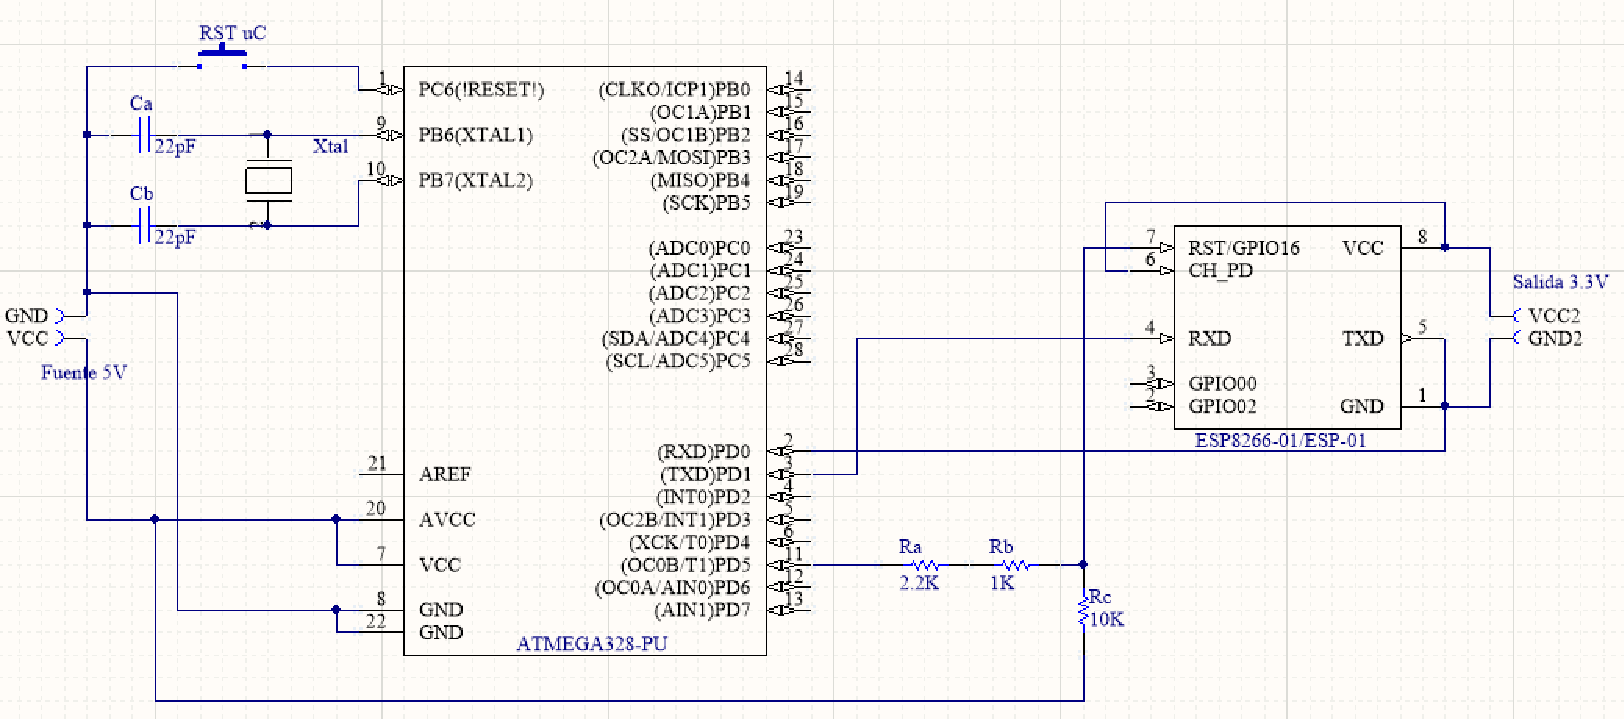
\includegraphics[width=\textwidth]{circuito-logico.pdf}
	\caption{Esquema circuital de la etapa de lógica y comunicación.}
	\label{fig:img_circuito_logico}
\end{figure}

En lo que respecta al conexionado de los periféricos que forman parte del sistema, se debe considerar el hecho de que algunos de ellos han sido simulados debido a una cuestión de costos o a que han quedado fuera del alcance del proyecto.

En cuanto a aquellos que se encuentran simulados, como es el caso de uno de los detectores magnéticos, las barreras vehiculares de entrada y salida y la expendedora de tickets del ingreso, la conexión con el microcontrolador es directa, mediante sus pines digitales de entrada. Mientras que la elevación de cada una de las barreras y la impresión del ticket se visualizan mediante un led, el segundo detector magnético y el retiro del ticket se simulan con pulsadores. 

Entre los que se encuentran verdaderamente implementados, que son las barreras infrarrojas que forman parte del sistema de detección de tamaño y uno de los sensores magnéticos de presencia, la conexión con el microcontrolador se realiza a través de una adaptación de niveles de tensión, como la de la figura~\ref{fig:img_Adapt_entradas_digitales}, para evitar dañar al mismo.

\begin{figure}[H]
	\centering
	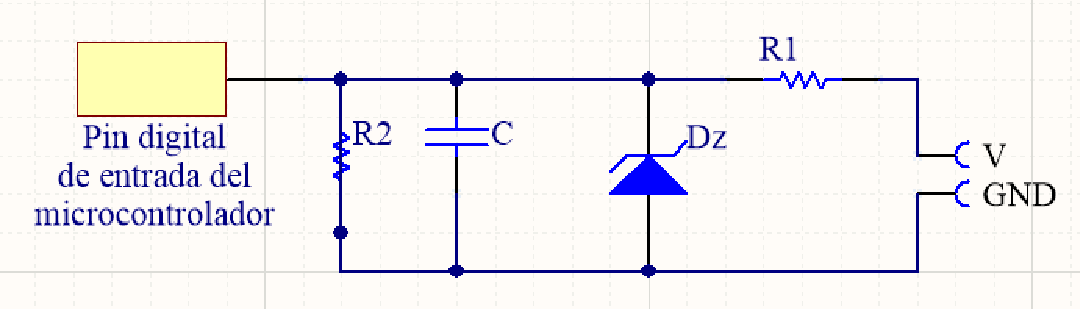
\includegraphics[width=\textwidth]{Adapt_entradas_digitales.pdf}
	\caption{Adaptación de niveles de tensión entre los periféricos y el microcontrolador.}
	\label{fig:img_Adapt_entradas_digitales}
\end{figure}

La función del diodo Zener es limitar la tensión máxima de entrada al pin digital a 5V, dado que en la hoja de datos se especifica que los mismos no admiten un valor superior a 5.5V. Esto se implementa debido a que los periféricos cuentan con contactos de relé que, en caso de cerrarse, envían al pin del microcontrolador los 12V con que son alimentados. Además, en caso de una inversión de la tensión de entrada, el Zener protege al microcontrolador ya que solo le entrega su tensión en directa, que son 0.6V aproximadamente.

Por otra parte, R1 se encarga de limitar la corriente que circulará por la adaptación, de manera de proteger al diodo Zener. El capacitor cerámico C, junto con R1 y R2, conforman un filtro que minimiza los ruidos provenientes desde el exterior del sistema, incluyendo los rebotes provocados por los relés de los periféricos. La resistencia R2 se coloca en paralelo a la impedancia de entrada del pin del microcontrolador por dos razones. Primero, para obtener una impedancia de entrada fija y aproximadamente del valor de R2. Segundo, para disminuir el ruido que ingresa al circuito integrado, dado que la tensión de ruido depende de la magnitud de la impedancia de entrada. Entonces, al reducir esta última colocándole una resistencia en paralelo, se disminuye el ruido de entrada.

Finalmente, la placa además cuenta con leds indicadores que se encienden en caso de producirse alguna falla en el microcontrolador o el módulo de comunicación WiFi.


\section{Diseño e implementación del PCB }

En esta sección se hace alusión a aquellas cuestiones relacionadas con el diseño y la implementación del circuito impreso. Para ello, fue utilizada la herramienta Altium Designer 19.0.15 con una licencia gratuita para estudiantes, la cual tiene validez por seis meses. 

Inicialmente, la Placa I/O fue implementada mediante una placa Arduino Mega. Esto se debió a que, en conjunto con docentes del Laboratorio de Comunicaciones (LAC), en el cual se desarrolló el proyecto, se determinó que la misma es una herramienta adecuada para llevar a cabo el diseño del prototipo del sistema. Las razones que motivaron esta elección son la disponibilidad de una gran cantidad de información acerca del tema, tanto en libros como en la web, en forma gratuita, y a que en el laboratorio se cuenta con personal que posee experiencia trabajando con este modelo de placa. Por otra parte, el microcontrolador ATmega2560 que la misma posee permite implementar el sistema planteado.

%Esto se debió a dos cuestiones. Primero, ante nuestra falta de conocimiento, tanto para la elección de microcontroladores como para su programación, docentes del Laboratorio de Comunicaciones (LAC), en el cual se está desarrollando el proyecto, consideraron que era una buena opción para empezar a incursionar en este tema. Esto se debe a que hay disponible una gran cantidad de información acerca del tema, tanto en libros como en la web, y en forma gratuita. Segundo, se determinó que el microcontrolador ATmega2560 que esta placa posee permite implementar el sistema planteado.

El uso de esta placa de desarrollo permitió ensayar el funcionamiento de los códigos que se fueron realizando al inicio del proyecto. Posteriormente, la misma fue reemplazada por un circuito construido utilizando protoboards. El mismo fue implementado con el microcontrolador ATmega328P. Esto se debió a que, a pesar de haber estado trabajando con el ATmega2560 que es superior, éste resulta adecuado para desempeñar las funciones requeridas por el prototipo que se obtendrá al final de este proyecto.  

Una vez que se verificó que el circuito desarrollado funcionaba en forma correcta, se procedió a realizar el diseño del PCB correspondiente. Durante el mismo, se creó la mayor parte de los encapsulados utilizados y, además, se recurrió a librerías disponibles en la página web oficial de Altium. Inicialmente se desarrolló un modelo esquemático, a partir del cual se obtuvo el circuito impreso del sistema. Con respecto a este último, fue necesario modificar algunas de las reglas de diseño establecidas por defecto, como es el caso del ancho de las pistas, la distancia entre ellas, y a distancia entre pistas y el plano de masa.

Con el objetivo de verificar si el ancho de las pistas elegido era adecuado, se recurrió a calculadoras de ancho de pista en función de la corriente y la sobreelevación de temperatura permitida. Debido a que la corriente de carga del sistema es baja, el ancho de pista de 0.7mm elegido resultó correcto.

Finalmente, la placa fue elaborada mediante el método de insolado. En un principio, se intentó fabricarla con la insoladora proporcionada por el LAC pero, luego de varios intentos fallidos debidos a la baja calidad de impresión del fotolito y del film fotosensible disponible, se decidió enviarla a un productor de PCB local. 

La placa construida se observa en la figura ~\ref{fig:img_pcb_imagen_tesis}.

\begin{figure}[H]
	\centering
	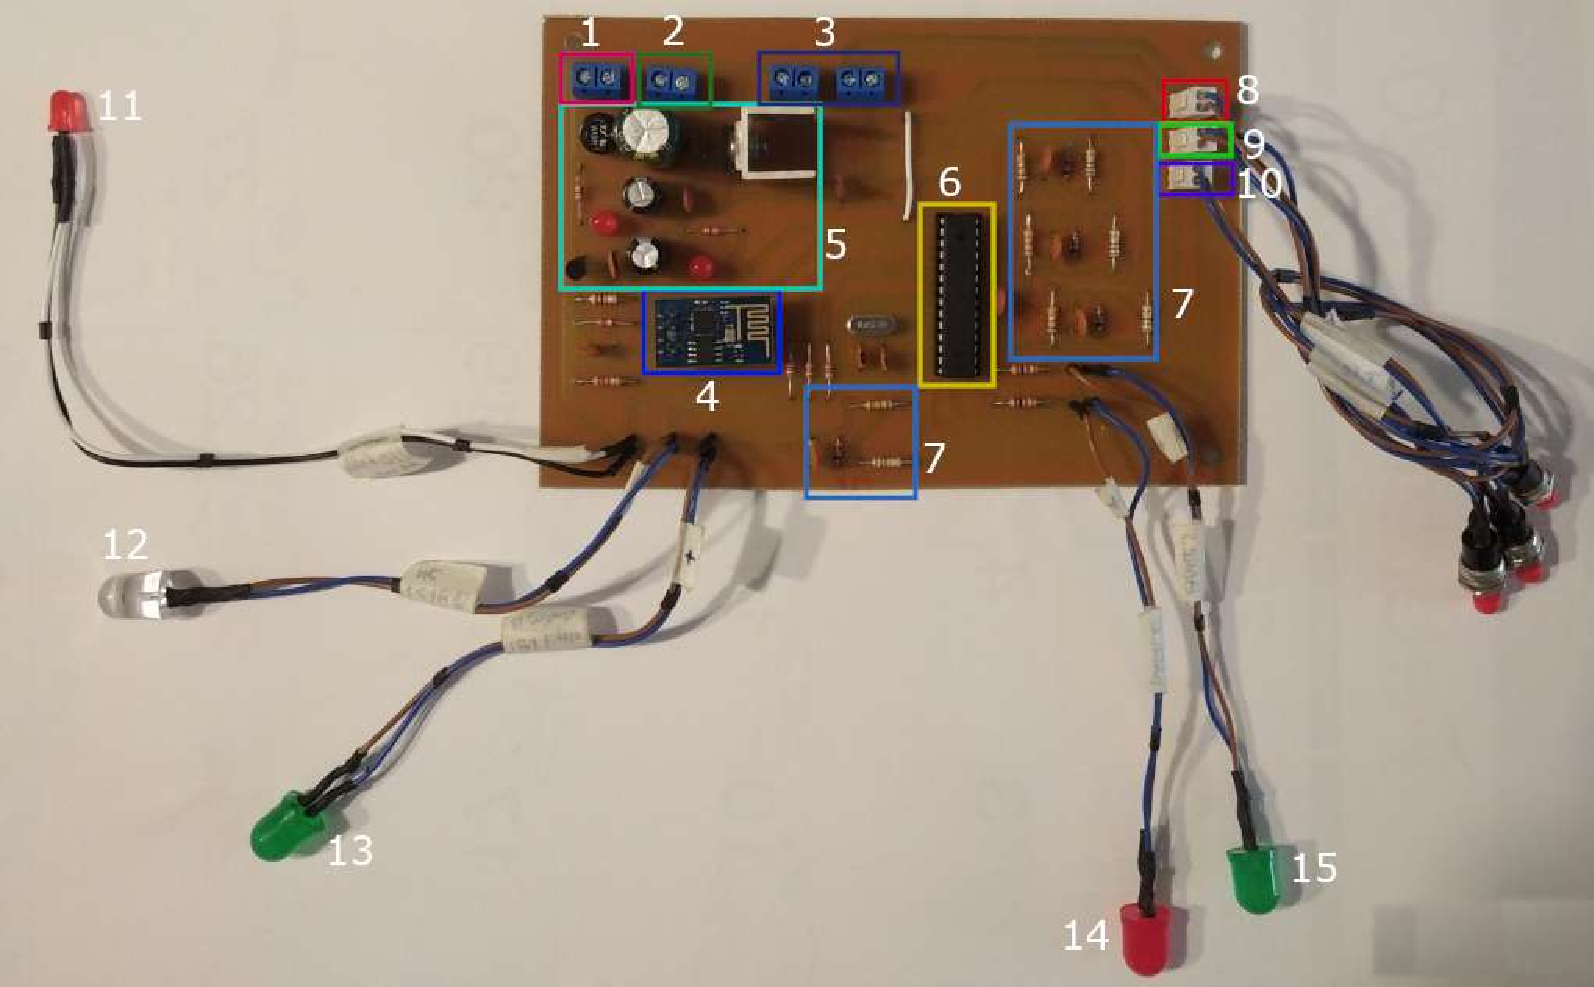
\includegraphics[width=\textwidth]{pcb_imagen_tesis.pdf}
	\caption{PCB generado a partir del diseño final.}
	\label{fig:img_pcb_imagen_tesis}
\end{figure}

Sobre la misma se ha indicado con recuadros de diversos colores las diferentes partes que la componen. Estas se detallan a continuación:

\begin{enumerate}
	\item Entrada de 12V de alterna, proveniente desde el bobinado secundario del transformador.
	\item Salida de 12V de continua destinada a la alimentación de los periféricos: las tres barreras infrarrojas y el detector magnético.
	\item Entradas provenientes desde los periféricos. Observando desde la izquierda se tiene: barrera infrarroja 3, barrera infrarroja 2, detector magnético y barrera infrarroja 1.
	\item Módulo de comunicación WiFi.
	\item Fuente regulada de tensión continua.
	\item Microcontrolador ATmega328P
	\item Adaptaciones de nivel de tensión entre los periféricos y los pines del microcontrolador.
	\item Pulsador de reset del microcontrolador.
	\item Pulsador para simulación del detector magnético de salida.
	\item Pulsador para simulación del retiro del ticket a la entrada.
	\item Led indicador de falla del Módulo WiFi.
	\item Led indicador de falla del Microcontrolador.
	\item Led para simulación de impresión del ticket.
	\item Led para simulación de barrera de entrada.
	\item Led para simulación de barrera de salida.
\end{enumerate}




\section{Periféricos}
En la presente sección, se realiza una breve descripción de los periféricos que forman parte del sistema, que fueron proporcionados por la empresa interesada en el desarrollo de este proyecto.

\subsection{Barreras Infrarrojas}

El sistema posee tres barreras infrarrojas que componen el sistema de detección de tamaño de los vehículos que desean ingresar a los establecimientos. Uno de esos equipos se observa en la figura~\ref{fig:img_Barrera_infrarroja}.

\begin{figure}[H]
	\centering
	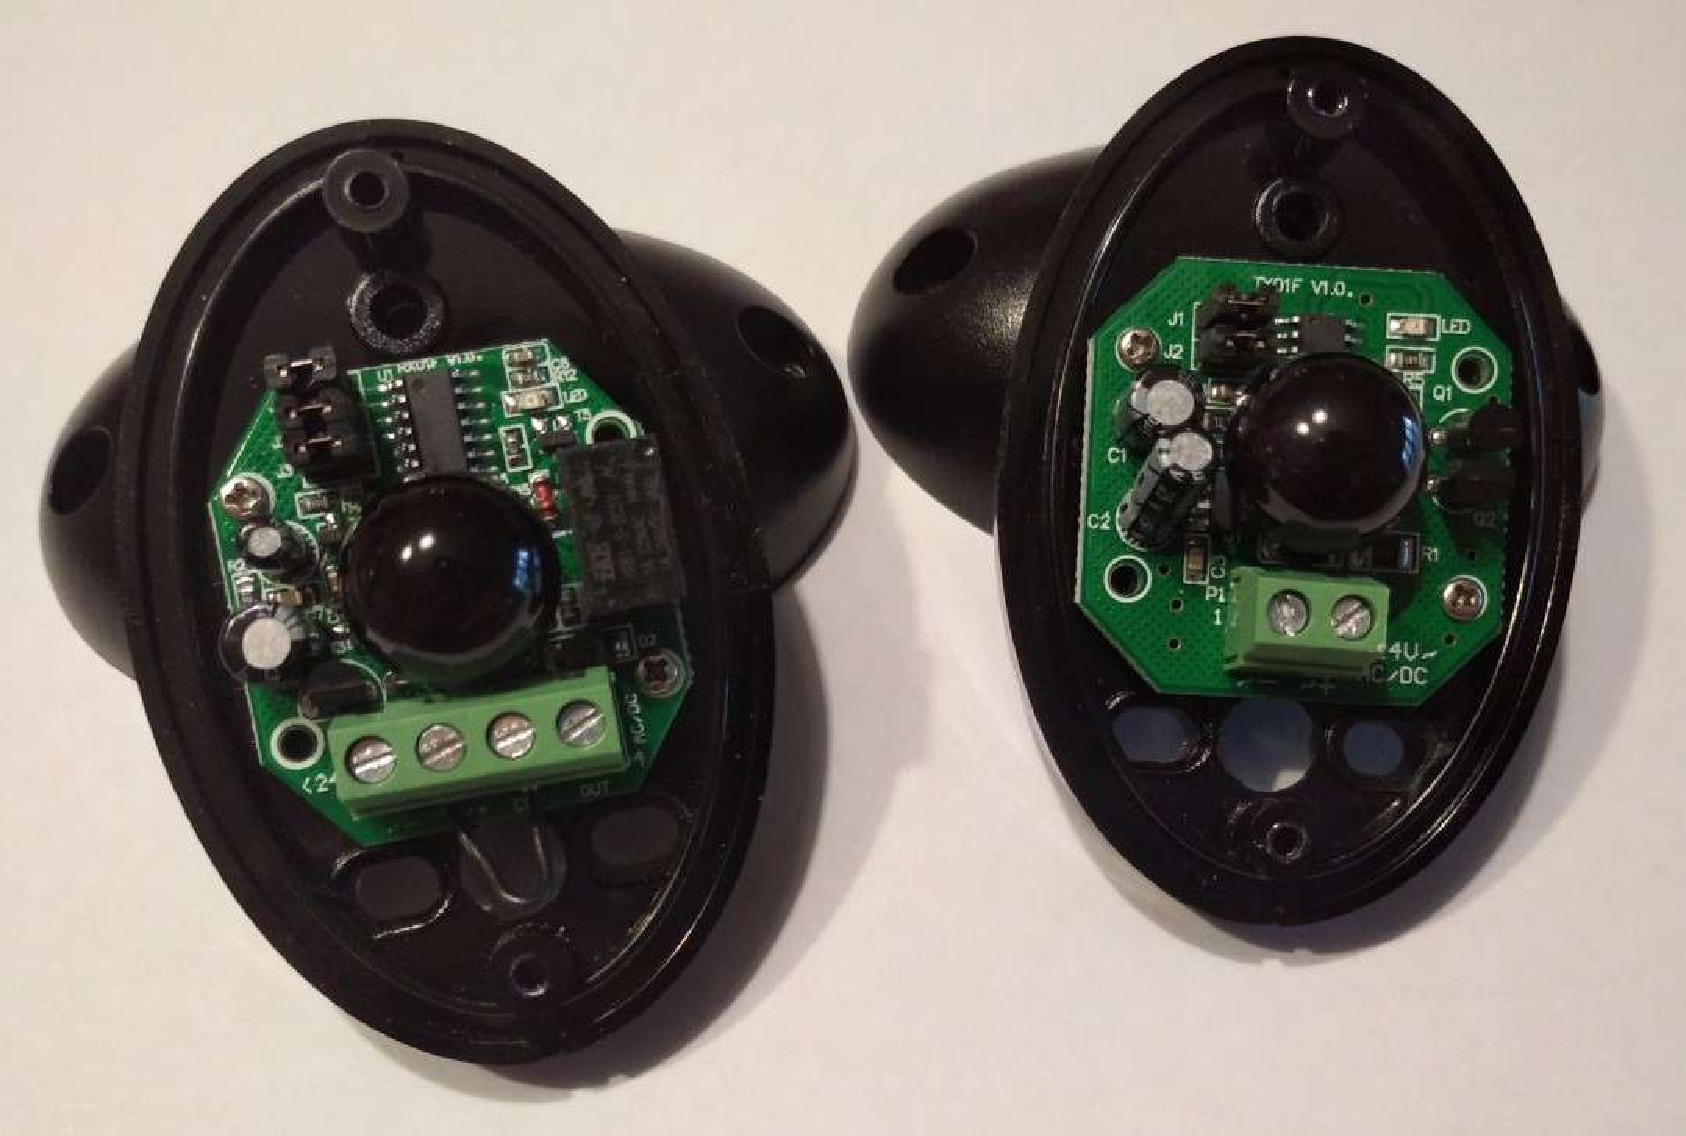
\includegraphics[scale=0.3]{Barrera_infrarroja.pdf}
	\caption{Barrera infrarroja utilizada: receptor (izquierda) y transmisor (derecha).}
	\label{fig:img_Barrera_infrarroja}
\end{figure}

Las características más relevantes de este modelo de barrera son las siguientes:
\begin{itemize}
	\item Alcance $\leq$ 15m
	\item Tensión de operación: DC/AC 12-24V
	\item Consumo de corriente del receptor: 15mA
	\item Consumo de corriente del transmisor: 30mA
\end{itemize}

Por otra parte, tanto el equipo transmisor como el receptor poseen dos jumpers J2 y J3. Estos se utilizan para determinar la frecuencia de trabajo de la barrera. A partir de los mismos, existen cuatro combinaciones correspondientes a cuatro frecuencias distintas. Esto permite que barreras cercanas trabajen a diferentes frecuencias y se evita que se produzcan interferencias entre ellas.

Adicionalmente, el receptor posee un jumper adicional J1 que se utiliza para determinar si el contacto disponible de su relé interno es el normal cerrado o el normal abierto.

En la figura~\ref{fig:img_Barrera_infrarroja}, se observa el diagrama de conexiones del receptor (izquierda) y del transmisor (derecha). Mientras el segundo únicamente requiere tensión de alimentación, el primero también posee el común y la salida del relé interno. En el sistema, el común se encuentra conectado a la tensión de alimentación para que, en caso de activarse la barrera, a la salida del relé se tengan los 12V de entrada. Estos 12V son acondicionados mediante la adaptación de niveles para que al microcontrolador lleguen 5V. 

\begin{figure}[H]
	\centering
	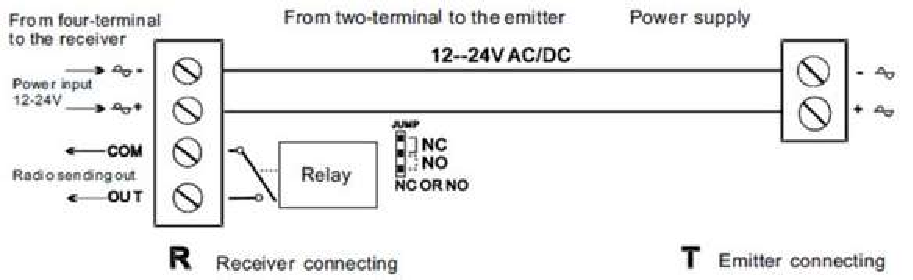
\includegraphics[width=\textwidth]{Conexion_barreras_infrarrojas.pdf}
	\caption{Conexiones de la barrera infrarroja: receptor (izquierda) y transmisor (derecha).}
	\label{fig:img_Conexion_barreras_infrarrojas}
\end{figure}

Finalmente, en lo que respecta al aseguramiento del correcto funcionamiento de este equipo, el mismo debe ser colocado al menos a 20cm de altura y con una distancia mayor a 1m entre receptor y transmisor.


\subsection{Detector de presencia magnético}

El sistema posee dos detectores de presencia magnéticos, aunque uno de ellos se encuentra simulado. Mientras que uno de ellos se ubica en el ingreso al establecimiento, el otro se encuentra en el egreso del mismo. Se lo puede observar en la figura~\ref{fig:img_Det_Mag}.

\begin{figure}[H]
	\centering
	\includegraphics[scale=0.6]{Det_Mag.pdf}
	\caption{Detector magnético utilizado.}
	\label{fig:img_Det_Mag}
\end{figure}

Respecto al funcionamiento, al momento de darle alimentación, el detector se sintoniza automáticamente con el lazo inductivo que tiene conectado. El equipo requiere una tensión de alimentación de 12V DC/AC y \textcolor{mGreen}{tiene un consumo de corriente de X (verificarlo al probarlo)}.

Por otra parte, el equipo posee dos indicadores leds que se encenderán según el estado en el que el mismo se encuentra. Cuando está sintonizado, se encienden el led rojo (power) y el verde (detect). Luego de dos segundos, el verde se apaga. Por su parte, mientras el equipo se encuentre alimentado, el led rojo se encuentra siempre encendido. El verde, va a parpadear en caso de falla o va a quedar encendido cuando se detecte un vehículo atravesando el lazo.

El diagrama de conexiones se muestra en la figura ~\ref{fig:img_Conexiones_det_mag}. Los pines 1 y 2 están destinados a la alimentación del detector. Los pines 5, 6 y 10 forman parte del relé de presencia del sistema. Entre 5 y 6 se tiene el contacto normal abierto y entre 6 y 10 el normal cerrado. Los pines 3, 4 y 11 forman parte del relé de salida pulsada. Entre 3 y 4 se tiene el contacto normal abierto y entre 4 y 11 el normal cerrado. Al momento de detectar la presencia de un vehículo, puede utilizarse tanto la salida del relé de presencia como el de pulso. Mientras que el primero es energizado mientras el vehículo se encuentra sobre el lazo, el segundo lo hace cuando el vehículo ingresa al lazo o cuando sale de él. Esto último es configurable. Finalmente, entre los pines 7 y 8 se conecta el lazo inductivo.

\begin{figure}[H]
	\centering
	\includegraphics[scale=0.6]{Conexiones_det_mag.pdf}
	\caption{Conexiones de la barrera infrarroja: receptor (izquierda) y transmisor (derecha).}
	\label{fig:img_Conexiones_det_mag}
\end{figure}

Como se observa en la figura~\ref{fig:img_Det_Mag}, en el frente del detector hay 8 selectores que permiten configurar el equipo:
\begin{itemize}
	\item \textbf{Ajuste de frecuencia:} corresponde a los primeros dos selectores. Hay cuatro combinaciones o frecuencias posibles. Esto permite que detectores que están ubicados cerca operen a diferentes frecuencias y no interfieran entre sí.
	\item \textbf{Ajuste de sensibilidad:} corresponde a los siguientes tres selectores (3, 4 y 5). Hay ocho posibilidades, que hacen que el sensor sea más o menos selectivo al momento de realizar la detección.
	\item \textbf{Filtro:} permite eliminar las interferencias del entorno. Se lo activa seteando en ON el selector 6. Cuando se encuentra activado, el tiempo de reacción del detector aumenta y la sensibilidad se ve reducida. Es por esto que, a menos que el entorno lo requiera, no debe activarse.
	\item \textbf{Salida de relé:} corresponde al selector 7. Solo afecta a la salida del relé de pulso. Si se lo setea en OFF, el relé se energiza cuando un vehículo ingresa al lazo. En caso contrario, el mismo es energizado cuando el vehículo egresa del lazo. 
	\item \textbf{Tiempo de presencia:} corresponde al selector 8. Permite determinar si el relé de presencia mantiene la presencia detectada hasta que el vehículo deja el lazo o si lo hace solo por diez minutos.
\end{itemize}

En caso de hacer alguna modificación en la configuración es necesario volver a sintonizar el detector. Para ello, puede utilizarse el botón de reset.

Respecto al lazo inductivo, el mismo debe realizarse con cable de $1.5mm^{2}$ de área y debe tener forma rectangular. La cantidad de vueltas que posee depende de las dimensiones con las que se lo construya. Basándose en el manual de usuario y en el tamaño de las vías de acceso de los establecimientos relevados, en este proyecto se consideró el uso de un lazo de 2.5m de largo por 1m de ancho, al que le corresponden cuatro vueltas de cable. Adicionalmente, los extremos del cable del lazo debe trenzarse, con al menos veinte vueltas por metro. Esto último tiene por objetivo que el cable de conexión del lazo no forme parte del área de detección, evitando que participe de la misma.

En caso de que el detector no funcione correctamente, se debe proceder de la siguiente manera:
\begin{itemize}
	\item Verificar el estado del lazo inductivo y del cableado
	\item Modificar la sensibilidad y/o la frecuencia
	\item Setear el filtro en ON
\end{itemize}










%\chapter{Prototipo desarrollado} \chapterlabel{Primer_prototipo} \label{cap:prototipo1v2}

\section{Introducción}\label{sec:introProto1}

Como se mencionó previamente, el proyecto se llevó a cabo en forma incremental. Esta modalidad consiste en desarrollar núcleos pequeños que, una vez completados, evolucionan mediante el agregado de nuevas funcionalidades y el mejoramiento de aquellas que ya poseían.

Se realizaron dos prototipos. El primero de ellos se enfocó en lograr la lectura de la patente, la detección de la presencia del vehículo y la manipulación de una barrera, considerando una sola vía de acceso.

Una vez que este primer módulo se puso a punto, se mejoraron algunas de sus funcionalidades y se le añadieron nuevas, dando lugar al segundo prototipo. 


\section{Prototipo inicial}

En la etapa inicial del proyecto se desarrolló un primer prototipo cuyo objetivo principal fue lograr la correcta obtención las patentes de los vehículos detectados. Por este motivo, en esta fase no se tuvieron en cuenta varios aspectos que se presentan en un escenario real, como por ejemplo, la diferenciación entre vía de ingreso y de egreso.

Durante la realización de este prototipo se desarrollaron tres códigos en lenguaje C++, uno para la UCC, otro para el módulo WiFi y un tercero para la Placa I/O. El primero de ellos fue diseñado en el entorno de desarrollo Eclipse \cite{eclipse}, el cual es una plataforma de software compuesto por un conjunto de herramientas de programación de código abierto y multiplataforma. Por otra parte, los otros dos códigos fueron desarrollados mediante el IDE (Integrated Development Environment) de Arduino \cite{arduinoide}, debido a que tanto el microcontrolador como el módulo WiFi utilizados son compatibles con el software que provee esta compañía.

A continuación, se detalla el funcionamiento de este primer prototipo.
En primer lugar, se lleva a cabo una etapa de conexión entre el módulo WiFi, la Placa I/O y la UCC. En esta, al encender el sistema, la Placa I/O pone en alto el pin de reset del módulo WiFi produciendo el arranque del mismo.

Una vez encendido, el módulo procede a conectarse a la red WiFi local creada mediante un router y, luego, genera un servidor web en su dirección IP. A partir de este momento, la placa y el módulo quedan a la espera de que la UCC se conecte a dicho servidor. La primera acción que esta última lleva a cabo es la creación un socket TCP/IP, el cual utiliza para conectarse al servidor mencionado anteriormente. De esta manera, se concluye la etapa de conexión y el sistema queda listo para funcionar en modo continuo.

Cuando se presiona alguno de los dos pulsadores, acción que representa la detección de un vehículo mediante uno de los sensores magnéticos, el microcontrolador de la Placa I/O recibe dicha información y se la envía por puerto serie al módulo WiFi. Este último, comunica la información sobre el estado de los magnéticos a la UCC vía WiFi, únicamente si alguno de ellos fue activado. 

Entonces, cuando a la UCC le llega esta información, a partir del procesamiento de los trabajos generados por el OpenALPR, se obtiene la patente del vehículo detectado.

En esta etapa, la activación de cualquiera de los pulsadores por separado, o de ambos simultáneamente, desemboca en la misma condición: la activación del sistema de reconocimiento de patentes sin discriminación entre entrada o salida. Esto se debe a que aún no se desarrolló esta distinción, ya que el principal objetivo de este primer prototipo es la verificación del correcto funcionamiento del reconocimiento. Luego de que se obtuvo la patente, la Unidad Central se la envía a la Placa I/O, de manera de indicarle que levante la barrera.

Cabe destacar que los tres códigos fueron desarrollados de manera secuencial. Esto implica que, si por ejemplo se activa algún detector magnético mientras se lleva a cabo un proceso de ingreso o egreso anterior, el sistema no podrá responder a dicho evento.



\section{Prototipo final}

En esta sección, se desarrollará el funcionamiento del prototipo final del proyecto. En este, la principal modificación fue la coexistencia de dos vías, una de ingreso y otra de egreso, funcionando simultáneamente. Para realizar esto se utilizó el software YAKINDU Statecharts Tools \cite{yakinduprincipalpage} con una licencia académica, la cual brinda acceso a todas sus funcionalidades seis meses. Además, su entorno de desarrollo está basado en Eclipse, lo que facilitó su uso, ya que dicho software fue implementado al realizar el prototipo inicial.

Este framework es capaz de generar bloques de código en diferentes lenguajes tales como C, C++ o Java, a partir de una máquina de estado conformada mediante diagramas UML (Unified Modeling Language). En la figura~\ref{fig:img_statemachintable} se presenta una tabla comparativa entre las máquinas de estado UML y otros tipos, donde se observan las ventajas que las primeras poseen sobre las demás.

\begin{figure}[H]
	\centering
	\includegraphics[width=\textwidth]{statemachintable.pdf}
	\caption{Comparación entre diferentes máquinas de estado \cite{yakindustatemachine}.}
	\label{fig:img_statemachintable}
\end{figure}

Los sistemas diseñados a partir de esta herramienta tienen dos formas de funcionamiento: basadas en ciclos o basadas en eventos \cite{yakinduevent-cycle}. Para cualquiera de los dos casos, un ciclo es el procedimiento mediante el cual el sistema analiza si debe pasar o no al siguiente estado, en cada una de las regiones que posea. La diferencia entre éstas dos formas de funcionamiento radica en el disparador del siguiente ciclo. En el primer caso, el sistema ejecuta su siguiente ciclo cada un cierto periodo de tiempo fijo, mientras que en la segunda forma, se espera a que algún evento haya ocurrido para ejecutar el ciclo. Debido a que en este proyecto se requiere que determinadas acciones sucedan a lo largo del ingreso o egreso para poder avanzar, se ha diseñado un sistema basado en eventos.

Por otra parte, mediante esta herramienta es posible generar sistemas basados en la técnica de la multiprogramación, es decir, la ejecución de tareas de manera concurrente por el procesador a tal velocidad que causa la impresión de ser en paralelo. Esto es de vital importancia para poder considerar a la entrada y la salida como dos vías independientes, permitiendo efectuar ambos procesos simultáneamente. Además, al igual que el entorno de Eclipse, este software permite el desarrollo de proyectos de Arduino, que pueden ser cargados sobre las placas de dicha compañía. Debido a estas razones, tanto el código de la UCC como el de la Placa I/O fueron desarrollados mediante esta herramienta. Cabe destacar que el código correspondiente al módulo WiFi se generó con el IDE de Arduino, ya que no presentó gran complejidad debido a que únicamente es un intermediario entre la UCC y la placa. En la figura~\ref{fig:img_diagrama-comunicacion} se puede observar un diagrama en bloques representativo de la comunicación dentro del sistema.

\begin{figure}[H]
	\centering
	\includegraphics[width=\textwidth]{diagrama-comunicacion.pdf}
	\caption{Comunicación entre UCC, Módulo y Placa.}
	\label{fig:img_diagrama-comunicacion}
\end{figure}

En las siguientes secciones de este capítulo se desarrollará el funcionamiento de cada una de las etapas del sistema.  Se destaca que, a pesar de que su funcionamiento se explique en forma individual, las mismas trabajan en forma conjunta, a excepción de la fase de conexión.
  

\subsection{Fase de conexión}

En esta primera etapa, se busca establecer la conexión entre la UCC, el módulo WiFi y la Placa I/O. Esta fase ocurre solamente al iniciaro el sistema.

Cada uno de los códigos desarrollados con el software YAKINDU posee una región específica para esta etapa, y las mismas se pueden observar en las figuras \ref{fig:img_ConexionPlaca} y \ref{fig:img_ConexionUCC}. Por otra parte, en el módulo WiFi, esto sucede dentro del setup de Arduino, como se ve en la figura~\ref{fig:img_setupmodwifi}. 

\begin{figure}[H]
	\centering
	\begin{subfigure}[b]{0.49\textwidth}
		\includegraphics[width=\textwidth]{ConexionPlaca.pdf}
		\caption{Región de conexión de Placa I/O.}
		\label{fig:img_ConexionPlaca}
	\end{subfigure}
	\hfill
	\begin{subfigure}[b]{0.49\textwidth}
		\includegraphics[width=\textwidth]{ConexionUCC.pdf}
		\caption{Región de conexión de UCC.}
		\label{fig:img_ConexionUCC}
	\end{subfigure}
	\hfill
	\begin{subfigure}[b]{0.49\textwidth}
		\includegraphics[scale=0.7]{setupmodwifi.pdf}
		\caption{Conexión del módulo WiFi.}
		\label{fig:img_setupmodwifi}
	\end{subfigure}
	\caption{Proceso de establecimiento de la conexión entre UCC, módulo WiFi y Placa I/O.}
\end{figure}

Al encender la Placa I/O, el microcontrolador pone en alto uno de sus pines digitales, el cual se encuentra conectado al pin de reset del módulo WiFi. De esta manera, el funcionamiento de este último queda controlado por la placa. Debido a que al iniciar el módulo el mismo escribe caracteres residuales en su puerto serie, la placa tiene un tiempo de espera de 15 segundos antes de inicializar dicha comunicación. De esta manera, se evita que estos caracteres afecten el funcionamiento normal de la placa. Luego de este período, esta última permanece a la espera de que se establezca la conexión por parte de la UCC.

Como se observa en la figura~\ref{fig:img_setupmodwifi}, luego de iniciar, el módulo WiFi se conecta a la red WiFi que se le indica, crea un servidor web y queda a la espera de que la UCC se conecte al mismo. En caso de no poder conectarse a la red correspondiente, el módulo encenderá un led que indica la existencia de una falla.

Por su parte, la UCC debe conectarse al servidor creado. Para esto, luego de inicializar las variables necesarias, procede a crear un socket TCP/IP y conectarse a través de este al servidor. Es preciso mencionar que, en caso de falla en la creación o en la conexión del socket, el sistema informa dichos errores en pantalla.

Una vez establecida la conexión, la UCC le envía un mensaje al módulo WiFi indicándole este suceso, terminando su parte en la etapa de conexión. Al recibirlo, el módulo lo reenvía a la placa, poniendo fin a la etapa de conexión en su totalidad. De esta manera, el sistema queda preparado para su funcionamiento en forma continua. Se debe tener en cuenta que si se inicializa el código de la UCC en simultáneo con la placa, este mensaje que se envía se pierde. Esto se debe a los 15 segundos de demora establecidos en el microcontrolador para iniciar la comunicación serie. Por tal motivo, luego de este tiempo, la placa enciende durante dos segundos su led de falla, indicando que está preparada para la recepción de mensajes. Entonces, el código de la UCC debe ejecutarse luego de la ocurrencia de este evento.


\subsection{Envío y recepción de mensajes}

En los tres sistemas, al recibir un mensaje, este es contestado por el receptor con un mensaje de ACK para confirmar su llegada. Debe aclararse que los mensajes de ACK recibidos no se contestan. Por otra parte, al enviar un mensaje diferente de ACK, todos los sistemas deben recibir su respectivo mensaje de confirmación. De esta manera, se puede comprobar el arribo de todos los mensajes que se envían de un punto a otro. En caso de que un mensaje de ACK no se reciba en el plazo de 10 segundos establecido, se enciende un led de falla o se muestra un mensaje de error en pantalla, dependiendo de qué sistema no lo recibió. Ante una falla de este tipo, se determinó que el sistema deje de funcionar. A futuro, se implementará una solución que no implique reiniciar el sistema manualmente.

El envío y recepción de mensajes es la función principal del módulo WiFi, ya que se encarga de tomar los mensajes provenientes de un extremo y enviarlos al otro. Por lo tanto, el módulo no es más que un intermediario entre la placa y la UCC.

Por su parte, la Unidad Central posee una región especial que se encarga de comprobar si todos los ACK fueron recibidos correctamente.  La misma se activa cada vez que en alguna parte del código se ejecuta la función de envío de mensajes. Esto puede observarse en la figura~\ref{fig:img_WaitACKUCC}.

\begin{figure}[H]
	\centering
	\includegraphics[width=\textwidth]{WaitACKUCC.pdf}
	\caption{Control de ACK de la UCC.}
	\label{fig:img_WaitACKUCC}
\end{figure}

En cuanto a la recepción de mensajes, la UCC se encuentra continuamente verificando si llegó alguno nuevo. En caso de que esto ocurra, informa en pantalla lo que recibió y procede a ejecutar las acciones que correspondan, ya sea modificar algún valor, levantar algún evento, entre otras.

Por otra parte, la Placa I/O posee dos regiones, una destinada a la recepción de mensajes y otra para el envío de los mismos. Estas pueden observarse en las figuras~\ref{fig:img_RcvMSGPlaca} y \ref{fig:img_SendMSGPlaca}, respectivamente.

\begin{figure}[H]
	\centering
	\includegraphics[width=\textwidth]{RcvMSGPlaca.pdf}
	\caption{Recepción de mensajes desde Placa I/O.}
	\label{fig:img_RcvMSGPlaca}
\end{figure}

\begin{figure}[H]
	\centering
	\includegraphics[width=\textwidth]{SendMSGPlaca.pdf}
	\caption{Envío de mensajes desde Placa I/O.}
	\label{fig:img_SendMSGPlaca}
\end{figure}

En la figura~\ref{fig:img_RcvMSGPlaca}, se pueden observar las diferentes reacciones del sistema ante la recepción de un ACK, de la información del vehículo o cualquiera de los otros posibles mensajes. Por otra parte, en la región de envío de mensajes, se puede visualizar el estado WaitACK, donde el sistema comprueba el arribo de ACKs para los mensajes que haya enviado.


\subsection{Vía de ingreso}

Tanto la UCC como la Placa I/O disponen de una región destinada al funcionamiento de la vía de ingreso al establecimiento.  Éstas dos se pueden observar en las figuras~\ref{fig:img_EntradaUCC} y~\ref{fig:img_EntradaPlaca}, respectivamente. Por su parte, durante esta etapa, el módulo WiFi solo envía los mensajes que recibe, de un extremo al otro.

\begin{figure}[H]
	\centering
	\includegraphics[width=\textwidth]{EntradaUCC.pdf}
	\caption{Procedimiento sobre la Vía de ingreso de la UCC.}
	\label{fig:img_EntradaUCC}
\end{figure}

\begin{figure}[H]
	\centering
	\includegraphics[width=\textwidth]{EntradaPlaca.pdf}
	\caption{Procedimiento sobre la Vía de ingreso de la Placa I/O.}
	\label{fig:img_EntradaPlaca}
\end{figure}


En la vía de ingreso, la placa se encuentra verificando continuamente el estado del detector magnético. Una vez que este se activa, comienza el funcionamiento de la región mostrada en la figura~\ref{fig:img_EntradaPlaca}. La primera acción de la misma es comunicarle a la UCC que un nuevo vehículo ha ingresado al estacionamiento. Al recibir esta información, la UCC levanta el evento ``NewEntry'' y procede con la fase de obtención de la patente.

Para obtener la matrícula, en primera instancia , la UCC inserta un trabajo bandera del cual se guarda el número de ID. Este se utiliza como guía para eliminar todos los trabajos anteriores acumulados en la cola, que poseen un número de ID inferior al mismo, evitando así que se efectúe una lectura errónea. Una vez que estos son eliminados, se procede a analizar los nuevos trabajos que el sistema va agregando a la cola hasta alcanzar una cifra de nueve, o bien, hasta que transcurran dos segundos. Luego, dado que se obtiene un resultado para la patente por cada trabajo analizado, la respuesta a devolver corresponderá a aquel que más veces se presente. Cabe destacar que, de esta manera, el sistema puede obtener diferentes posibles resultados para la misma patente. Por lo tanto, en caso de que se produzca un empate entre la cantidad de ocurrencias de dos (o más) resultados, se elige aquel que presente un valor de confianza mayor. Por otra parte, en caso de que no se logre analizar ningún trabajo, el sistema entrega como respuesta un número de siete cifras que representa un patente provisoria.

Con el resultado de la patente obtenido, la UCC debe verificar si el vehículo que desea ingresar al establecimiento es un cliente nuevo o un abonado. Para realizar esto se implementó una base de datos sencilla basada en MySQL. Este es un sistema de gestión de bases de datos desarrollado en C/C++ bajo licencia dual: Licencia pública general/Licencia comercial, por Oracle Corporation, y está considerada como la base de datos de código abierto más popular del mundo \cite{mysql}.

La base de datos creada consta de tres tablas independientes. En la primera de ellas, denominada ``Regular'', se registran todos los vehículos abonados, es decir, aquellos que pagan una tarifa mensual. En la segunda, llamada ``Parking'', se almacenan todos los automóviles que hayan ingresado al establecimiento y aún no se hayan retirado. Esto implica que, con esta tabla, se puede saber la cantidad de vehículos estacionados dentro del estacionamiento. Por último, la tabla denominada ``History'', lleva un historial de todos los vehículos que han ingresado y salido del establecimiento.

Entonces, para determinar si un vehículo es abonado o no, la UCC verifica si su patente se encuentra en la tabla ``Regular''. La misma se observa en la figura~\ref{fig:img_BDREGULAR}. Luego, se ingresa la información de la patente, la fecha y hora de ingreso a la tabla ``Parking'', la cual se ve en la \hl{figura x10 (poner antes de que se actualice el tipo)}. Por último, se informa a la placa de qué tipo de cliente se trata. En el caso de un abonado, además de la información mencionada, también se añade el tipo de vehículo y el estado del pago a dicha tabla.

\begin{figure}[H]
	\centering
	\includegraphics[scale=1]{BDREGULAR.pdf}
	\caption{Tabla ``Regular'' de la base de datos desarrollada.}
	\label{fig:img_BDREGULAR}
\end{figure}

%\begin{figure}[H]
%	\centering
%	\includegraphics[width=\textwidth]{figura x10.pdf}
%	\caption{Tabla “Parking” de Base de Datos(poner q se ve un abonado y un no abonado).}
%	\label{fig:img_}
%\end{figure}

Mientras la placa espera que la UCC envíe la información acerca de la clase de cliente, calcula el tipo de vehículo que intenta ingresar: auto, moto o camioneta. Para ello, se implementa un sistema constituido por tres barreras infrarrojas, las cuales se encuentran dispuestas cada 2.5m. Se determinó que esta debía ser la distancia, a raíz de una investigación realizada sobre el tamaño máximo y mínimo que pueden tener los tres tipos de vehículos a detectar. En cuanto a su funcionamiento, el sistema analiza cuántas de las tres barreras son cortadas simultaneamente por el vehículo que ingresa, cuando la más cercana de ellas a la barrera es activada. En caso de que los tres haces infrarrojos sean interrumpidos, se trata de una camioneta. Por otra parte, si solo los 2 sensores más próximos a la barrera se encuentran activados, es un auto. Finalmente, si no se activa más de una barrera a la vez, el vehículo es una motocicleta. De esta forma, se determina la tarifa que debe abonarse, ya que en muchos estacionamientos del país se cobra un monto diferenciado según el tipo de automóvil.

En el caso de un cliente abonado, luego de enviar la información mencionada anteriormente, la UCC vuelve a quedar a la espera de un nuevo ingreso. Por otra parte, la placa al recibir esta información, descarta el cálculo del tipo y el retiro del ticket, y le permite el ingreso al estacionamiento levantando la barrera. Esto se puede visualizar con el encendido de un led, durante dos segundos, que representa la barrera.

En el caso de un cliente no abonado, luego de informar su clase, la UCC espera recibir el tipo de vehículo para actualizar la tabla de la base de datos. Esto se observa en la \hl{figura x11}. 

%\begin{figure}[H]
%	\centering
%	\includegraphics[width=\textwidth]{figura x11.pdf}
%	\caption{Tabla "parking" con tipo de vehículo actualizado.}
%	\label{fig:img_}
%\end{figure}

Al recibir que se trata de un no abonado, la placa le informa a la UCC el ``tipo'' que determinó, y queda a la espera de la patente y la hora de ingreso. Estos datos se presentarían en el ticket que se le entrega a los usuarios, pero, en este caso, la impresión del mismo se encuentra simulada por el encendido de un led. Por lo tanto, al recibir la información del tipo, la UCC responde con estos datos, terminando su participación en el proceso de entrada. Al recibir dicha información, la placa enciende el led que indica que el ticket fue impreso. 

Por último, para permitir el acceso al establecimiento, el usuario debe retirar el ticket. En este caso, esta acción se encuentra representada por la activación de un pulsador. Entonces, al presionarlo, se lleva a cabo el retiro del ticket, se apaga el led de ticket impreso y se enciende, durante dos segundos, el led que simula la barrera. De esta manera, se concluye el ingreso del vehículo.

Debe tenerse en cuenta que, si se activa el detector magnético mientras está ingresando otro vehículo, esta condición se guarda. Por lo tanto, luego de que se apague el led de barrera, la placa no vuelve a su estado de espera, sino que comienza directamente con el proceso de ingreso pendiente.

Finalmente, en el caso de vehículos que no posean patentes, o que la misma no se haya podido obtener, el sistema igualmente permite el ingreso y se establece una patente provisoria, como se mencionó anteriormente.


\subsection{Vía de egreso}

De manera similar al caso de la vía de ingreso, tanto la Placa I/O como la UCC tienen una región destinada a la salida del vehículo, mientras que el módulo WiFi solo retransmite los mensajes. Ambas regiones pueden visualizarse en las figuras~\ref{fig:img_SalidaPlaca} y~\ref{fig:img_SalidaUCC}, respectivamente.

\begin{figure}[H]
	\centering
	\includegraphics[width=\textwidth]{SalidaPlaca.pdf}
	\caption{Etapa de egreso de la Placa I/O.}
	\label{fig:img_SalidaPlaca}
\end{figure}

\begin{figure}[H]
	\centering
	\includegraphics[width=\textwidth]{SalidaUCC.pdf}
	\caption{Etapa de egreso de la UCC.}
	\label{fig:img_SalidaUCC}
\end{figure}

Al igual que en la vía de ingreso, el sistema se encuentra a la espera de la activación del detector magnético. Cuando la Placa I/O verifica que un nuevo vehículo desea retirarse del establecimiento, lo informa a la UCC y se mantiene a la espera de la respuesta de ésta.

La única diferencia con la entrada es que en caso de no detectar ninguna patente, se establece el valor ``NoPlate'' como resultado. 

Al recibir esta información, el proceso seguido por la UCC para obtener la patente del vehículo que activó el sistema es idéntico al de la entrada. La UCC debe verificar que la matrícula detectada se encuentre en la tabla ``Parking'', es decir, que se comprueba que el vehículo haya ingresado. Por lo tanto, en este punto tenemos dos posibilidades:

\begin{enumerate}
	\item \textbf{La patente se encuentra en la base de datos.} En este caso, se verifica si el cliente ya realizó el pago de la tarifa. Con la finalidad de ensayar el prototipo, se diseñó un código que lo simula. En este, se le pide al operario que ingrese la patente, la tarifa y si el pago fue efectuado. De esta manera, se actualiza la información de la tarifa, el estado del pago y la fecha y hora de salida en la tabla “Parking”, de la base de datos. En la \hl{figura x11}, se puede observar que dichos campos se encontraban vacíos, mientras que en la \hl{figura x14} se ve que fueron actualizados. Por lo tanto, la UCC avisa a la placa que el egreso es permitido o denegado dependiendo de esta condición.
	
	\item \textbf{La patente no se encuentra en la base de datos.} En este caso, se informa por pantalla al operario de lo sucedido, y este debe verificar si fue un error en la detección de la patente o no, visualizando el vehículo. En el primer caso, se le pide que ingrese la patente correcta y el sistema la vuelve a buscar en la base de datos, llevando a cualquiera de éstas posibilidades nuevamente. Se destaca que, en el caso de no poder detectar correctamente la patente, si a la entrada se asignó una provisoria, se debe ingresar ese valor. En el segundo caso, se avisa a la placa que el egreso fue denegado.
	\end{enumerate}

%\begin{figure}[H]
%	\centering
%	\includegraphics[width=\textwidth]{figura x14.pdf}
%	\caption{Tabla “Parking” con valores actualizados.}
%	\label{fig:img_}
%\end{figure}

Por lo tanto, luego de verificar en la base de datos, la UCC informa a la placa sobre si la salida es autorizada o no. Esto lleva a dos casos posibles:

\begin{enumerate}
	\item \textbf{Salida autorizada.} En este caso, la placa enciende durante dos segundos el led que simula la barrera de salida, permitiendo el egreso del vehículo. Una vez que se completa el egreso, la placa se lo informa a la UCC, terminando su parte en el proceso y quedando a la espera de un nuevo egreso. De esta manera, al recibir esta información, la UCC elimina al vehículo de la tabla “Parking” y lo agrega a la tabla “History”. Esto se puede observar en las \hl{figuras x15 y x16,} respectivamente. Luego de esta actualización, el proceso actual finaliza y la UCC queda preparada para el arribo de un nuevo vehículo.
	
	%\begin{figure}[H]
	%	\centering
	%	\includegraphics[width=\textwidth]{figura x15.pdf}
	%	\caption{Tabla “Parking” con vehículo borrado.}
	%	\label{fig:img_}
	%\end{figure}
	
	%\begin{figure}[H]
	%	\centering
	%	\includegraphics[width=\textwidth]{figura x16.pdf}
	%	\caption{Tabla “History” con vehículo agregado.}
	%	\label{fig:img_}
	%\end{figure}
	
	
	\item \textbf{Salida Denegada.} Luego de enviar esta información, la UCC se mantiene comprobando de manera continua el estado del pago de la tarifa. Esto se debe a que en el momento en que el cliente realice esta acción, se le autorizará el egreso. En caso de que la salida haya sido denegada por no encontrarse la patente en la base de datos, el sistema se queda a la espera de que el vehículo se retire de la vía de egreso, retrocediendo hacia el interior del establecimiento. Simultaneamente, la placa se encarga de analizar si el vehículo sigue posicionado sobre el detector magnético. En caso afirmativo, el cliente tiene cinco minutos para realizar el pago, si aún no lo hizo, o para retirar el vehículo de la vía de egreso. En la primera situación, al actualizarse el pago, la UCC lo verifica y se procede como en el caso de la salida autorizada. Por otra parte, si el cliente retira el vehículo de la salida, esto se informa a la UCC y el sistema finaliza el proceso, quedando preparado para recibir un nuevo vehículo.
\end{enumerate}

Cabe destacar que, en este caso, no existe la posibilidad de que un segundo vehículo active el detector magnético mientras otro realiza el ingreso. Esto se debe a que el mismo se ubica muy próximo a la barrera, por lo cual va a mantenerse activado por el mismo vehículo hasta el momento en que se retire.




%\chapter{Conclusiones y trabajos futuros} \chapterlabel{Conclusiones} \label{cap:Conclusiones}

\section{Conclusiones}

A lo largo de este documento se ha explicado la investigación, desarrollo e implementación del sistema SAE para automatizar playas de estacionamiento. Se decidió trabajar de manera incremental. Por lo tanto, se desarrolló un prototipo inicial, el cual fue progresando a medida que se avanzaba en el proyecto, debido al agregado de nuevas funcionalidades y la mejora de las ya existentes, hasta obtener un prototipo final. Mientras en el inicial se hizo hincapié en el funcionamiento de algunas etapas de gran importancia y complejidad, como es el caso de la detección de patentes, el final se enfocó en la parte de hardware. 

En el primer capítulo, se desarrolló el sistema como un producto comercial, tal como fue pensado en conjunto con la empresa que apoya este proyecto. Luego, se explicó su funcionamiento, tanto para el caso del ingreso como para el del egreso. Además, junto con los directores del trabajo final, con el objetivo de limitar el tiempo de desarrollo del proyecto y su nivel de complejidad, se estableció el alcance del mismo. De esta manera, se dejaron fuera del mismo la entrega de los tickets al ingreso y la implementación de una pantalla para  la asignación de lote, entre otras. Esto se trata con más detalle en la sección siguiente.

Por otra parte, para determinar la ubicación más adecuada de los periféricos dentro de un posible estacionamiento, se llevó a cabo un relevamiento. El mismo se abocó a las características de los establecimientos que se encuentran en la zona céntrica de la ciudad de Mar del Plata. Una posible distribución de los mismos se observa en el esquema de la figura \ref{fig:img_croquis-est}.

Debido a que el reconocimiento de las patentes es un punto crítico de este proyecto, se ha llevado a cabo una investigación exhaustiva en torno al mismo. Mediante esta, se pudieron observar los diferentes tipos de sistemas ALPR existentes, su funcionamiento general y las ventajas y desventajas que presentan. Al tratarse de una etapa crucial, se tomó la decisión de analizar dos alternativas diferentes (OpenALPR y OpenCV 3 license plate recognition), para luego optar por una de ellas. Para ambos sistemas, se llevó a cabo un análisis en detalle de su funcionamiento, se experimentó con ellos y se realizó su ajuste en base a dicha experimentación. Para ello, fue necesaria la construcción de diversos conjuntos de imágenes. A partir de los resultados obtenidos, que fueron presentados en el Capítulo \ref{cap:alpr}, se decidió continuar trabajando con el software OpenALPR. Esto se debe, principalmente, a que con esta herramienta, al reconocer la matrícula, se obtiene un porcentaje de éxito mucho mayor y en menor tiempo que con la otra alternativa.  Además, en este capítulo se muestra el relevamiento hecho sobre las características de las matrículas argentinas, considerando el modelo antiguo y el del MERCOSUR.

El otro punto crucial del sistema es el desarrollo del hardware necesario. En el Capítulo \ref{cap:2do-nucleo} se presentó el diseño y construcción de la placa encargada de controlar los equipos que se ubicarían en las zonas de ingreso y egreso. Se realizó la muestra de los esquemas circuitales correspondientes a la fuente de alimentación del sistema y la parte lógica de la placa, junto con la justificación de las diversas decisiones que se tomaron durante el diseño. Además, se realizó una breve descripción de los elementos principales del PCB, que son el microcontrolador ATmega328P y el módulo de comunicación WiFi ESP-01, y de los periféricos que integran el sistema, que son el detector vehicular magnético y las barreras infrarrojas. Finalmente, se presentó el desarrollo e implementación del circuito impreso. Para la realización del mismo, fue necesario instruirse en el uso de Altium Designer y en el método de insolado para la fabricación de placas.

El funcionamiento del sistema se basa en tres códigos diferentes, que fueron desarrollados completamente, y se encuentran distribuidos en la UCC, la Placa I/O y el Módulo WiFi. Estos fueron diseñados con el objetivo de implementar la multiprogramación. Mediante esta técnica, la ejecución de tareas por parte del procesador se da a una velocidad que causa la impresión de que ocurren en paralelo. De esta manera, se le permitió al sistema SAE poder diferenciar entre las vías de ingreso y egreso, es decir, que puede realizar el proceso de entrada y de salida en "simultáneo". Por otra parte, se añadieron al sistema funcionalidades para responder ante algunos casos particulares, como por ejemplo, un vehículo que pretende retirarse sin efectuar el pago, uno que se retire de la vía de egreso hacia el interior del establecimiento, la obtención de la matrícula de un vehículo que desea egresar y que no se encuentra en la base de datos, entre otros.

Por último, deben destacarse las características distintivas que posee el prototipo obtenido. Las mismas se enumeran a continuación:

\begin{itemize}
	\item Los sistemas de automatización investigados, tanto los implementados en los establecimientos de nuestra ciudad como los ofrecidos por empresas radicadas en la ciudad de Buenos Aires, no poseen un sistema de reconocimiento de patentes ni un sistema de detección de tamaño estandarizado.
	\item No se encontraron fabricantes de este tipo de sistemas en Mar del Plata. El desarrollo de un sistema en la ciudad permite abastecer a los establecimientos locales y proporcionarles un servicio de mantenimiento (actualmente dependen de empresas radicadas en Bs.As.).
	\item El prototipo se encuentra desarrollado completamente mediante software libre. Esto evita el pago de licencias y, en el caso del software de reconocimiento de patentes, el pago de un servicio mensual.
\end{itemize}


\section{Trabajos futuros}

El objetivo de esta sección es dejar establecidas aquellas ideas o mejoras que pueden ser implementadas en un futuro en el sistema desarrollado. Esto se debe a que, al tratarse de un proyecto de finalización de una carrera universitaria, el mismo tiene un período acotado de duración, el cual hace que muchas de estas ideas deban mantenerse fuera del mismo.

\subsection{Mejoras}
\begin{itemize}
	\item Realizar el entrenamiento del motor de OCR específico para las matrículas argentinas
	\item Desarrollo de una base de datos más compleja, que ofrezca más opciones al operador del sistema
	\item Diseño de un sistema de reseteo remoto en caso de falla en el sistema
	\item Implementación de un sistema de respaldo en caso de corte de luz
	\item Diseño y construcción de una terminal que integre la UCC, en formato All in One, junto con el lector de código de barra y la impresora de tickets fiscales
\end{itemize}

\subsection{Nuevas funcionalidades}
\begin{itemize}
	\item Agregado de impresora de tickets internos al estacionamiento, con información de hora de ingreso, número de patente y tarifa, entre otras, con su correspondiente lector de código de barra
	\item Agregado de impresora de tickets fiscales
	\item Desarrollo de una interfaz de usuario que permita el ingreso de información por parte del operario en caso de que ocurra algún inconveniente
	\item Desarrollo de un algoritmo de asignación de ubicación dentro del establecimiento y verificación del correcto estacionamiento
	\item Agregado de pantalla para mostrar el resultado de la asignación de ubicación al cliente
	\item Automatización del cobro de la tarifa a los clientes
	\item Adaptación del sistema para su aplicación en cocheras de edificios comerciales y privados, control de ingreso y egreso a barrios cerrados, etc
	\item Detección de rostros al ingreso y egreso del establecimiento, de manera de incrementar la seguridad en cuanto al retiro de los vehículos
\end{itemize}



%\chapter{COSAS QUE LUEGO DEBEN SACARSE DEL ESCRITO} \chapterlabel{Varios} \label{cap:varios}



\section{Cosas a CORREGIR del Escrito 22-02-2020}

\begin{itemize}
	\item \textbf{En cada capítulo poner al principio un resumen de lo que se va a tratar en el mismo. Poner algo similar a lo que se escribió sobre dicho capítulo al final de la Introducción general del trabajo.}
	\item Poner texto más explicativo en las figuras y las tablas. Que leyendo el epígrafe se pueda entender de qué se trata la foto. Por ejemplo, “imagen original” o “imagen binarizada” dicen poco o nada.
	\item Verificar que las figuras y tablas tengan todas nombres diferentes, no repetir.
	\item Inventar un nombre al sistema con una sigla asociada, para que sea más fácil referirse al mismo, sin tener que llamarlo siempre “Sistema de estacionamiento automatizado” (Sistema Automatizado de Estacionamiento -SAE-).
	\item Al esquema que hice en 3D del estacionamiento (está en el cap uno de estructura) agregar algún grafico similar al de la página web china (q muestra entrada y salida, en la Solution 1)
	\item Ver si usamos la palabra “Núcleo” para referirnos a las 2 partes más importantes de la tesis, o buscamos una mejor.
	\item Cambiar nombre a la placa (Placa I/O es muy cabeza).
	\item ¿AGREGAR?: El proyecto se escribió utilizando las herramientas TexStudio versión 2.12.14 (editor de Latex) y la 
	distribución de Latex MiKTeX 2.9.
\end{itemize}





\section{Aspectos aprendidos durante el desarrollo del Proyecto Final -no solo poner cosas técnicas}
\begin{itemize}
	\item Cómo documentar
	\item Interacción con personal, al realizar el relevamientos de los estacionamientos
	\item Manejo y configuración de un sistema tipo caja negra
	\item A trabajar en equipo
	\item Primeros pasos en C++
	\item Altium
	\item Latex
	\item Etc
\end{itemize}










%\include{MedicionRes/MedicionRes}
%\include{Principio-Teorico/Principio-Teorico}
%\include{Metodologia/Metodologia}
%\include{Implementacion/Implementacion}
%\include{Resultados/Resultados}
%\chapter{Conclusión} \chapterlabel{Informe/9-Conclusion} \label{cap:Conclusión}
Es importante destacar que el proyecto se realizó prácticamente en su totalidad bajo la situación de emergencia sanitaria debido al COVID-19. Esto ocasionó demoras en el tiempo de ejecución de cada una de las etapas con respecto a los plazos estimados. Los mayores retrasos se dieron en su comienzo, debido a que fue el período de mayor incertidumbre de la pandemia. Sin embargo, a pesar de no poder realizar encuentros presenciales entre los integrantes ni reuniones con los directores en los establecimientos educativos, se pudo avanzar hasta su finalización  mediante el uso de plataformas de comunicación virtuales.

Debido a la extensión en los plazos temporales del proyecto fue necesario acortar el alcance al modelado teórico de todas las etapas que componen el sistema, junto con el diseño del circuito impreso.

A pesar de que no se concretó la construcción del prototipo, fue posible adquirir conocimientos en distintos conceptos propios de la electrónica y la ingeniería en general. Se pudo modelar un problema físico real y, mediante un sistema de control, se modificó su comportamiento de la manera deseada. Para ello se utilizaron estrategias de compensación y estimación de variables tanto en el dominio analógico como digital, además de diseñar una etapa de control de corriente eficiente para trabajar con potencias elevadas. Finalmente se integraron todas las partes en un circuito impreso compuesto por etapas de electrónica analógica, etapas de potencia, y etapas de interfaz para la comunicación con un microcontrolador.

Se pudo cumplir con los requerimientos planteados para este proyecto. Mediante simulaciones se verificó, tanto para la implementación analógica como para la digital, que el sistema presenta un comportamiento estable para todo el rango de separación entre piezas y para todo el rango de masas para el que fue diseñado. 

En el transcurso de la ejecución de las distintas etapas del proyecto fue posible ganar experiencia en la utilización de diversas herramientas de computadora. Por ejemplo, en el diseño del circuito impreso se utilizó el programa Altium Designer. Para la simulación de circuitos y sistemas se utilizaron los programas Matlab y NL5. Además, para poder trabajar de manera ordenada se utilizó el software para el control de versiones Git y, para la escritura de este informe, se utilizó Latex. Por otra parte, fue posible desarrollar habilidades interpersonales, como trabajo en equipo, comunicación, gestión del tiempo, compromiso, dedicación, entre otras. Todas estas habilidades son necesarias e indispensables para el desarrollo personal y profesional.

En este informe fue posible documentar el diseño y funcionamiento de cada una de las etapas que componen al sistema y el criterio utilizado para la elección de cada topología y componente. Por otra parte, se dejan a disposición de la cátedra  los archivos de fabricación de la placa de control para que en un futuro sea enviada  a prototipar y pueda ser utilizada para realizar prácticas.


%----------------------------- BIBLIOGRAF\'{I}A -------------------------------
%\bibliographystyle{IEEEtran}

\bibliographystyle{unsrtnatesp}  
\bibliography{IEEEfull,biblio_tesis}

%--------------------------------------------------------- AP\'{E}NDICES
%-------------------------------------------------------------------
\appendix
%\include{ap_x/ap_x}
%\include{efectos_parasitos/efectos_parasitos}
%\include{modelo_planta/modelo_planta}
%\include{CodigosCCS/codigosccs}
%\include{Esquematico/Esquematico}
\end{document}
